% All Libraries Memory Allocation
\DeclareRobustCommand{\AllLibrariesMemoryAllocationOnePlotLine}{
    %insertar imagen
    \begin{figure}[H]
        \centering
        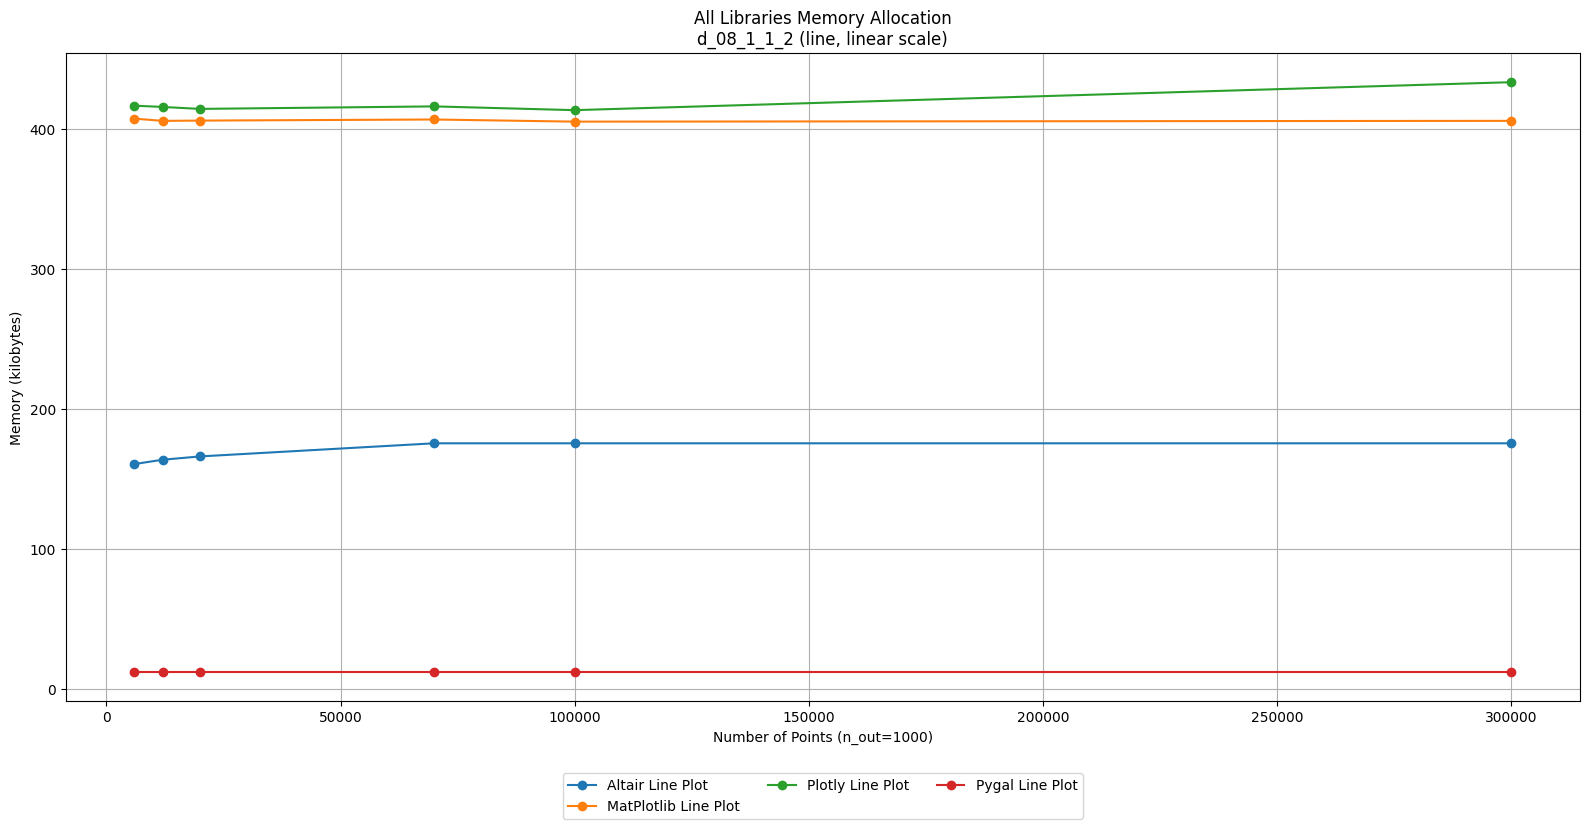
\includegraphics[width=1\textwidth]{anexo/exp/All Libraries Memory Allocation/plots/All Libraries Memory Allocation_d_08_1_1_2_linear_line.png}
        \caption[]{Gráfico de memoria asignada por las diferentes bibliotecas al crear un gráfico para el input \textbf{d\_08\_1\_1\_2}.}
        \label{fig:all_libraries_memory_allocation_plot_line_1}
    \end{figure}
}

\DeclareRobustCommand{\AllLibrariesMemoryAllocationOnePlotBar}{
    %insertar imagen
    \begin{figure}[H]
        \centering
        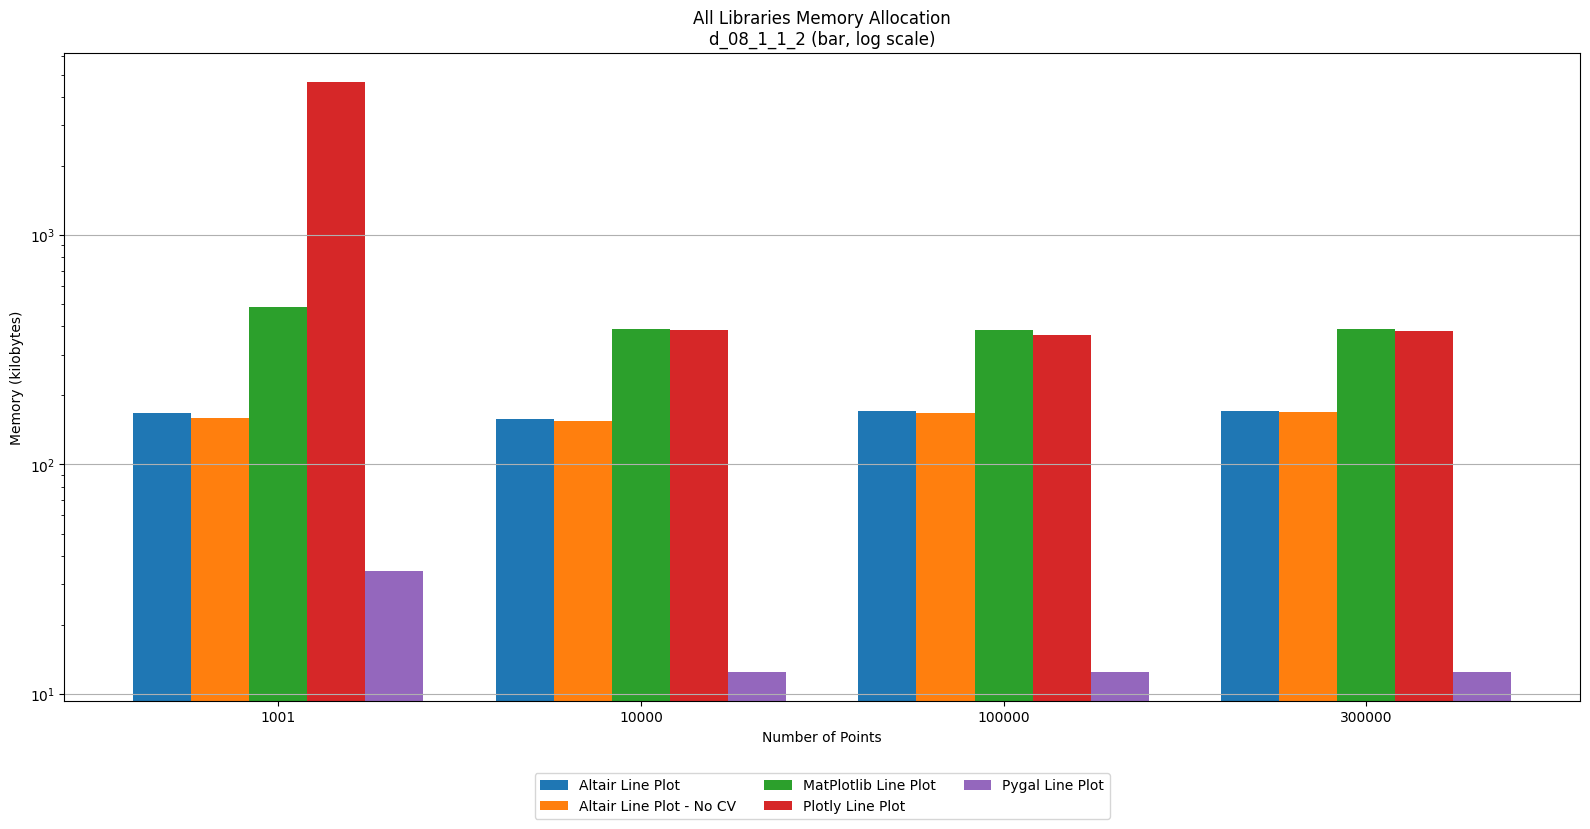
\includegraphics[width=1\textwidth]{anexo/exp/All Libraries Memory Allocation/bar_plots/All Libraries Memory Allocation_d_08_1_1_2_log_bar.png}
        \caption[]{Gráfico de memoria asignada por las diferentes bibliotecas al crear un gráfico para el input \textbf{d\_08\_1\_1\_2}.}
        \label{fig:all_libraries_memory_allocation_plot_bar_1}
    \end{figure}
}

\DeclareRobustCommand{\AllLibrariesMemoryAllocationTwoPlotLine}{
    %insertar imagen
    \begin{figure}[H]
        \centering
        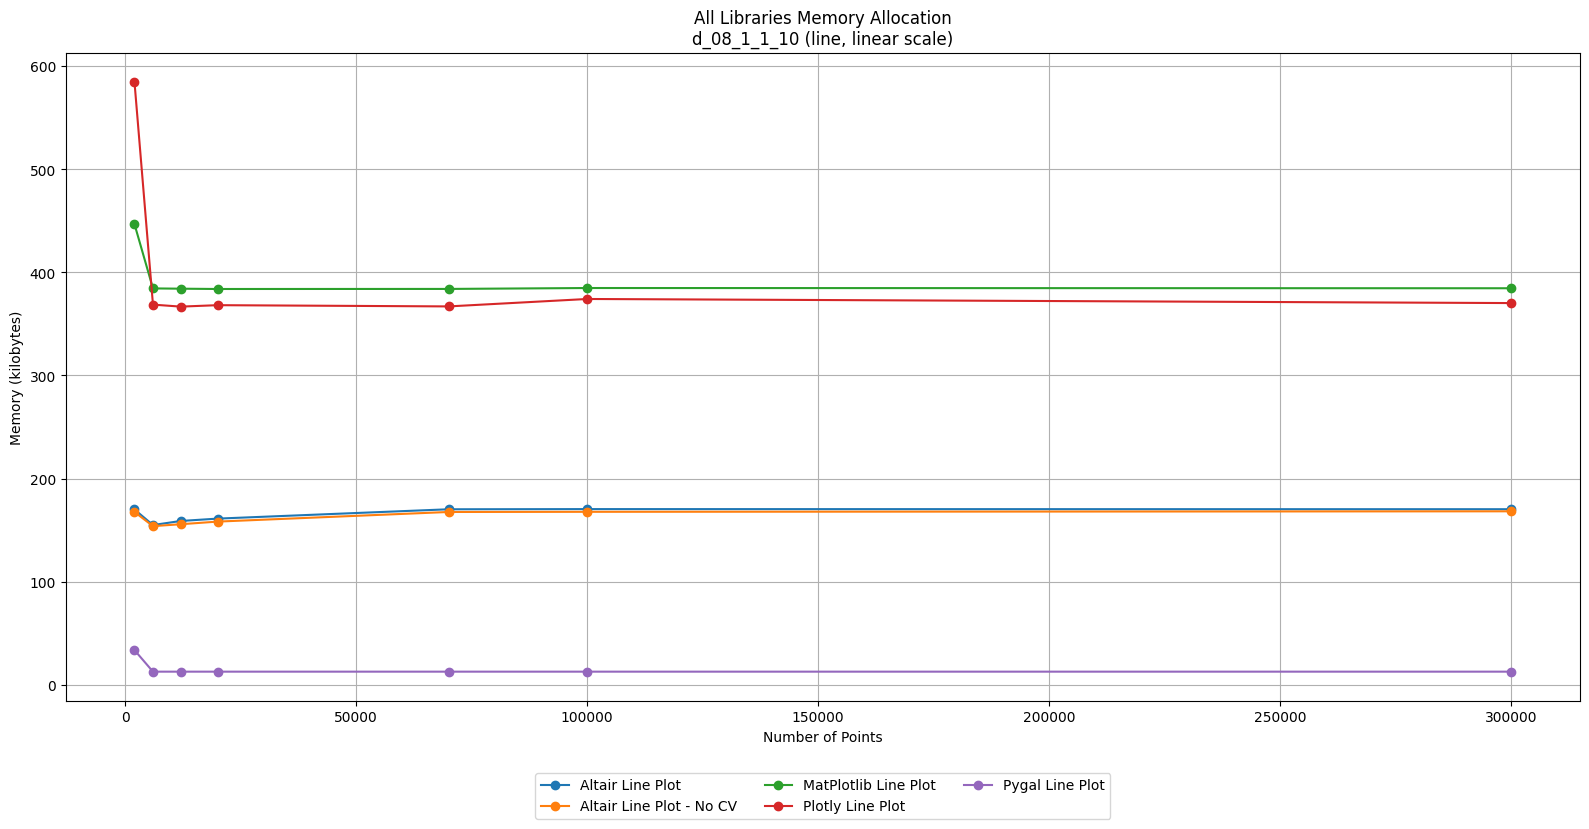
\includegraphics[width=1\textwidth]{anexo/exp/All Libraries Memory Allocation/plots/All Libraries Memory Allocation_d_08_1_1_10_linear_line.png}
        \caption[]{Gráfico de memoria asignada por las diferentes bibliotecas al crear un gráfico para el input \textbf{d\_08\_1\_1\_10}.}
        \label{fig:all_libraries_memory_allocation_plot_line_2}
    \end{figure}
}

\DeclareRobustCommand{\AllLibrariesMemoryAllocationTwoPlotBar}{
    %insertar imagen
    \begin{figure}[H]
        \centering
        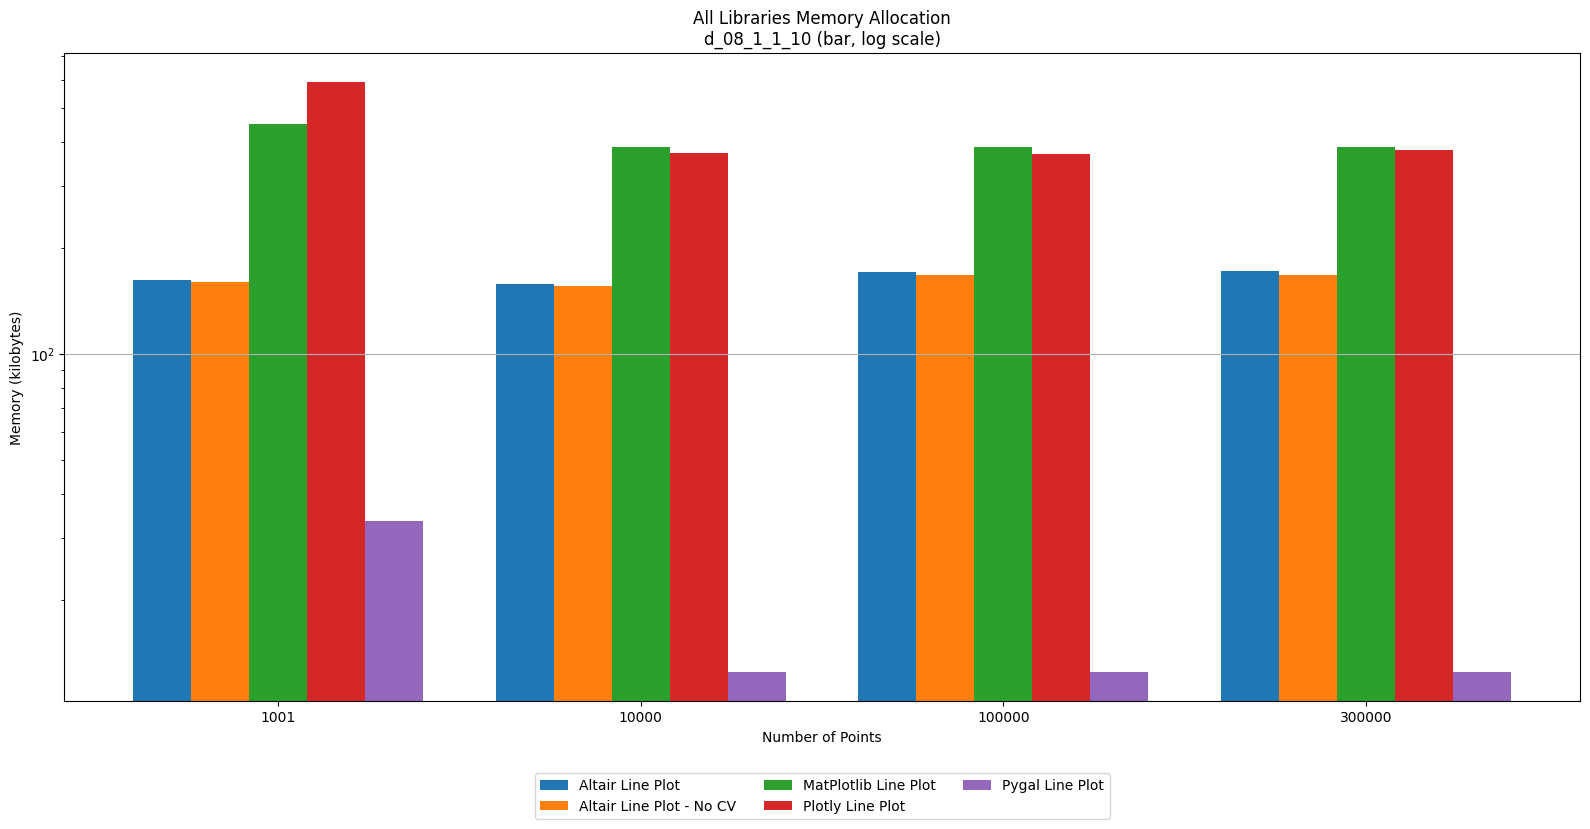
\includegraphics[width=1\textwidth]{anexo/exp/All Libraries Memory Allocation/bar_plots/All Libraries Memory Allocation_d_08_1_1_10_log_bar.png}
        \caption[]{Gráfico de memoria asignada por las diferentes bibliotecas al crear un gráfico para el input \textbf{d\_08\_1\_1\_10}.}
        \label{fig:all_libraries_memory_allocation_plot_bar_2}
    \end{figure}
}

\DeclareRobustCommand{\AllLibrariesMemoryAllocationThreePlotLine}{
    %insertar imagen
    \begin{figure}[H]
        \centering
        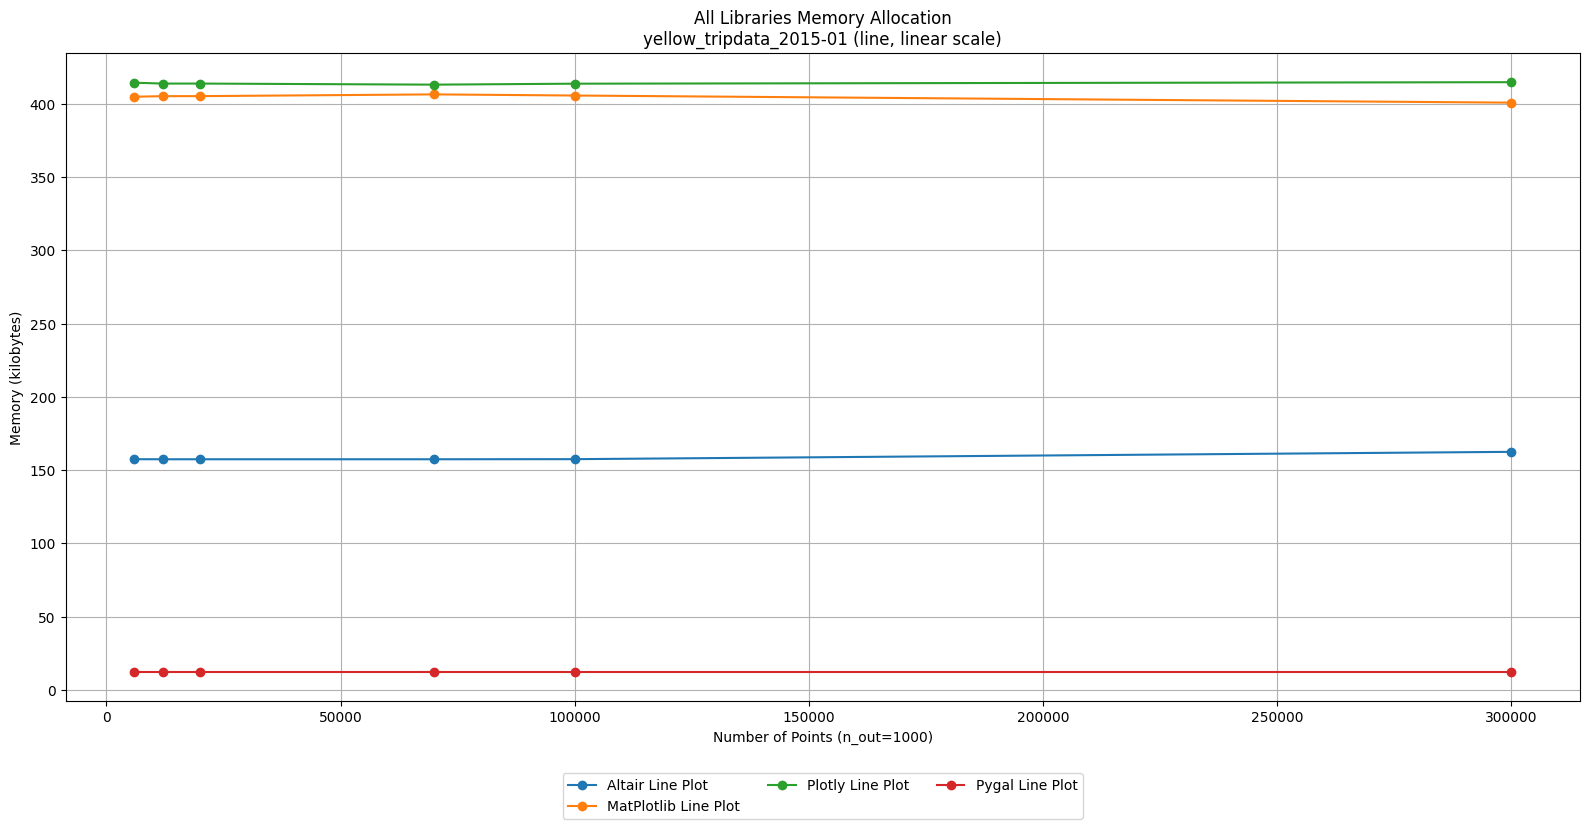
\includegraphics[width=1\textwidth]{anexo/exp/All Libraries Memory Allocation/plots/All Libraries Memory Allocation_yellow_tripdata_2015-01_linear_line.png}
        \caption[]{Gráfico de memoria asignada por las diferentes bibliotecas al crear un gráfico para el input \textbf{yellow\_tripdata\_2015\_01}.}
        \label{fig:all_libraries_memory_allocation_plot_line_3}
    \end{figure}
}

\DeclareRobustCommand{\AllLibrariesMemoryAllocationThreePlotBar}{
    %insertar imagen
    \begin{figure}[H]
        \centering
        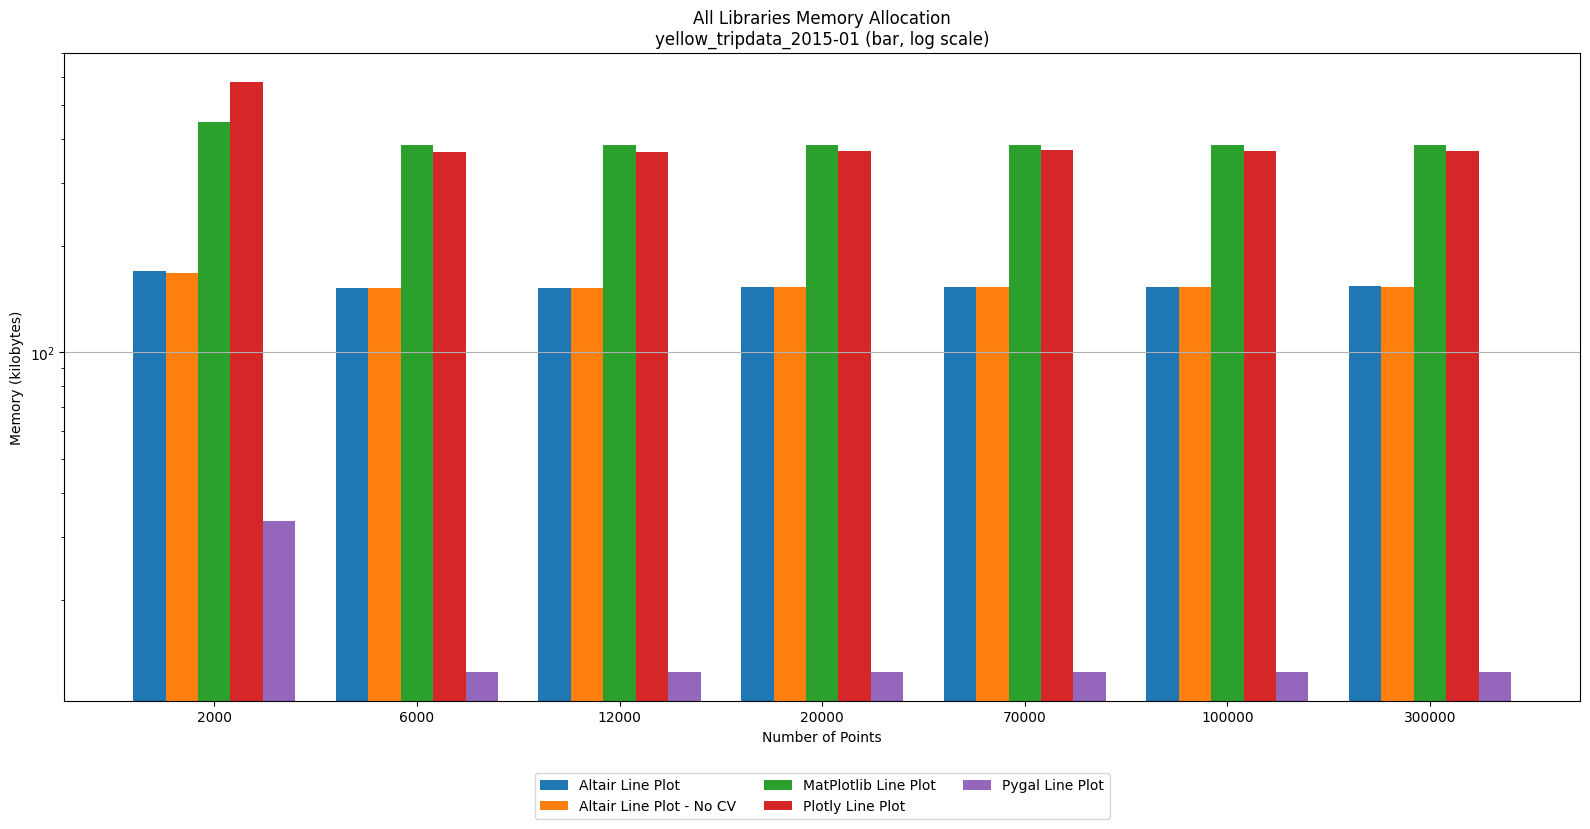
\includegraphics[width=1\textwidth]{anexo/exp/All Libraries Memory Allocation/bar_plots/All Libraries Memory Allocation_yellow_tripdata_2015-01_log_bar.png}
        \caption[]{Gráfico de memoria asignada por las diferentes bibliotecas al crear un gráfico para el input \textbf{yellow\_tripdata\_2015\_01}.}
        \label{fig:all_libraries_memory_allocation_plot_bar_3}
    \end{figure}
}




% All Libraries Time Comparison
\DeclareRobustCommand{\AllLibrariesTimeComparisonOnePlotLine}{
    %insertar imagen
    \begin{figure}[H]
        \centering
        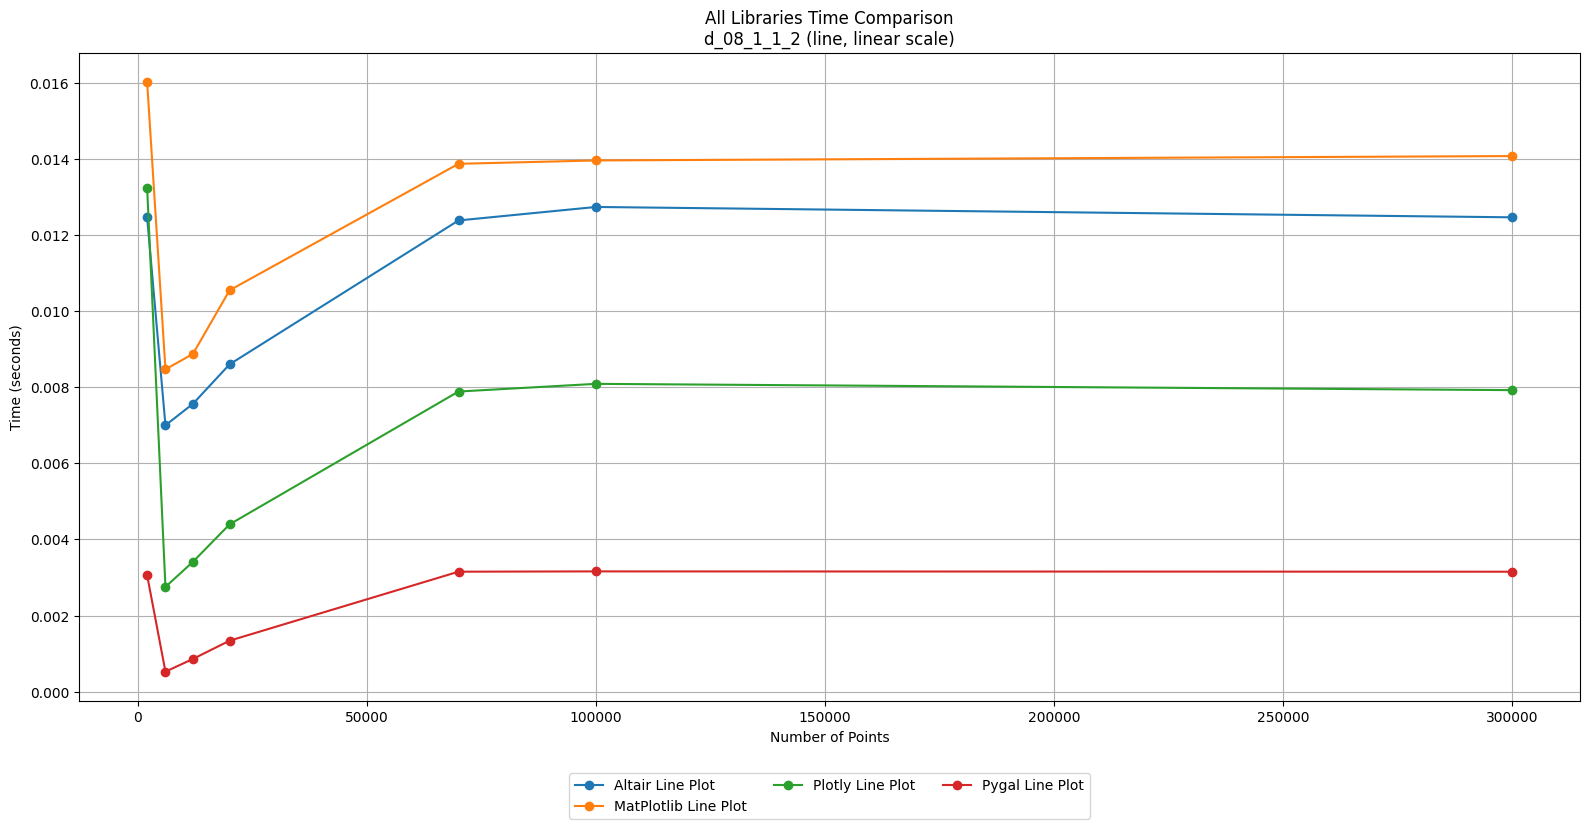
\includegraphics[width=1\textwidth]{anexo/exp/All Libraries Time Comparison/plots/All Libraries Time Comparison_d_08_1_1_2_linear_line.png}
        \caption[]{Gráfico de tiempo de ejecución de las diferentes bibliotecas al crear un gráfico para el input \textbf{d\_08\_1\_1\_2}.}
        \label{fig:all_libraries_time_comparison_plot_line_1}
    \end{figure}
}

\DeclareRobustCommand{\AllLibrariesTimeComparisonOnePlotBar}{
    %insertar imagen
    \begin{figure}[H]
        \centering
        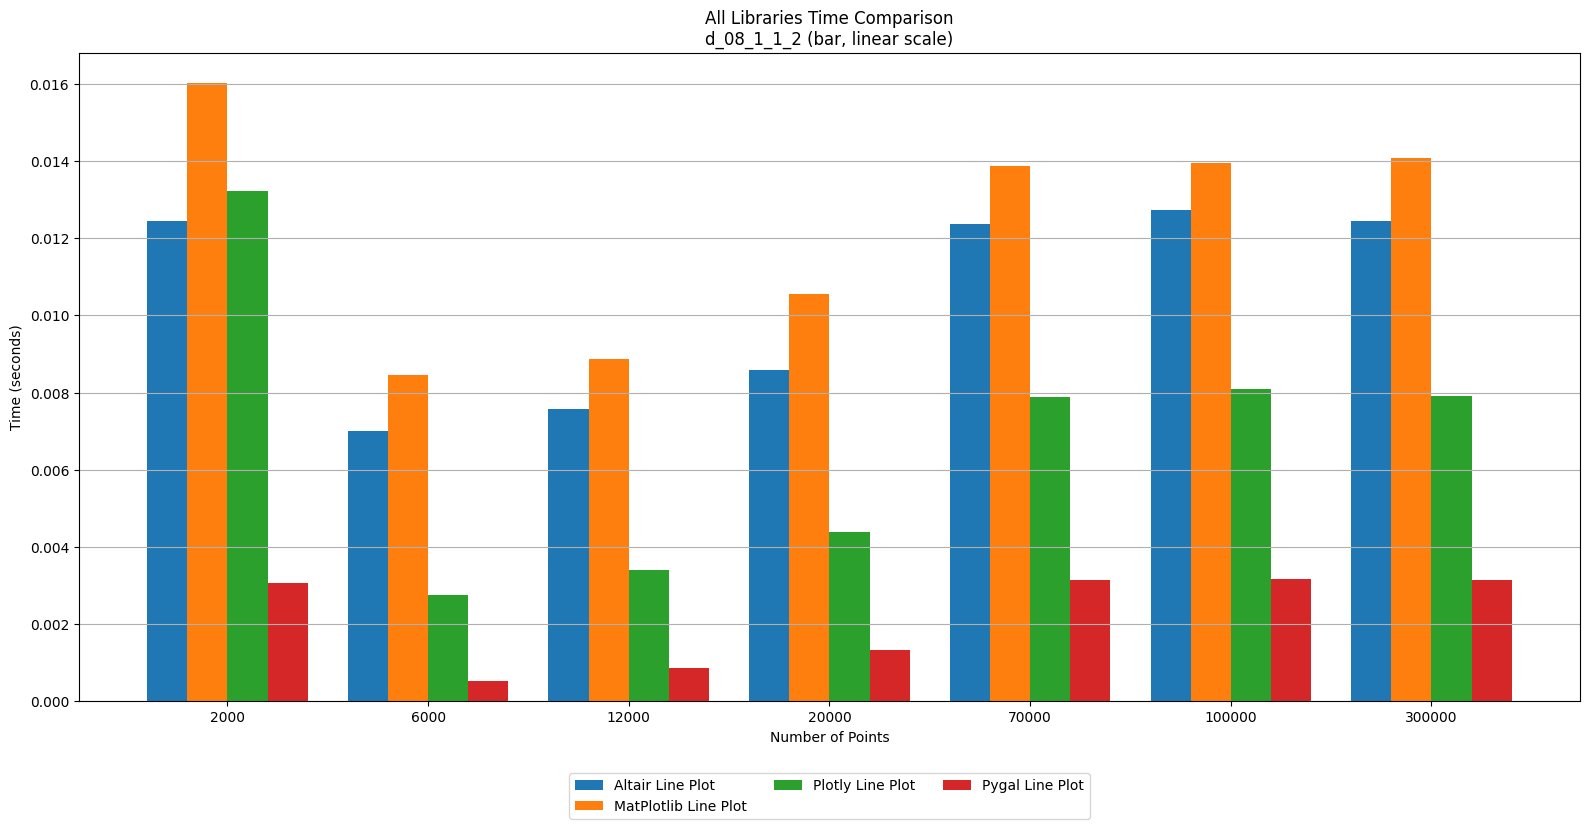
\includegraphics[width=1\textwidth]{anexo/exp/All Libraries Time Comparison/bar_plots/All Libraries Time Comparison_d_08_1_1_2_linear_bar.png}
        \caption[]{Gráfico de tiempo de ejecución de las diferentes bibliotecas al crear un gráfico para el input \textbf{d\_08\_1\_1\_2}.}
        \label{fig:all_libraries_time_comparison_plot_bar_1}
    \end{figure}
}

\DeclareRobustCommand{\AllLibrariesTimeComparisonTwoPlotLine}{
    %insertar imagen
    \begin{figure}[H]
        \centering
        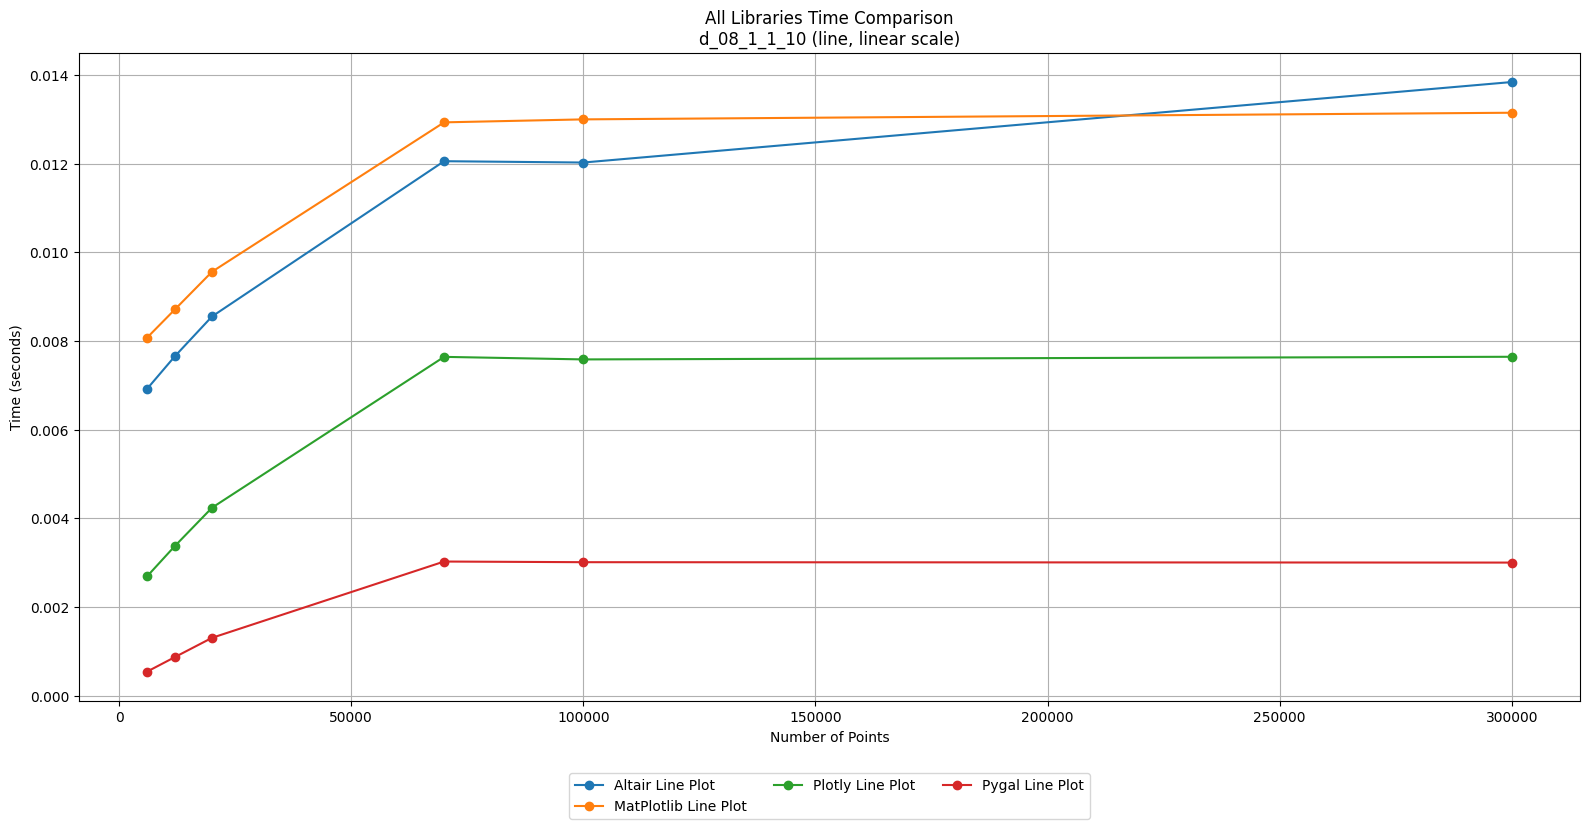
\includegraphics[width=1\textwidth]{anexo/exp/All Libraries Time Comparison/plots/All Libraries Time Comparison_d_08_1_1_10_linear_line.png}
        \caption[]{Gráfico de tiempo de ejecución de las diferentes bibliotecas al crear un gráfico para el input \textbf{d\_08\_1\_1\_10}.}
        \label{fig:all_libraries_time_comparison_plot_line_2}
    \end{figure}
}

\DeclareRobustCommand{\AllLibrariesTimeComparisonTwoPlotBar}{
    %insertar imagen
    \begin{figure}[H]
        \centering
        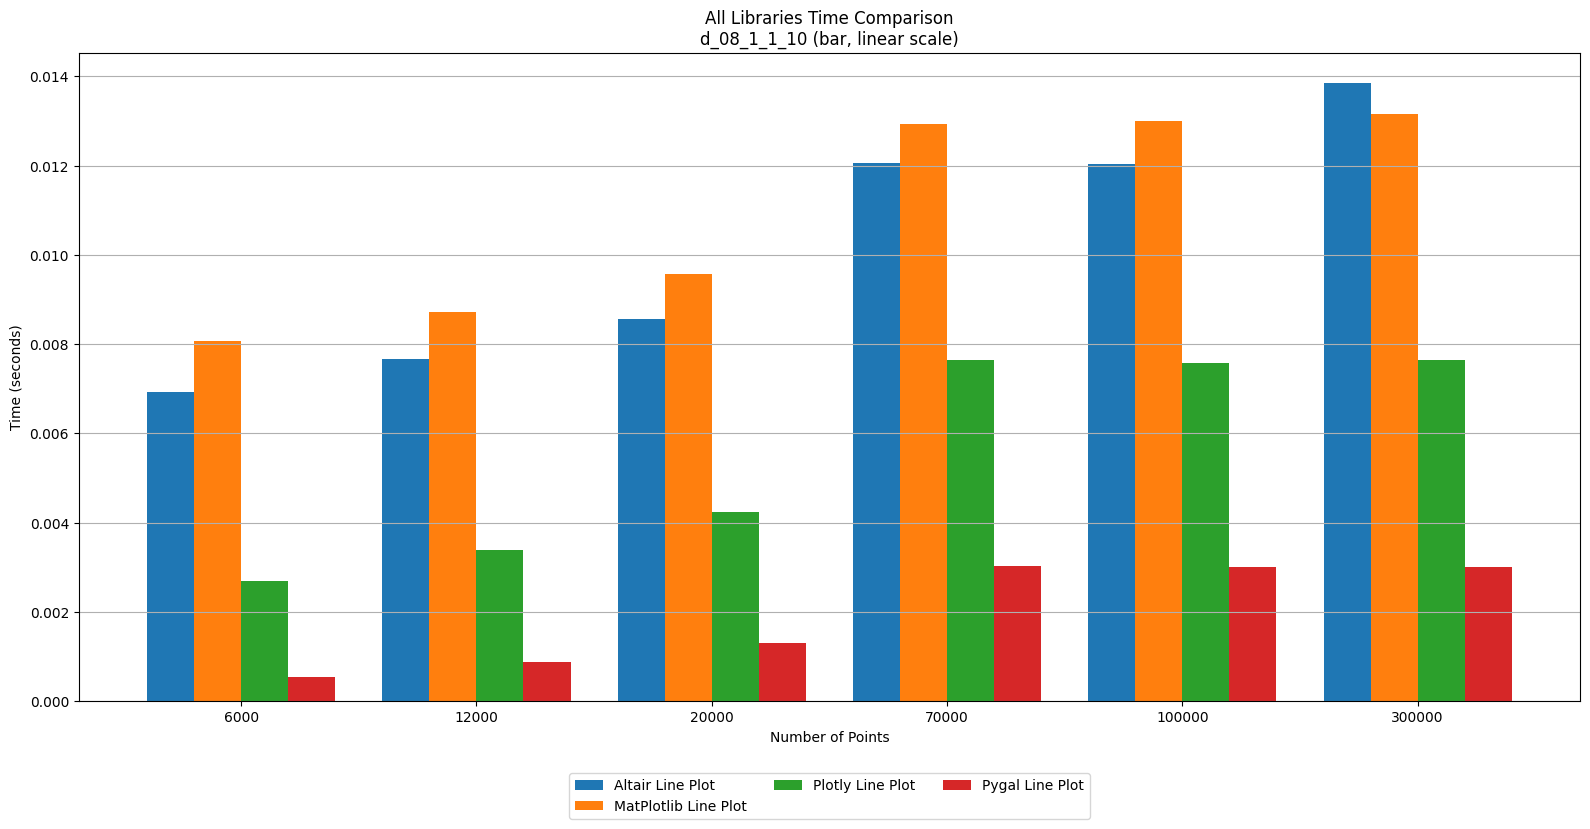
\includegraphics[width=1\textwidth]{anexo/exp/All Libraries Time Comparison/bar_plots/All Libraries Time Comparison_d_08_1_1_10_linear_bar.png}
        \caption[]{Gráfico de tiempo de ejecución de las diferentes bibliotecas al crear un gráfico para el input \textbf{d\_08\_1\_1\_10}.}
        \label{fig:all_libraries_time_comparison_plot_bar_2}
    \end{figure}
}

\DeclareRobustCommand{\AllLibrariesTimeComparisonThreePlotLine}{
    %insertar imagen
    \begin{figure}[H]
        \centering
        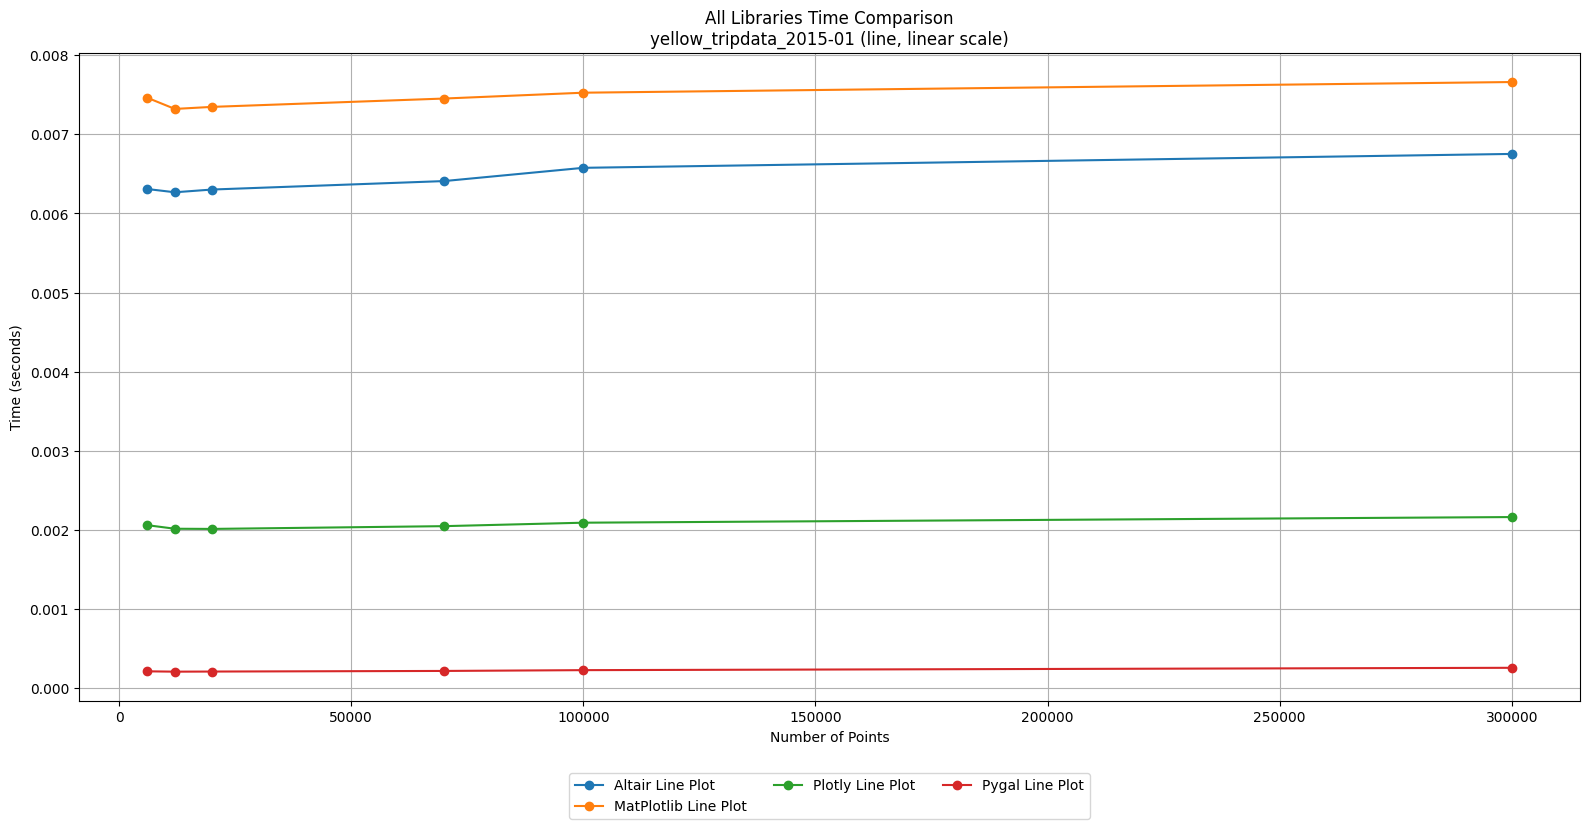
\includegraphics[width=1\textwidth]{anexo/exp/All Libraries Time Comparison/plots/All Libraries Time Comparison_yellow_tripdata_2015-01_linear_line.png}
        \caption[]{Gráfico de tiempo de ejecución de las diferentes bibliotecas al crear un gráfico para el input \textbf{yellow\_tripdata\_2015\_01}.}
        \label{fig:all_libraries_time_comparison_plot_line_3}
    \end{figure}
}

\DeclareRobustCommand{\AllLibrariesTimeComparisonThreePlotBar}{
    %insertar imagen
    \begin{figure}[H]
        \centering
        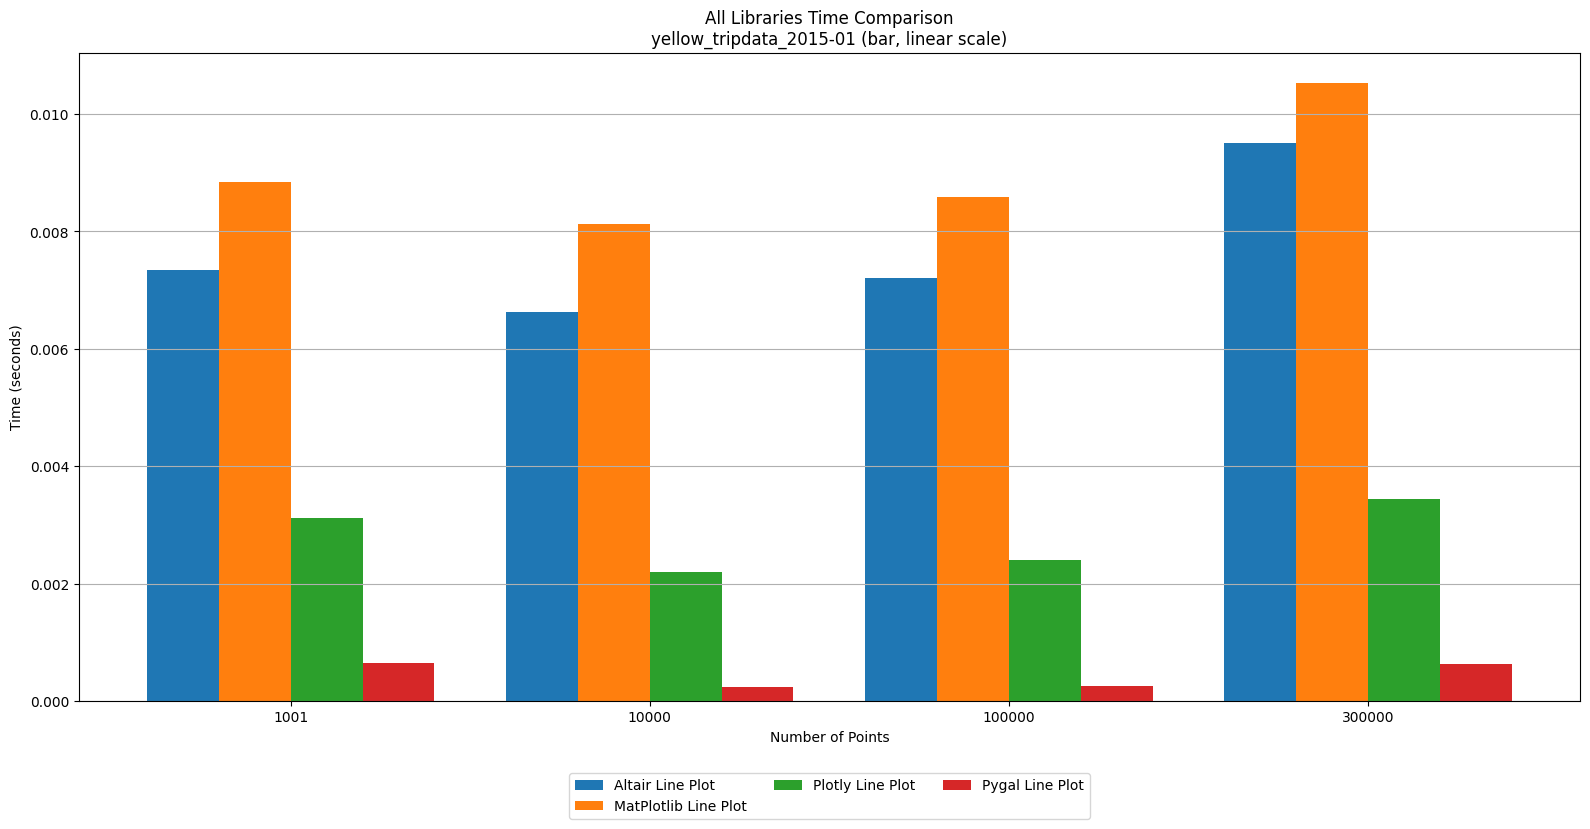
\includegraphics[width=1\textwidth]{anexo/exp/All Libraries Time Comparison/bar_plots/All Libraries Time Comparison_yellow_tripdata_2015-01_linear_bar.png}
        \caption[]{Gráfico de tiempo de ejecución de las diferentes bibliotecas al crear un gráfico para el input \textbf{yellow\_tripdata\_2015\_01}.}
        \label{fig:all_libraries_time_comparison_plot_bar_3}
    \end{figure}
}

Building Time Comparison
\DeclareRobustCommand{\BuildingTimeComparisonOnePlotLine}{
    %insertar imagen
    \begin{figure}[H]
        \centering
        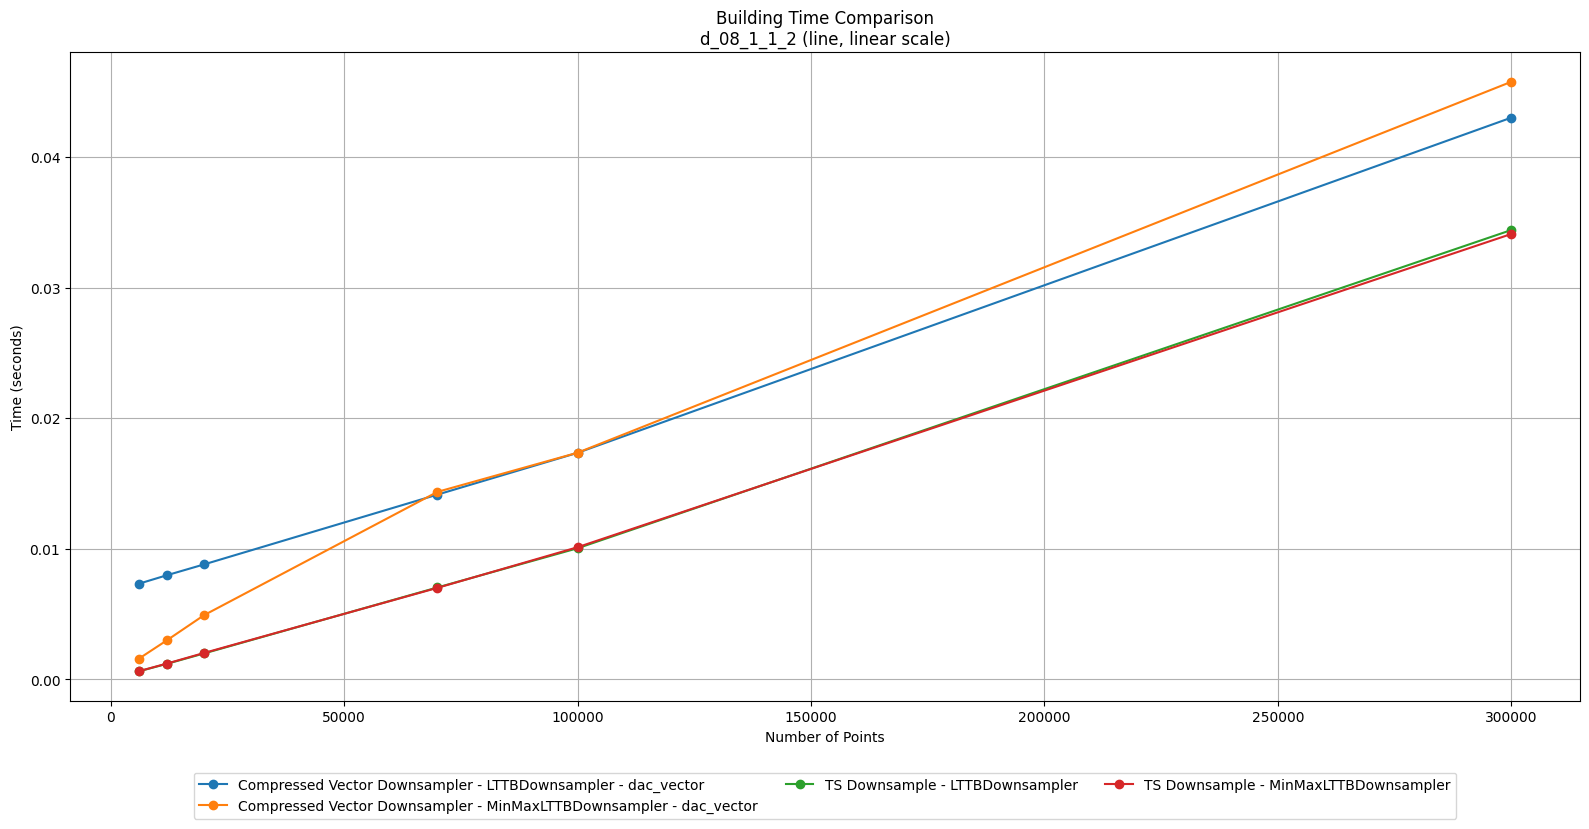
\includegraphics[width=1\textwidth]{anexo/exp/Building Time Comparison/plots/Building Time Comparison_d_08_1_1_2_linear_line.png}
        \caption[]{Gráfico de tiempo de construcción de las diferentes bibliotecas para el input \textbf{d\_08\_1\_1\_2}.}
        \label{fig:building_time_comparison_plot_line_1}
    \end{figure}
}

\DeclareRobustCommand{\BuildingTimeComparisonOnePlotBar}{
    %insertar imagen
    \begin{figure}[H]
        \centering
        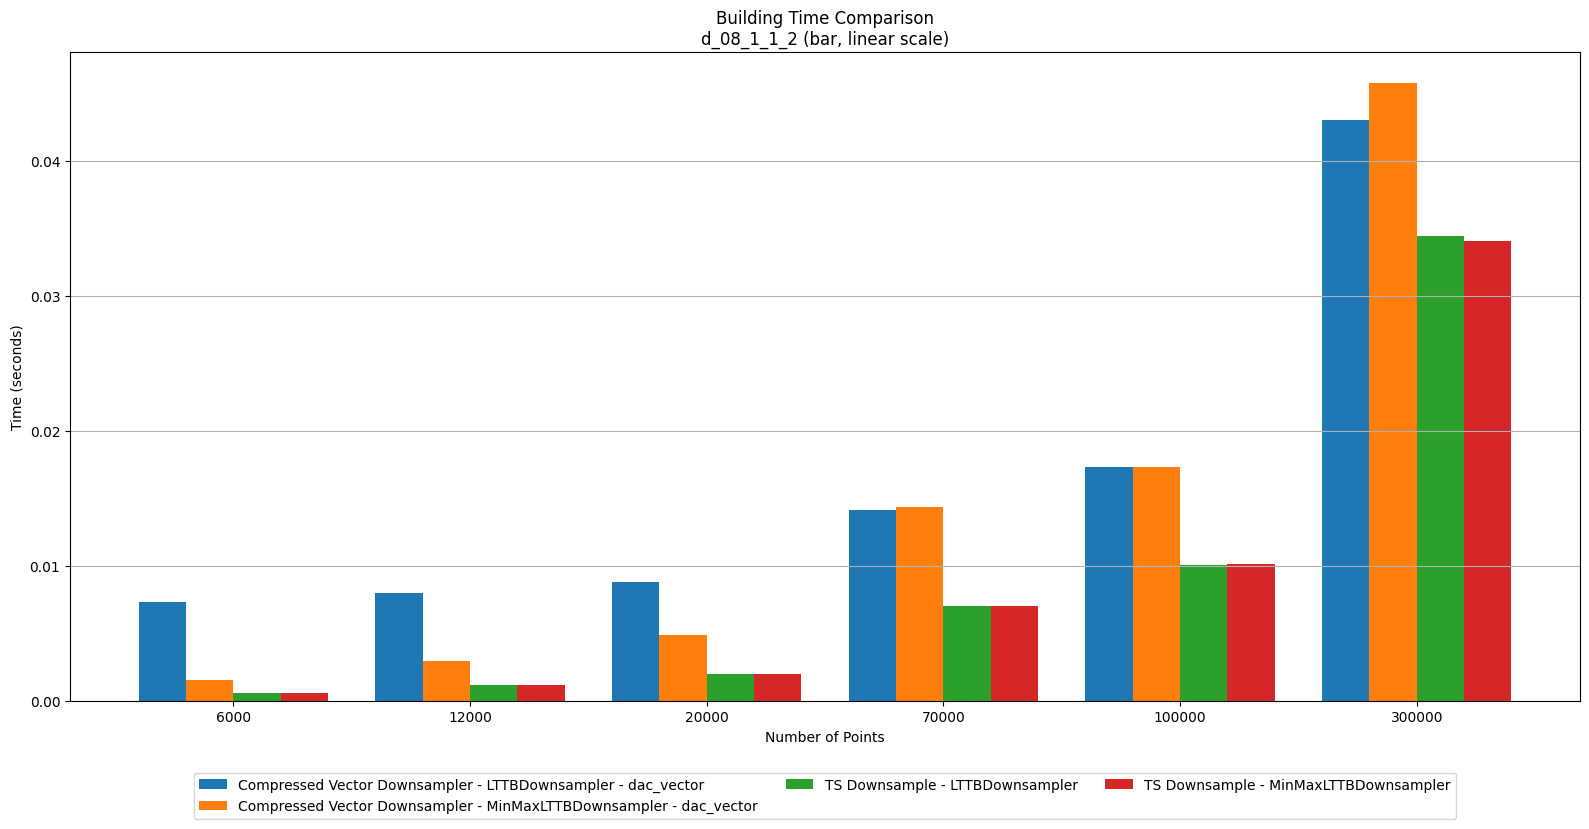
\includegraphics[width=1\textwidth]{anexo/exp/Building Time Comparison/bar_plots/Building Time Comparison_d_08_1_1_2_linear_bar.png}
        \caption[]{Gráfico de tiempo de construcción de las diferentes bibliotecas para el input \textbf{d\_08\_1\_1\_2}.}
        \label{fig:building_time_comparison_plot_bar_1}
    \end{figure}
}

\DeclareRobustCommand{\BuildingTimeComparisonTwoPlotLine}{
    %insertar imagen
    \begin{figure}[H]
        \centering
        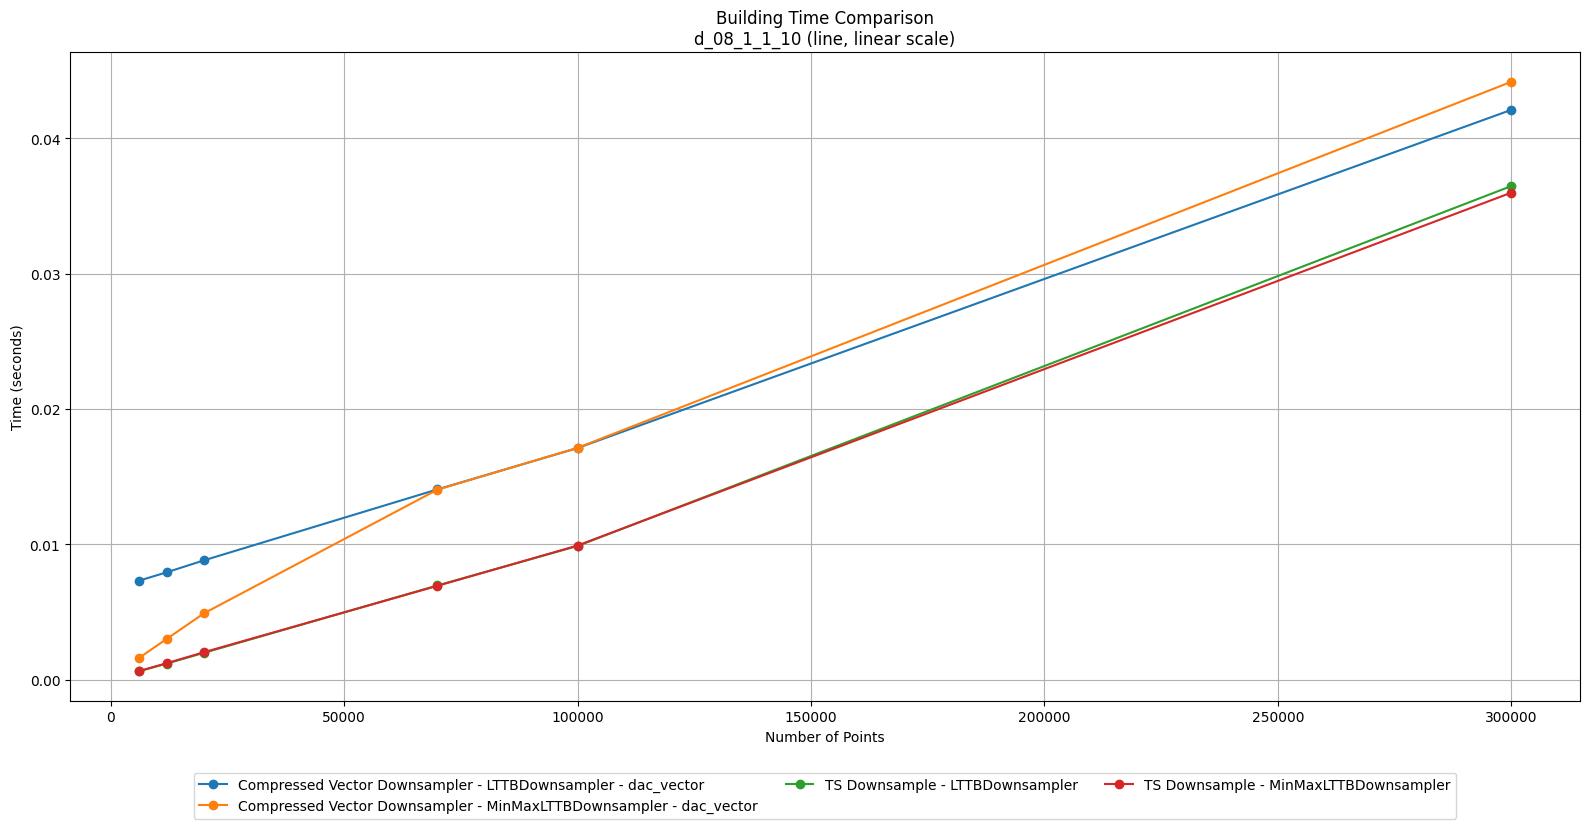
\includegraphics[width=1\textwidth]{anexo/exp/Building Time Comparison/plots/Building Time Comparison_d_08_1_1_10_linear_line.png}
        \caption[]{Gráfico de tiempo de construcción de las diferentes bibliotecas para el input \textbf{d\_08\_1\_1\_10}.}
        \label{fig:building_time_comparison_plot_line_2}
    \end{figure}
}

\DeclareRobustCommand{\BuildingTimeComparisonTwoPlotBar}{
    %insertar imagen
    \begin{figure}[H]
        \centering
        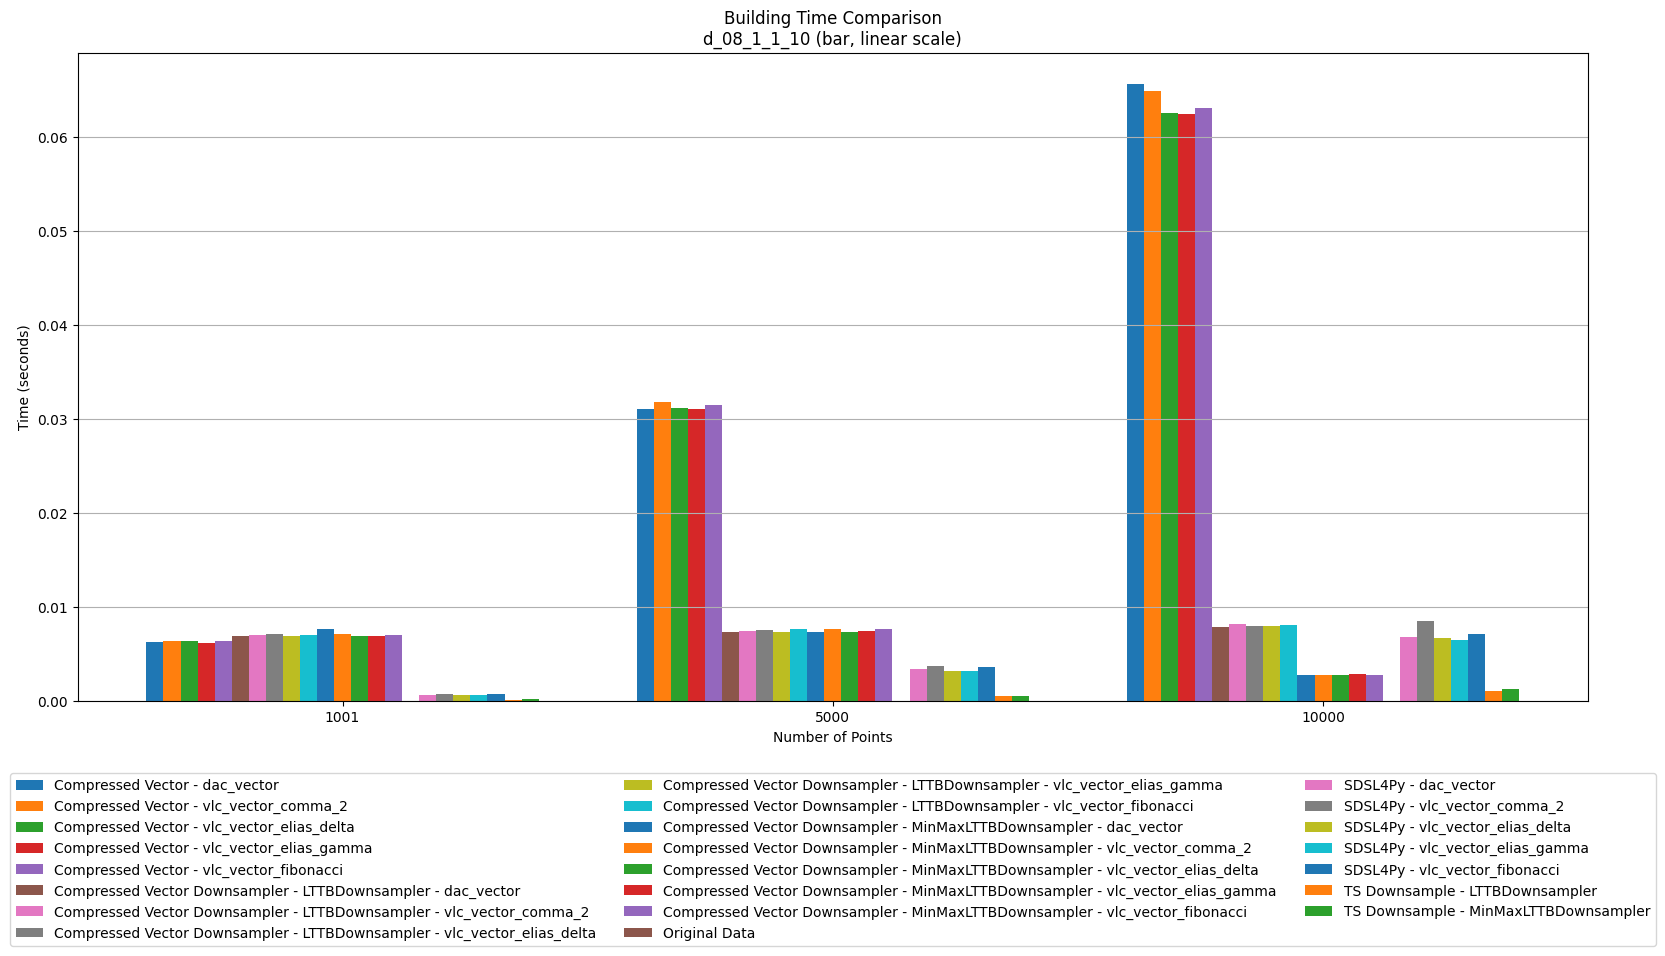
\includegraphics[width=1\textwidth]{anexo/exp/Building Time Comparison/bar_plots/Building Time Comparison_d_08_1_1_10_linear_bar.png}
        \caption[]{Gráfico de tiempo de construcción de las diferentes bibliotecas para el input \textbf{d\_08\_1\_1\_10}.}
        \label{fig:building_time_comparison_plot_bar_2}
    \end{figure}
}

\DeclareRobustCommand{\BuildingTimeComparisonThreePlotLine}{
    %insertar imagen
    \begin{figure}[H]
        \centering
        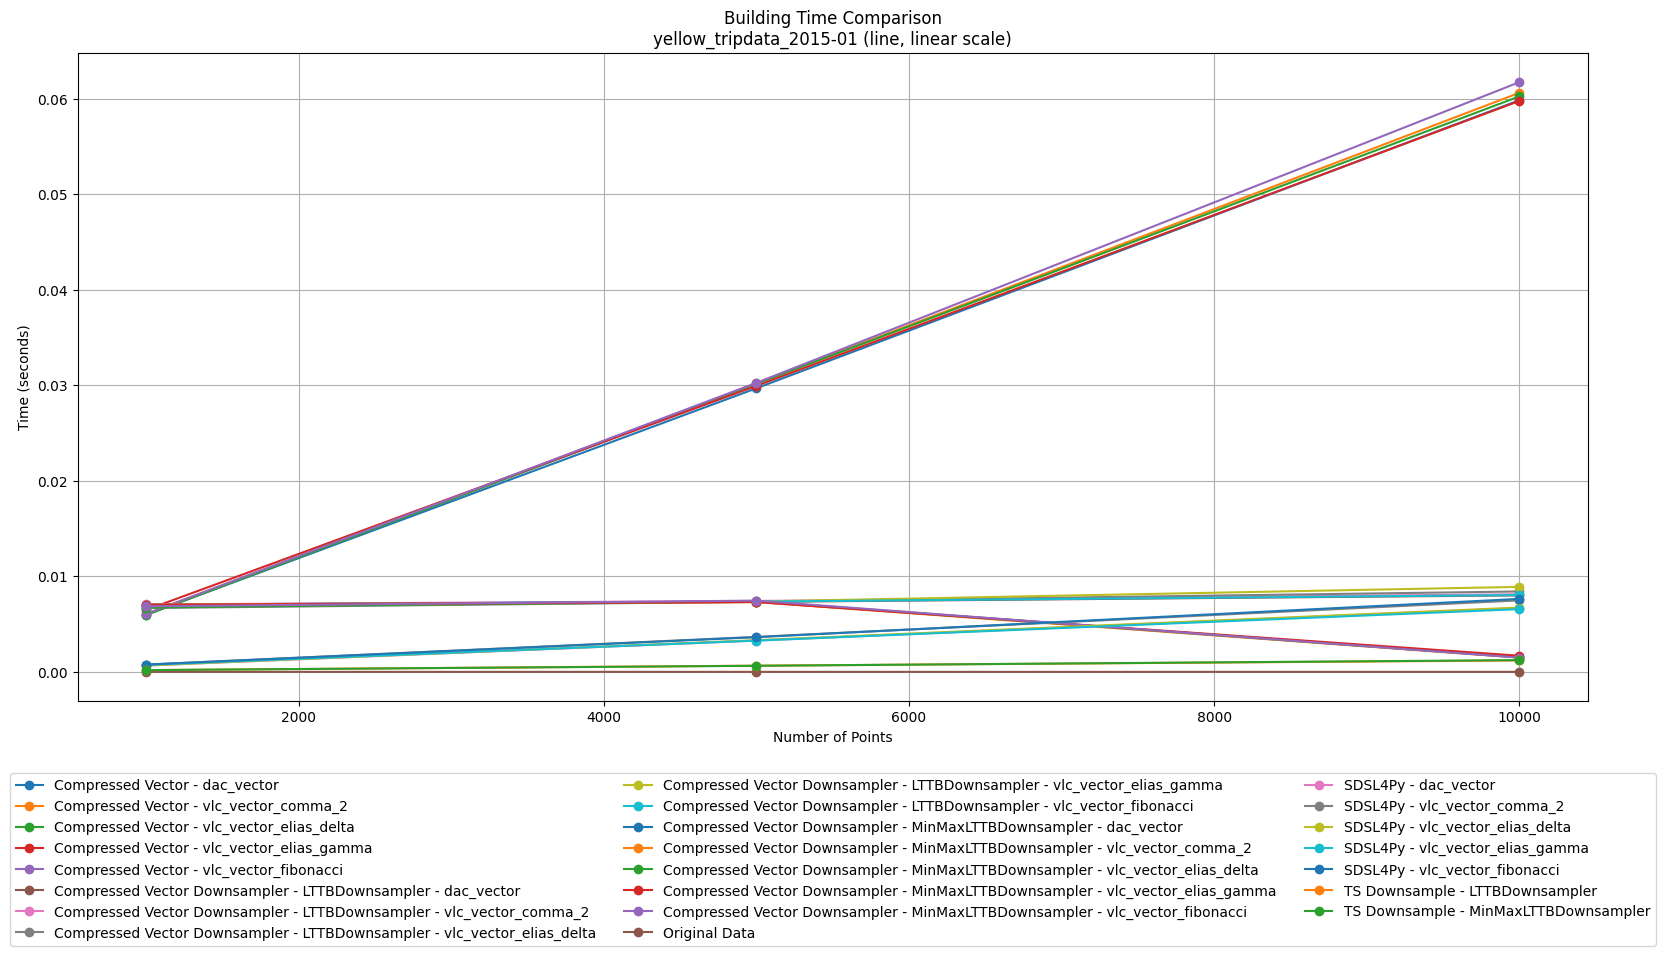
\includegraphics[width=1\textwidth]{anexo/exp/Building Time Comparison/plots/Building Time Comparison_yellow_tripdata_2015-01_linear_line.png}
        \caption[]{Gráfico de tiempo de construcción de las diferentes bibliotecas para el input \textbf{yellow\_tripdata\_2015\_01}.}
        \label{fig:building_time_comparison_plot_line_3}
    \end{figure}
}

\DeclareRobustCommand{\BuildingTimeComparisonThreePlotBar}{
    %insertar imagen
    \begin{figure}[H]
        \centering
        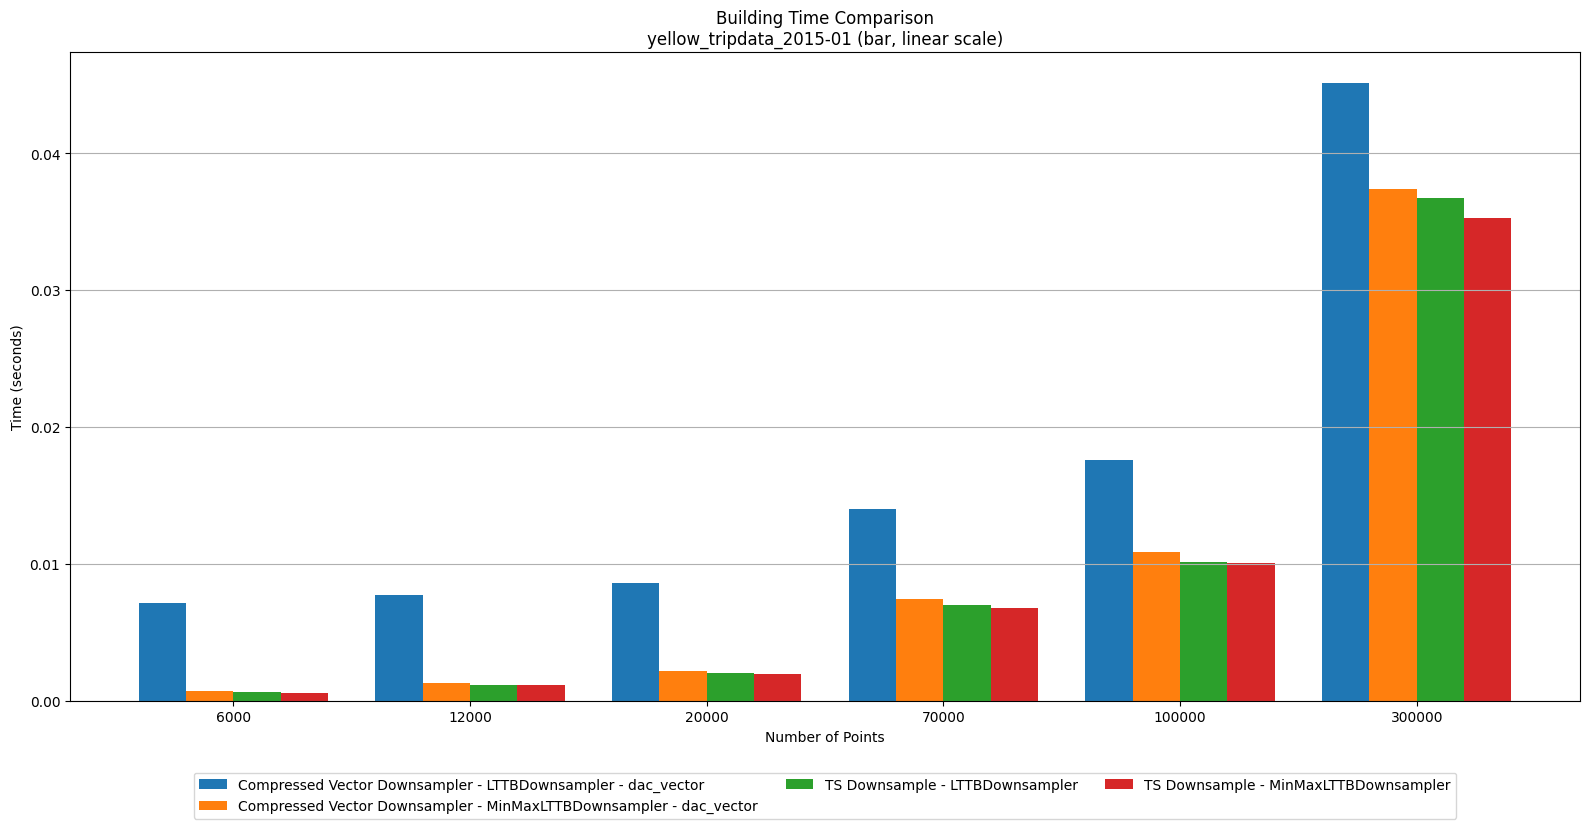
\includegraphics[width=1\textwidth]{anexo/exp/Building Time Comparison/bar_plots/Building Time Comparison_yellow_tripdata_2015-01_linear_bar.png}
        \caption[]{Gráfico de tiempo de construcción de las diferentes bibliotecas para el input \textbf{yellow\_tripdata\_2015\_01}.}
        \label{fig:building_time_comparison_plot_bar_3}
    \end{figure}
}




% Comparison of Space Used
\DeclareRobustCommand{\ComparisonOfSpaceUsedOnePlotLine}{
    %insertar imagen
    \begin{figure}[H]
        \centering
        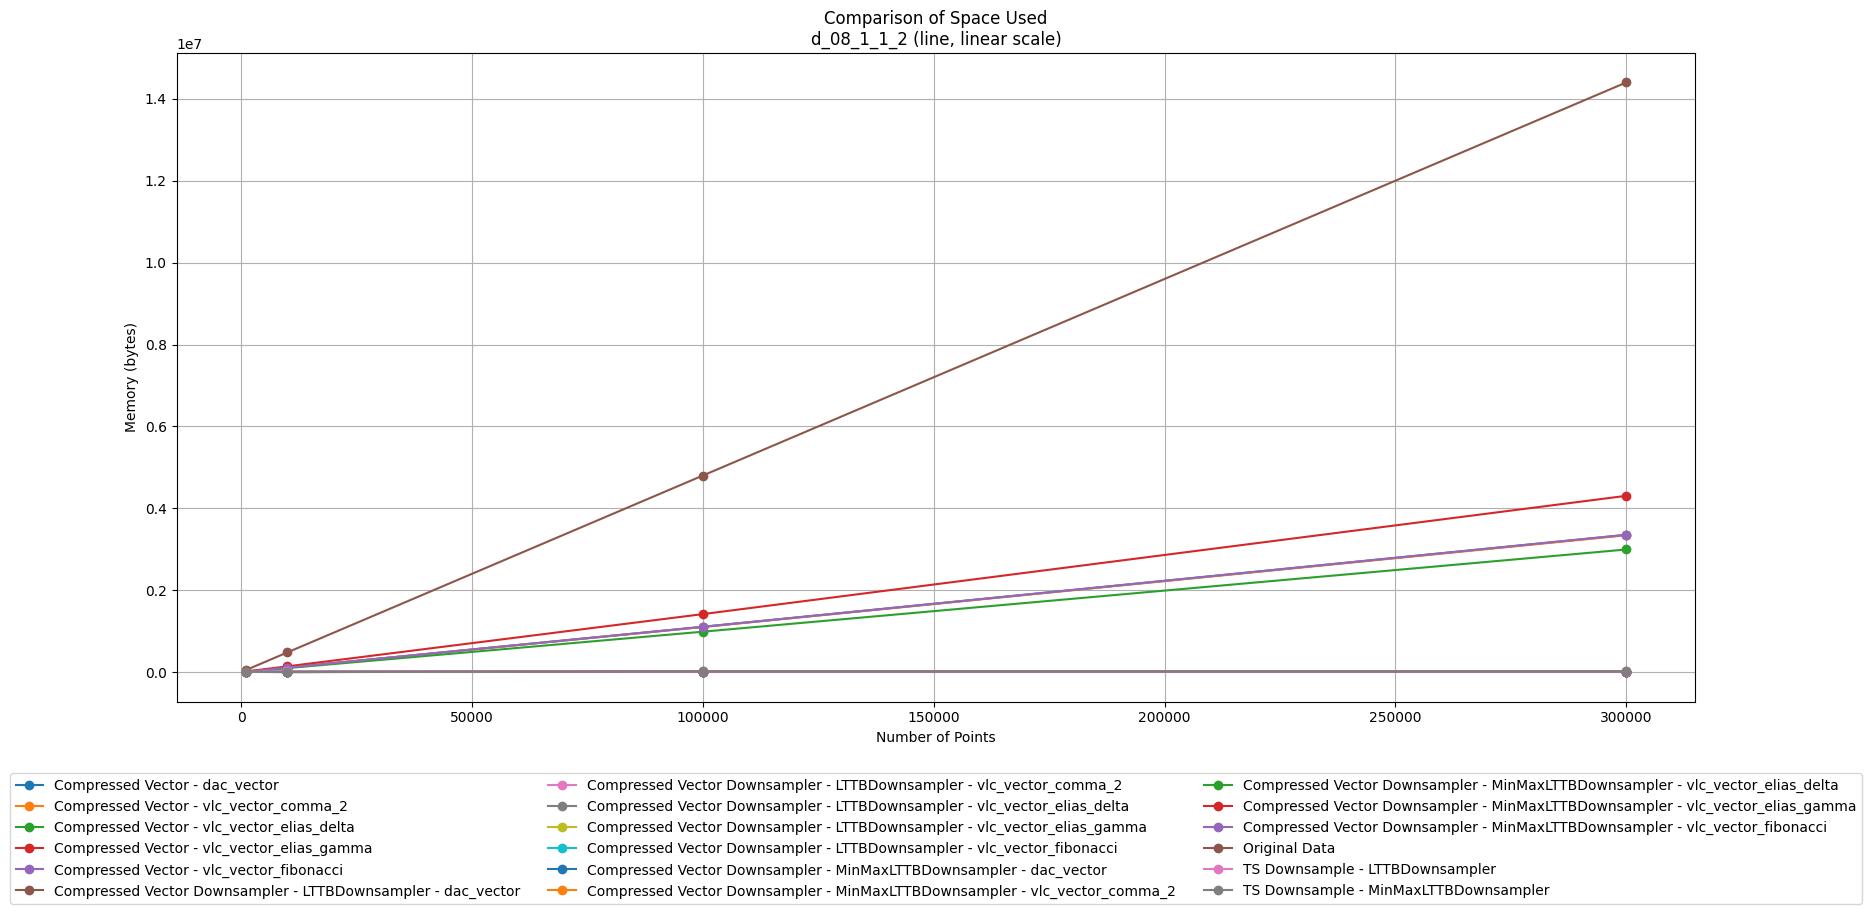
\includegraphics[width=1\textwidth]{anexo/exp/Comparison of Space Used/plots/Comparison of Space Used_d_08_1_1_2_linear_line.png}
        \caption[]{Gráfico de espacio usado por las diferentes bibliotecas para el input \textbf{d\_08\_1\_1\_2}.}
        \label{fig:comparison_of_space_used_plot_line_1}
    \end{figure}
}

\DeclareRobustCommand{\ComparisonOfSpaceUsedOnePlotBar}{
    %insertar imagen
    \begin{figure}[H]
        \centering
        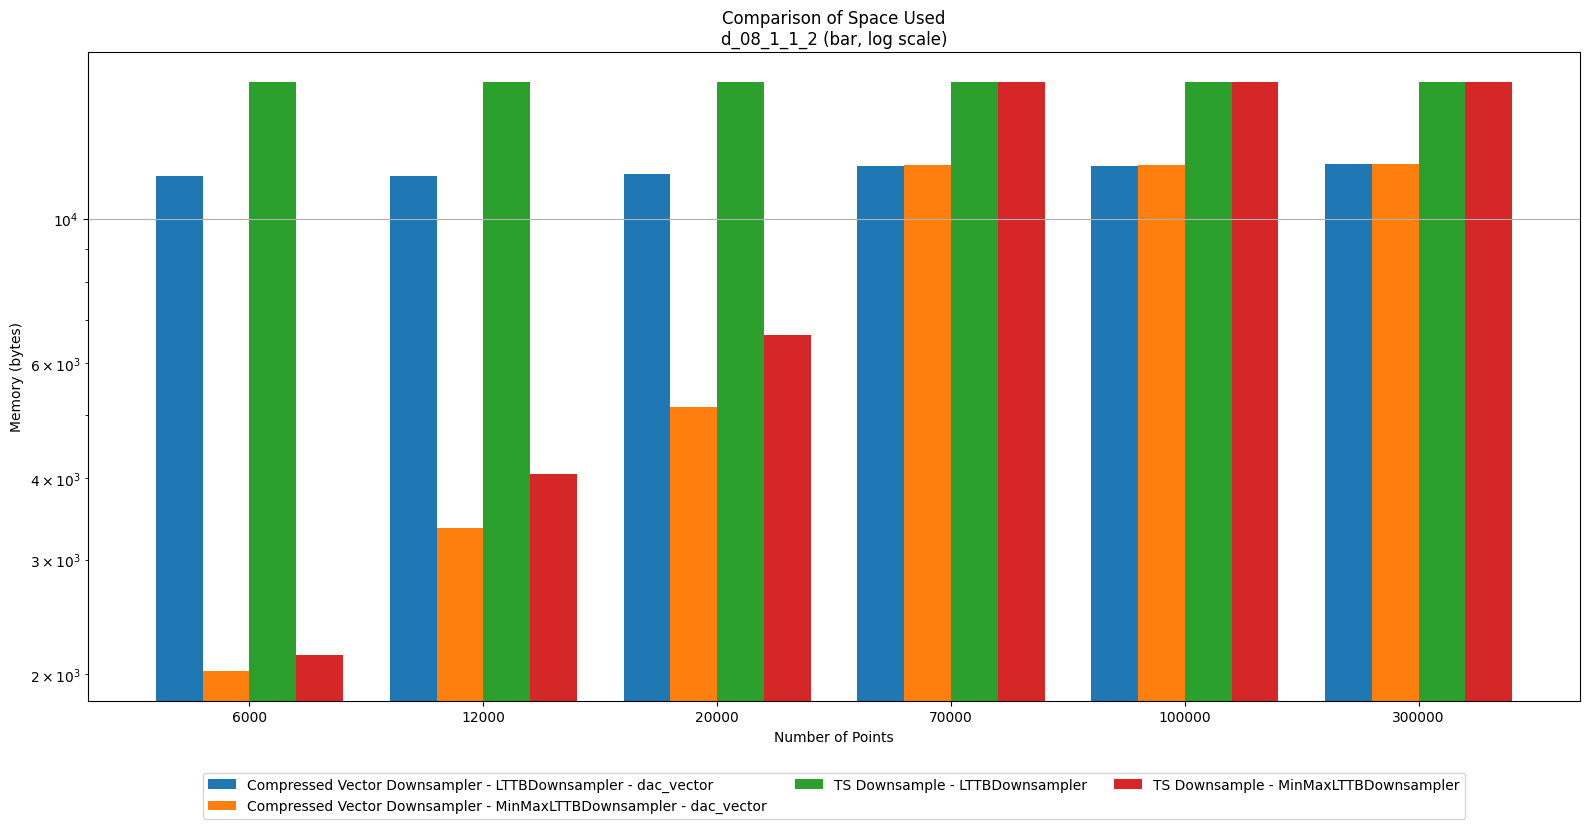
\includegraphics[width=1\textwidth]{anexo/exp/Comparison of Space Used/bar_plots/Comparison of Space Used_d_08_1_1_2_log_bar.png}
        \caption[]{Gráfico de espacio usado por las diferentes bibliotecas para el input \textbf{d\_08\_1\_1\_2}.}
        \label{fig:comparison_of_space_used_plot_bar_1}
    \end{figure}
}

\DeclareRobustCommand{\ComparisonOfSpaceUsedTwoPlotLine}{
    %insertar imagen
    \begin{figure}[H]
        \centering
        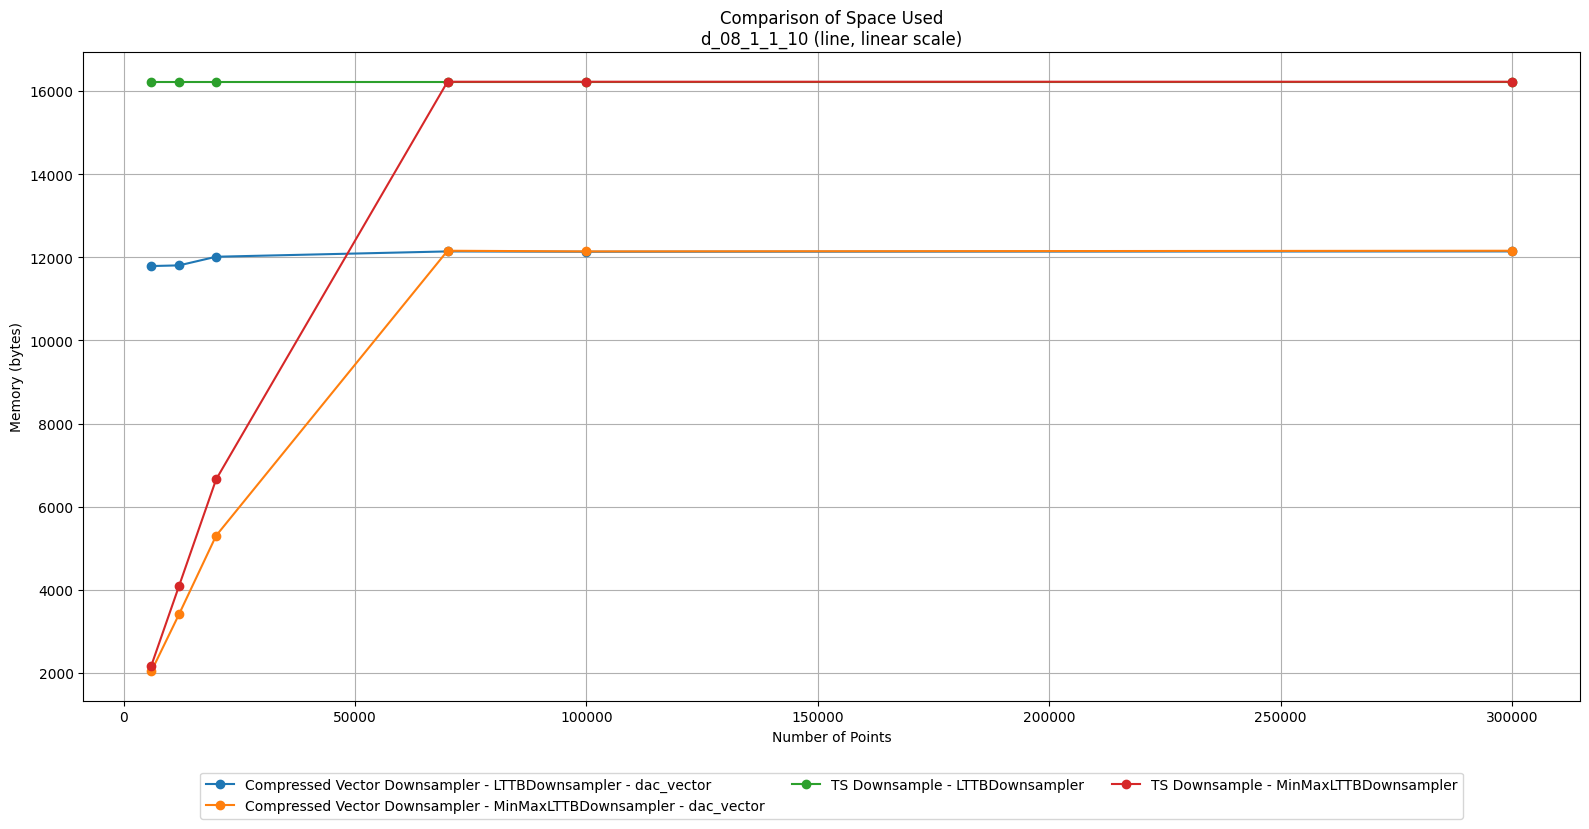
\includegraphics[width=1\textwidth]{anexo/exp/Comparison of Space Used/plots/Comparison of Space Used_d_08_1_1_10_linear_line.png}
        \caption[]{Gráfico de espacio usado por las diferentes bibliotecas para el input \textbf{d\_08\_1\_1\_10}.}
        \label{fig:comparison_of_space_used_plot_line_2}
    \end{figure}
}

\DeclareRobustCommand{\ComparisonOfSpaceUsedTwoPlotBar}{
    %insertar imagen
    \begin{figure}[H]
        \centering
        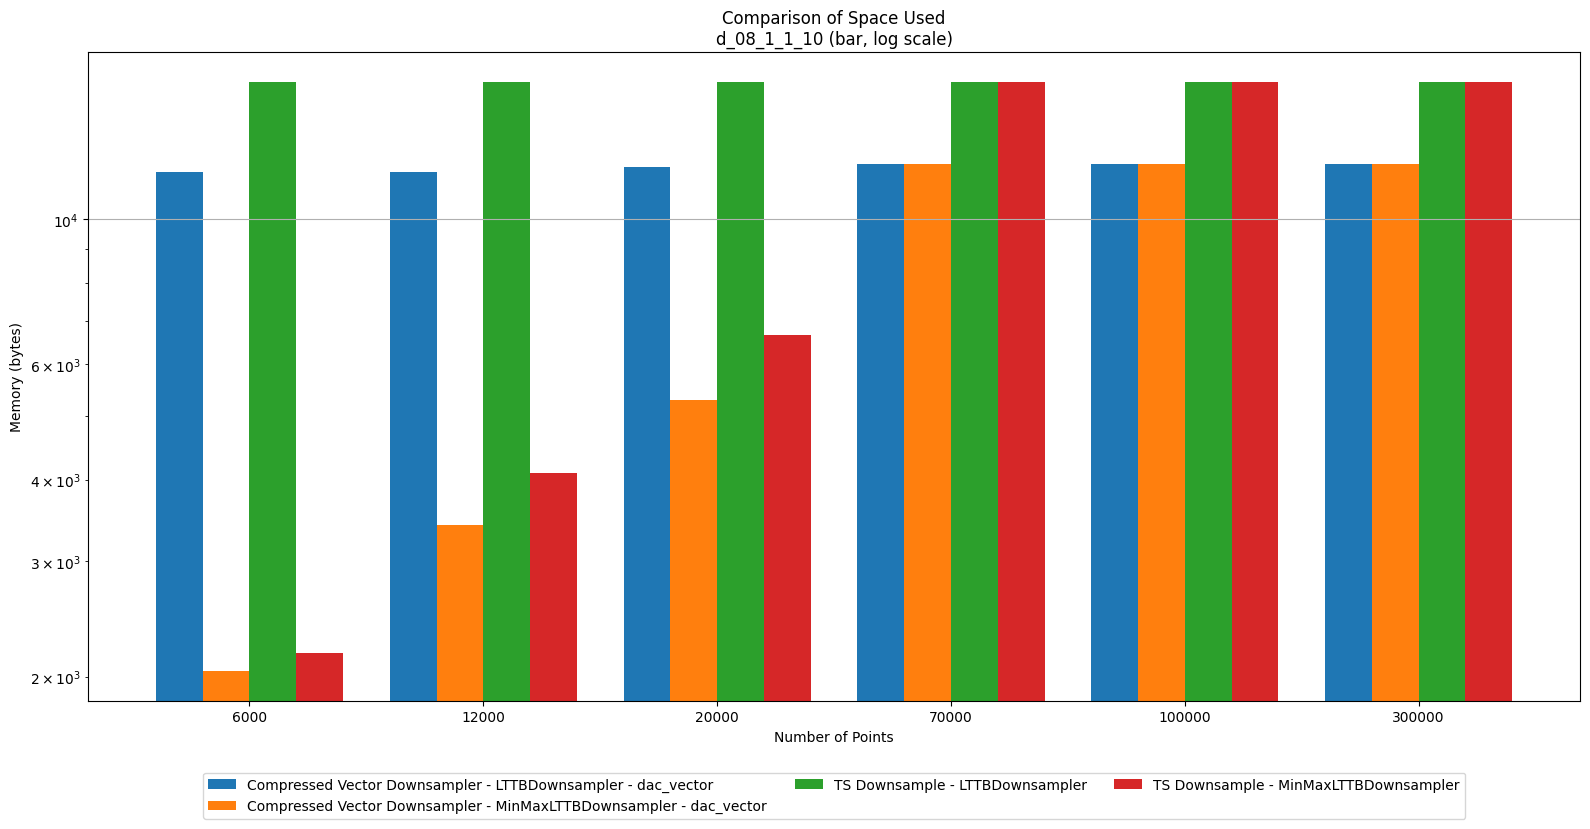
\includegraphics[width=1\textwidth]{anexo/exp/Comparison of Space Used/bar_plots/Comparison of Space Used_d_08_1_1_10_log_bar.png}
        \caption[]{Gráfico de espacio usado por las diferentes bibliotecas para el input \textbf{d\_08\_1\_1\_10}.}
        \label{fig:comparison_of_space_used_plot_bar_2}
    \end{figure}
}

\DeclareRobustCommand{\ComparisonOfSpaceUsedThreePlotLine}{
    %insertar imagen
    \begin{figure}[H]
        \centering
        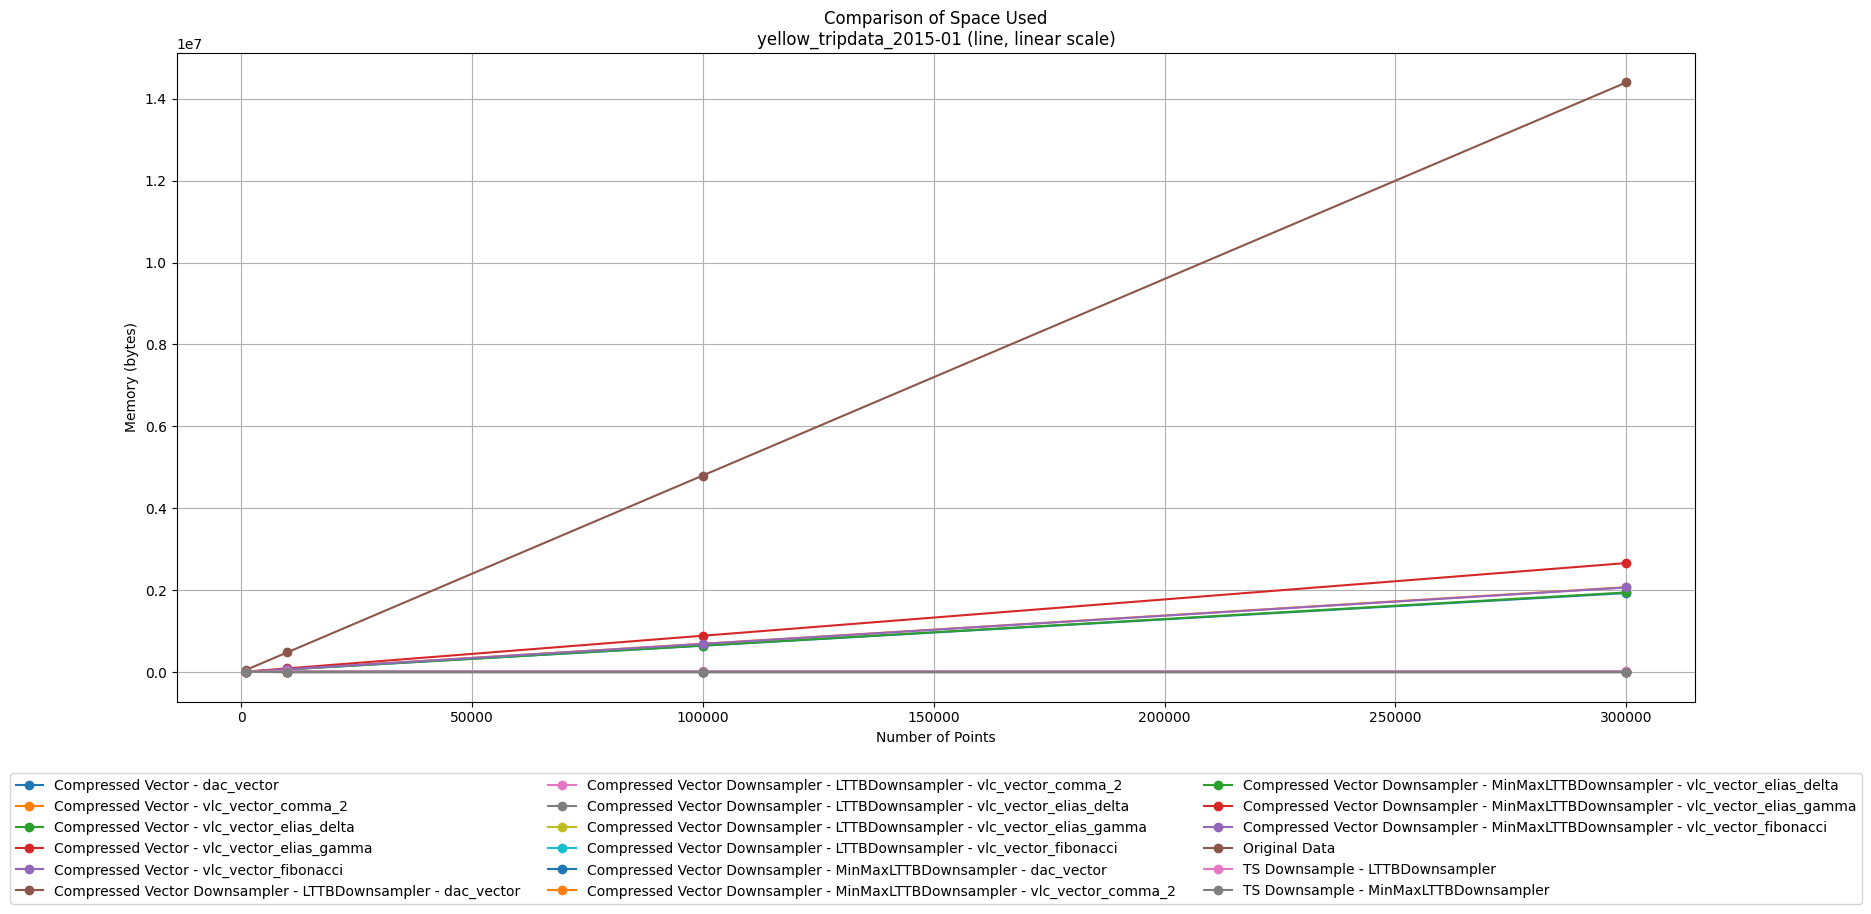
\includegraphics[width=1\textwidth]{anexo/exp/Comparison of Space Used/plots/Comparison of Space Used_yellow_tripdata_2015-01_linear_line.png}
        \caption[]{Gráfico de espacio usado por las diferentes bibliotecas para el input \textbf{yellow\_tripdata\_2015\_01}.}
        \label{fig:comparison_of_space_used_plot_line_3}
    \end{figure}
}

\DeclareRobustCommand{\ComparisonOfSpaceUsedThreePlotBar}{
    %insertar imagen
    \begin{figure}[H]
        \centering
        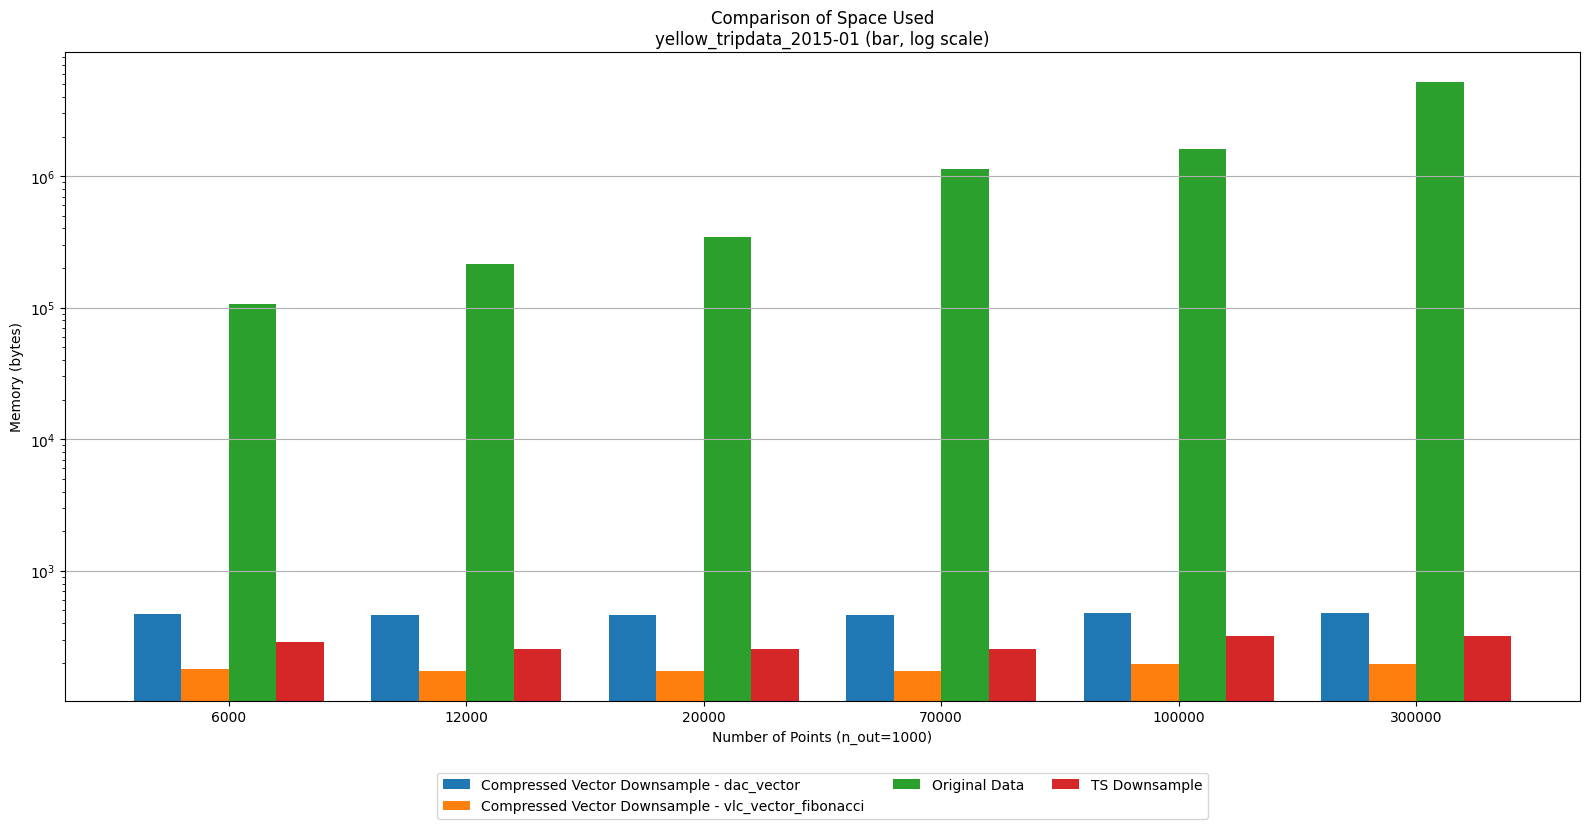
\includegraphics[width=1\textwidth]{anexo/exp/Comparison of Space Used/bar_plots/Comparison of Space Used_yellow_tripdata_2015-01_log_bar.png}
        \caption[]{Gráfico de espacio usado por las diferentes bibliotecas para el input \textbf{yellow\_tripdata\_2015\_01}.}
        \label{fig:comparison_of_space_used_plot_bar_3}
    \end{figure}
}



% ===========================
% CVD Decimal Places Access Time Comparison
% ===========================
\DeclareRobustCommand{\CVDDecimalPlacesAccessTimeComparisonOnePlotLine}{
    \begin{figure}[H]
        \centering
        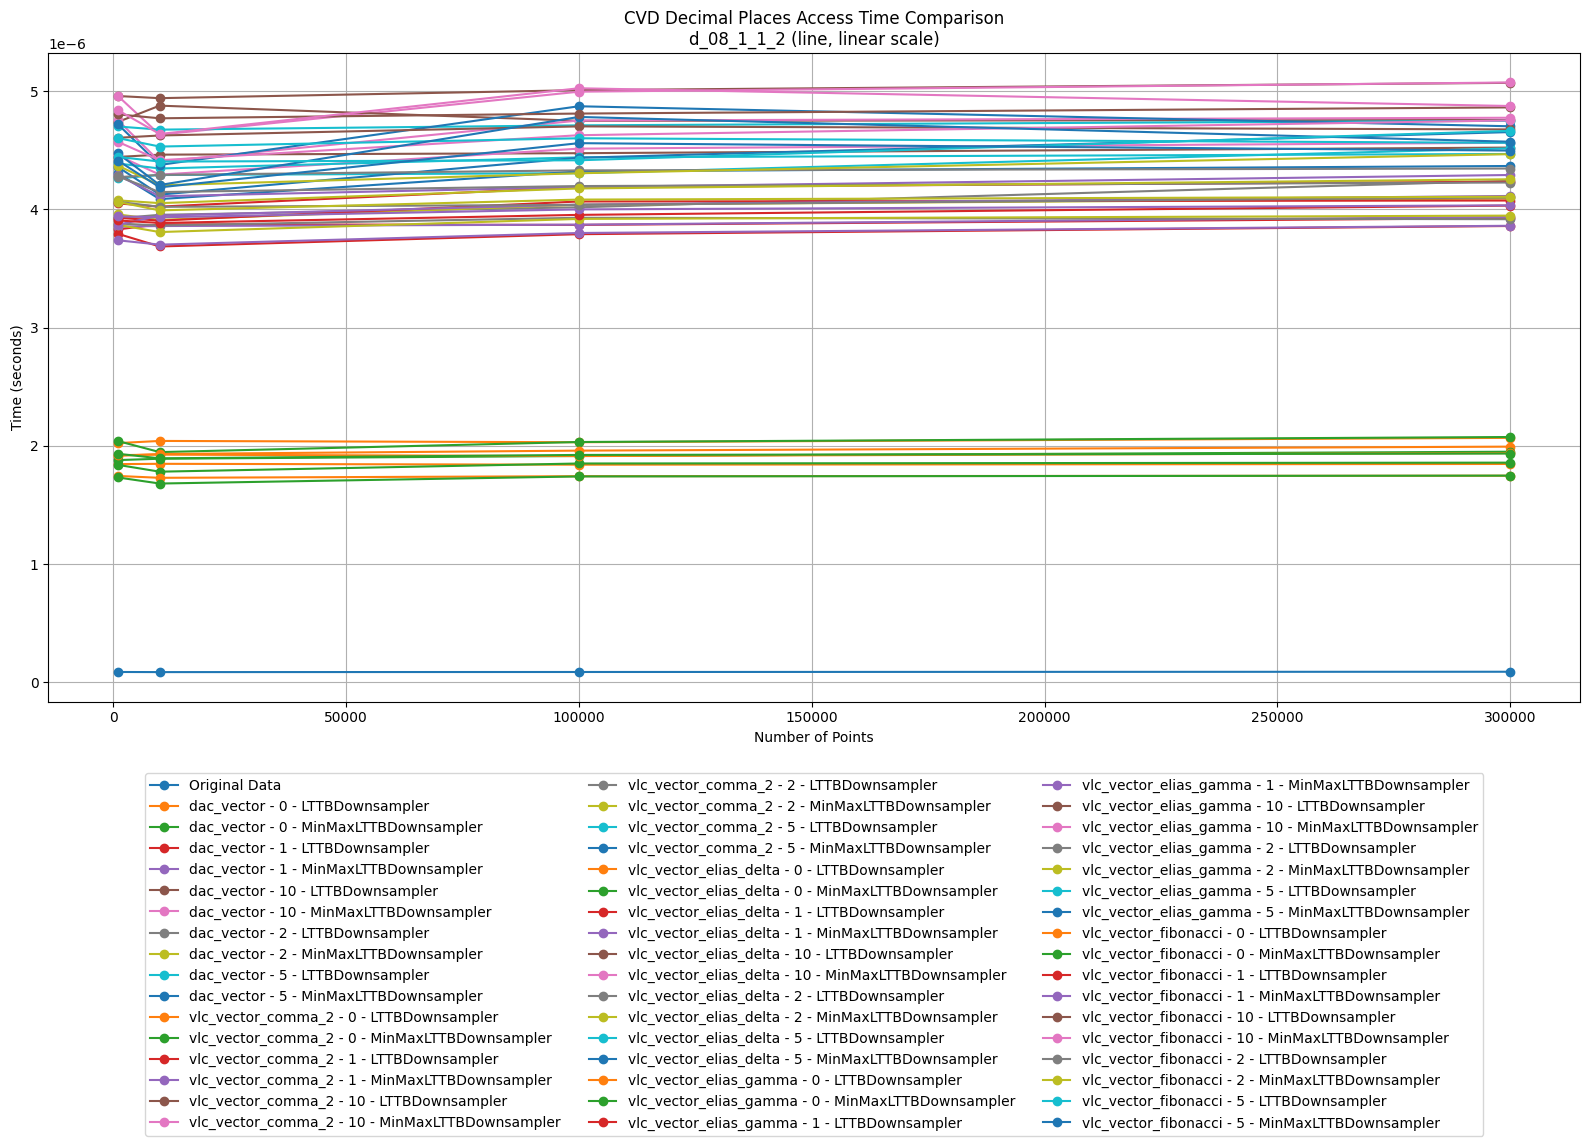
\includegraphics[width=1\textwidth]{anexo/exp/CVD Decimal Places Access Time Comparison/plots/CVD Decimal Places Access Time Comparison_d_08_1_1_2_linear_line.png}
        \caption[]{Gráfico de tiempo de acceso CVD con diferentes lugares decimales para el input \textbf{d\_08\_1\_1\_2}.}
        \label{fig:cvd_decimal_places_access_time_comparison_plot_line_1}
    \end{figure}
    \begin{figure}[H]
        \centering
        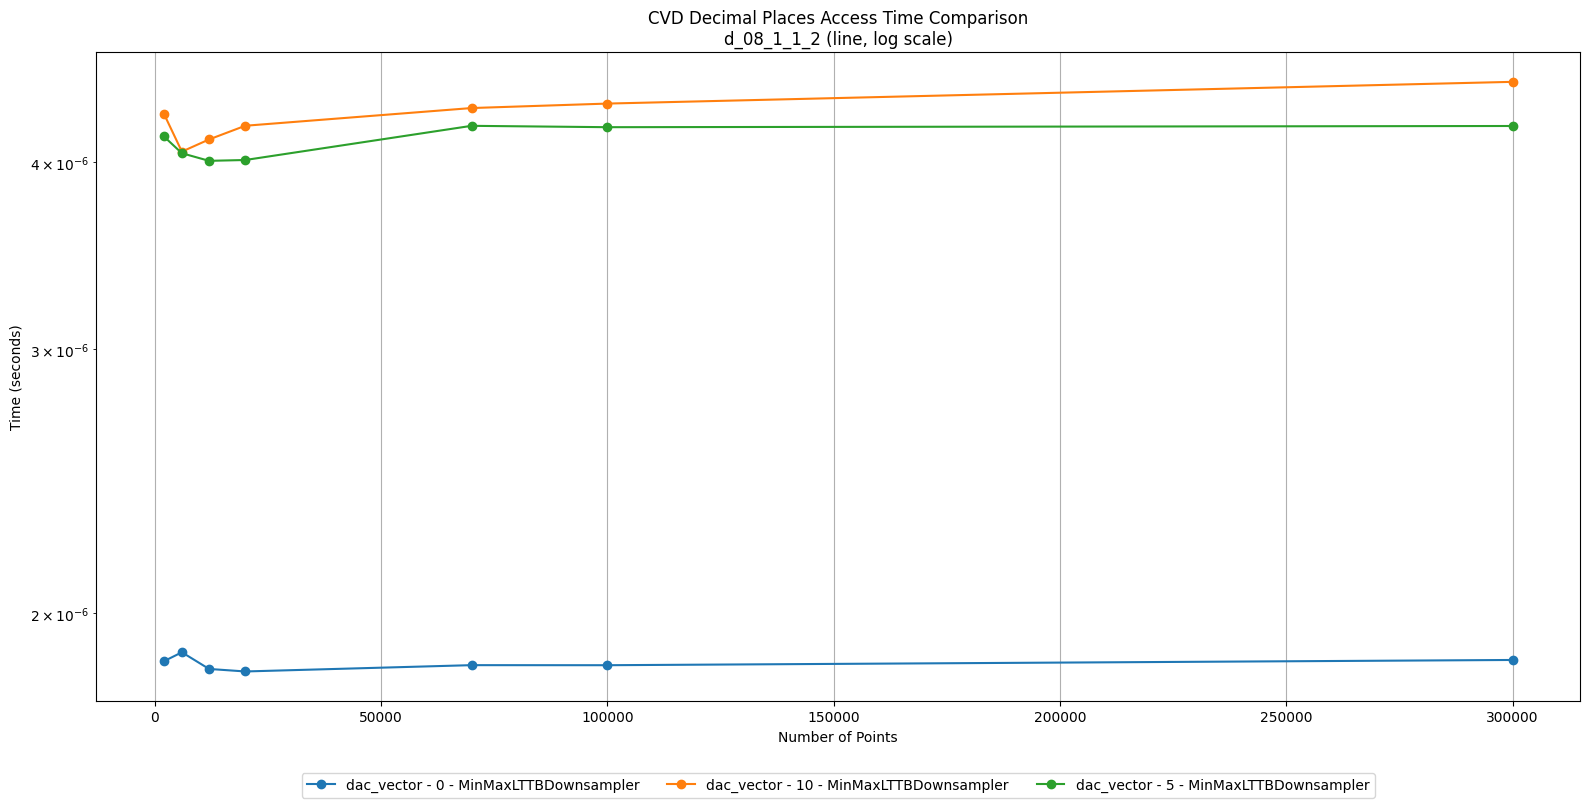
\includegraphics[width=1\textwidth]{anexo/exp/CVD Decimal Places Access Time Comparison/plots/CVD Decimal Places Access Time Comparison_d_08_1_1_2_log_line.png}
        \caption[]{Gráfico de tiempo de acceso CVD con diferentes lugares decimales para el input \textbf{d\_08\_1\_1\_2} en escala logarítmica.}
        \label{fig:cvd_decimal_places_access_time_comparison_plot_log_1}
    \end{figure}
}

\DeclareRobustCommand{\CVDDecimalPlacesAccessTimeComparisonTwoPlotLine}{
    \begin{figure}[H]
        \centering
        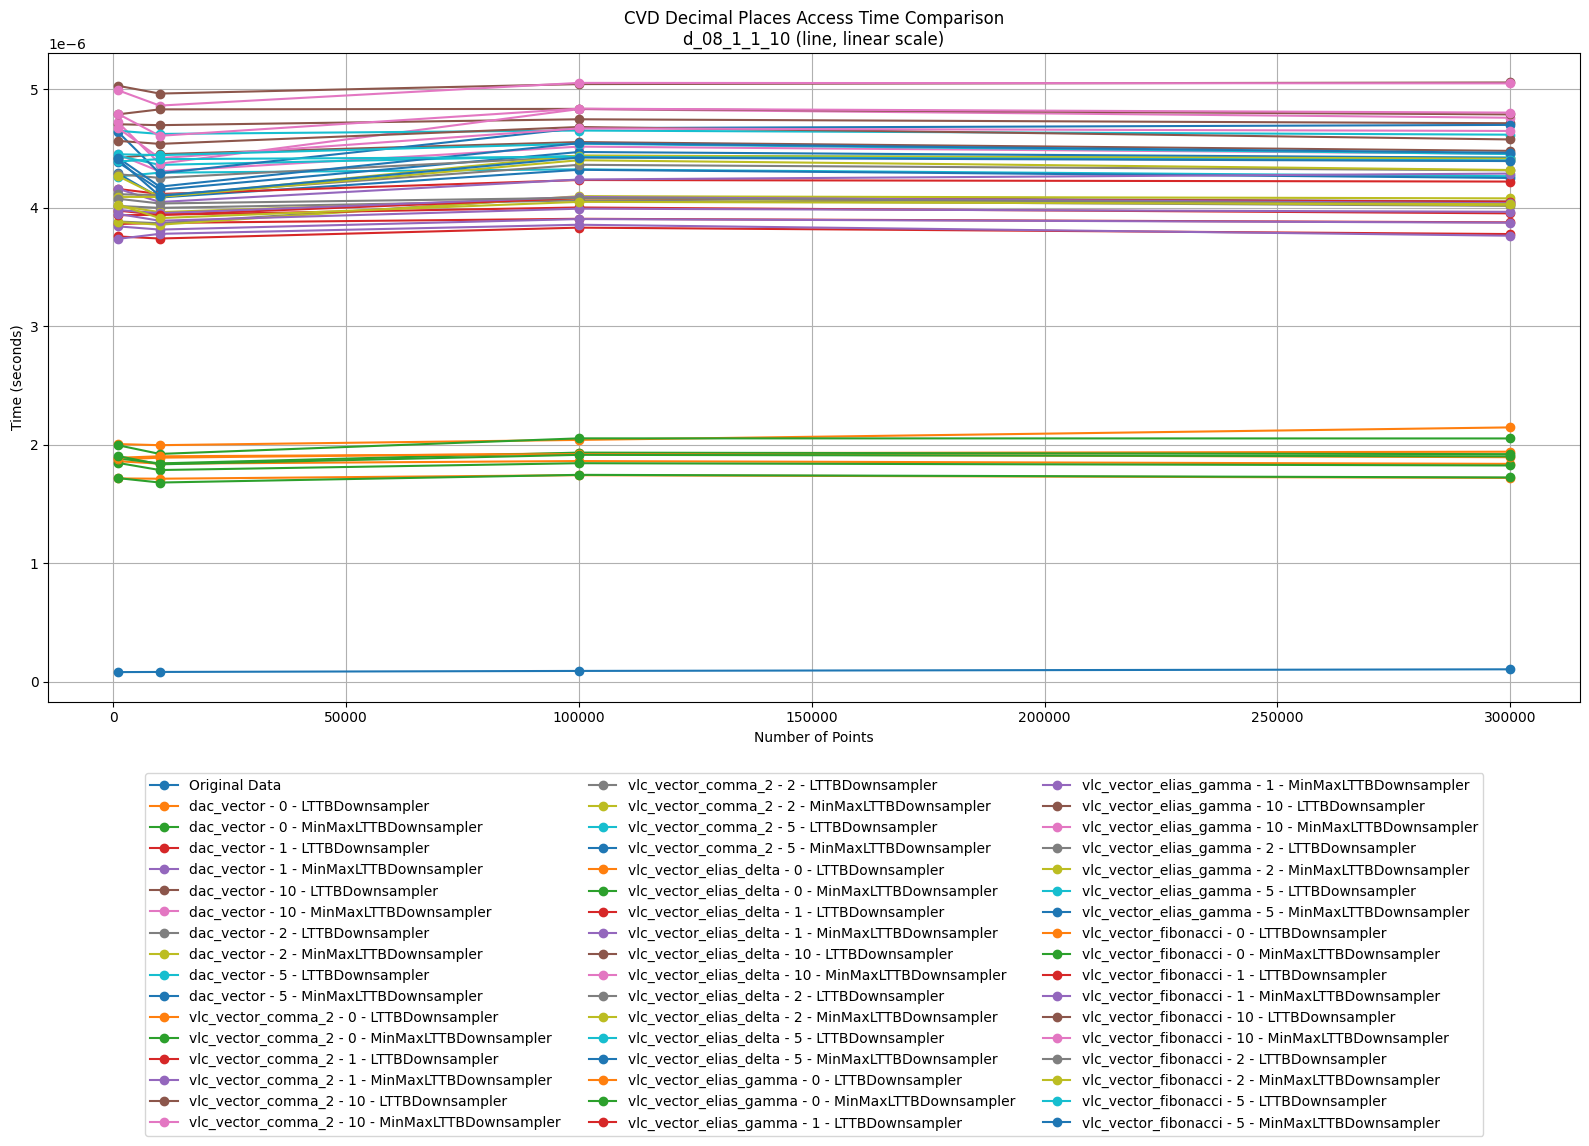
\includegraphics[width=1\textwidth]{anexo/exp/CVD Decimal Places Access Time Comparison/plots/CVD Decimal Places Access Time Comparison_d_08_1_1_10_linear_line.png}
        \caption[]{Gráfico de tiempo de acceso CVD con diferentes lugares decimales para el input \textbf{d\_08\_1\_1\_10}.}
        \label{fig:cvd_decimal_places_access_time_comparison_plot_line_2}
    \end{figure}
    \begin{figure}[H]
        \centering
        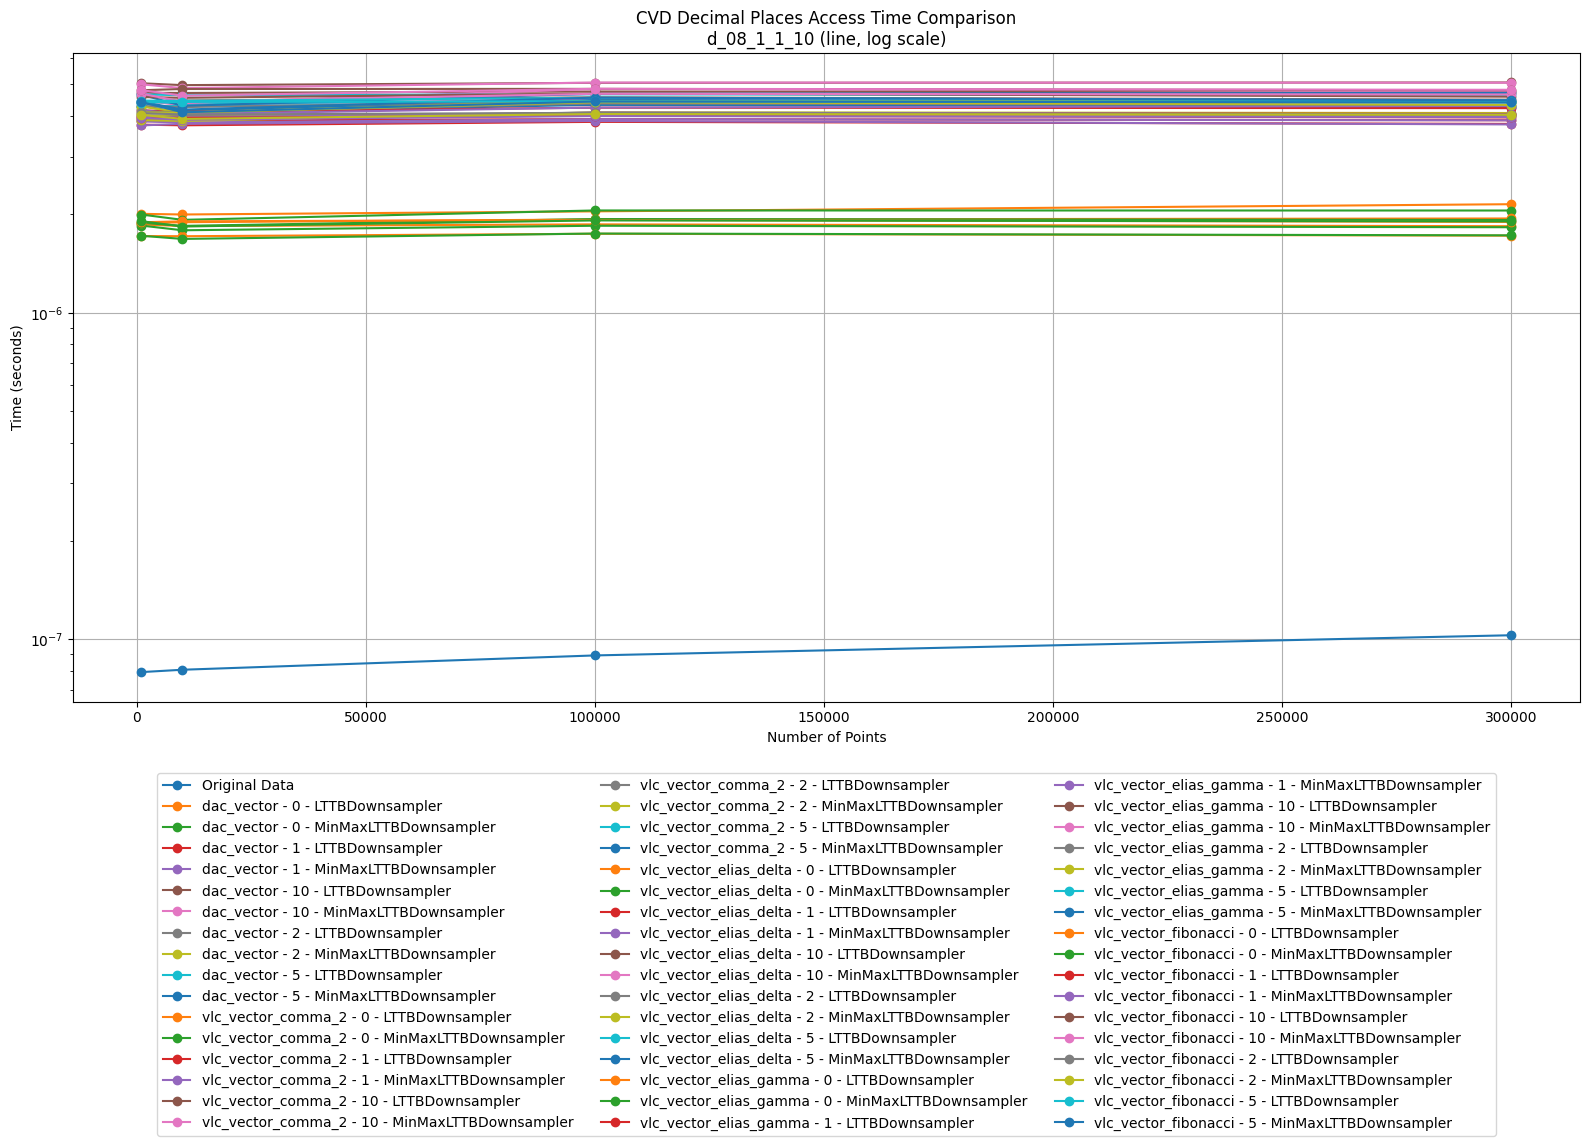
\includegraphics[width=1\textwidth]{anexo/exp/CVD Decimal Places Access Time Comparison/plots/CVD Decimal Places Access Time Comparison_d_08_1_1_10_log_line.png}
        \caption[]{Gráfico de tiempo de acceso CVD con diferentes lugares decimales para el input \textbf{d\_08\_1\_1\_10} en escala logarítmica.}
        \label{fig:cvd_decimal_places_access_time_comparison_plot_log_2}
    \end{figure}
}

\DeclareRobustCommand{\CVDDecimalPlacesAccessTimeComparisonThreePlotLine}{
    \begin{figure}[H]
        \centering
        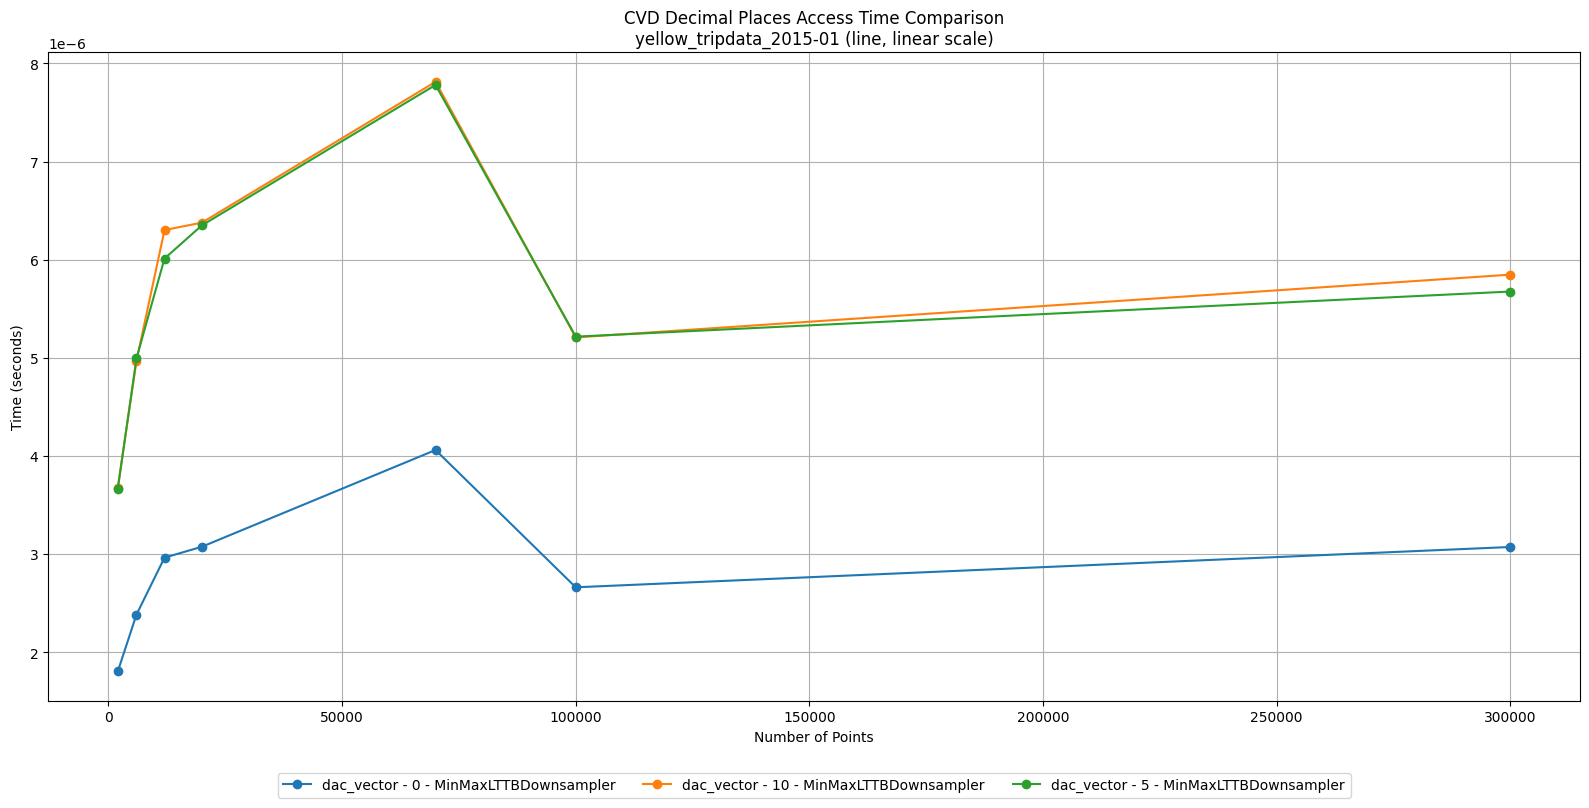
\includegraphics[width=1\textwidth]{anexo/exp/CVD Decimal Places Access Time Comparison/plots/CVD Decimal Places Access Time Comparison_yellow_tripdata_2015-01_linear_line.png}
        \caption[]{Gráfico de tiempo de acceso CVD con diferentes lugares decimales para el input \textbf{yellow\_tripdata\_2015\_01}.}
        \label{fig:cvd_decimal_places_access_time_comparison_plot_line_3}
    \end{figure}
    \begin{figure}[H]
        \centering
        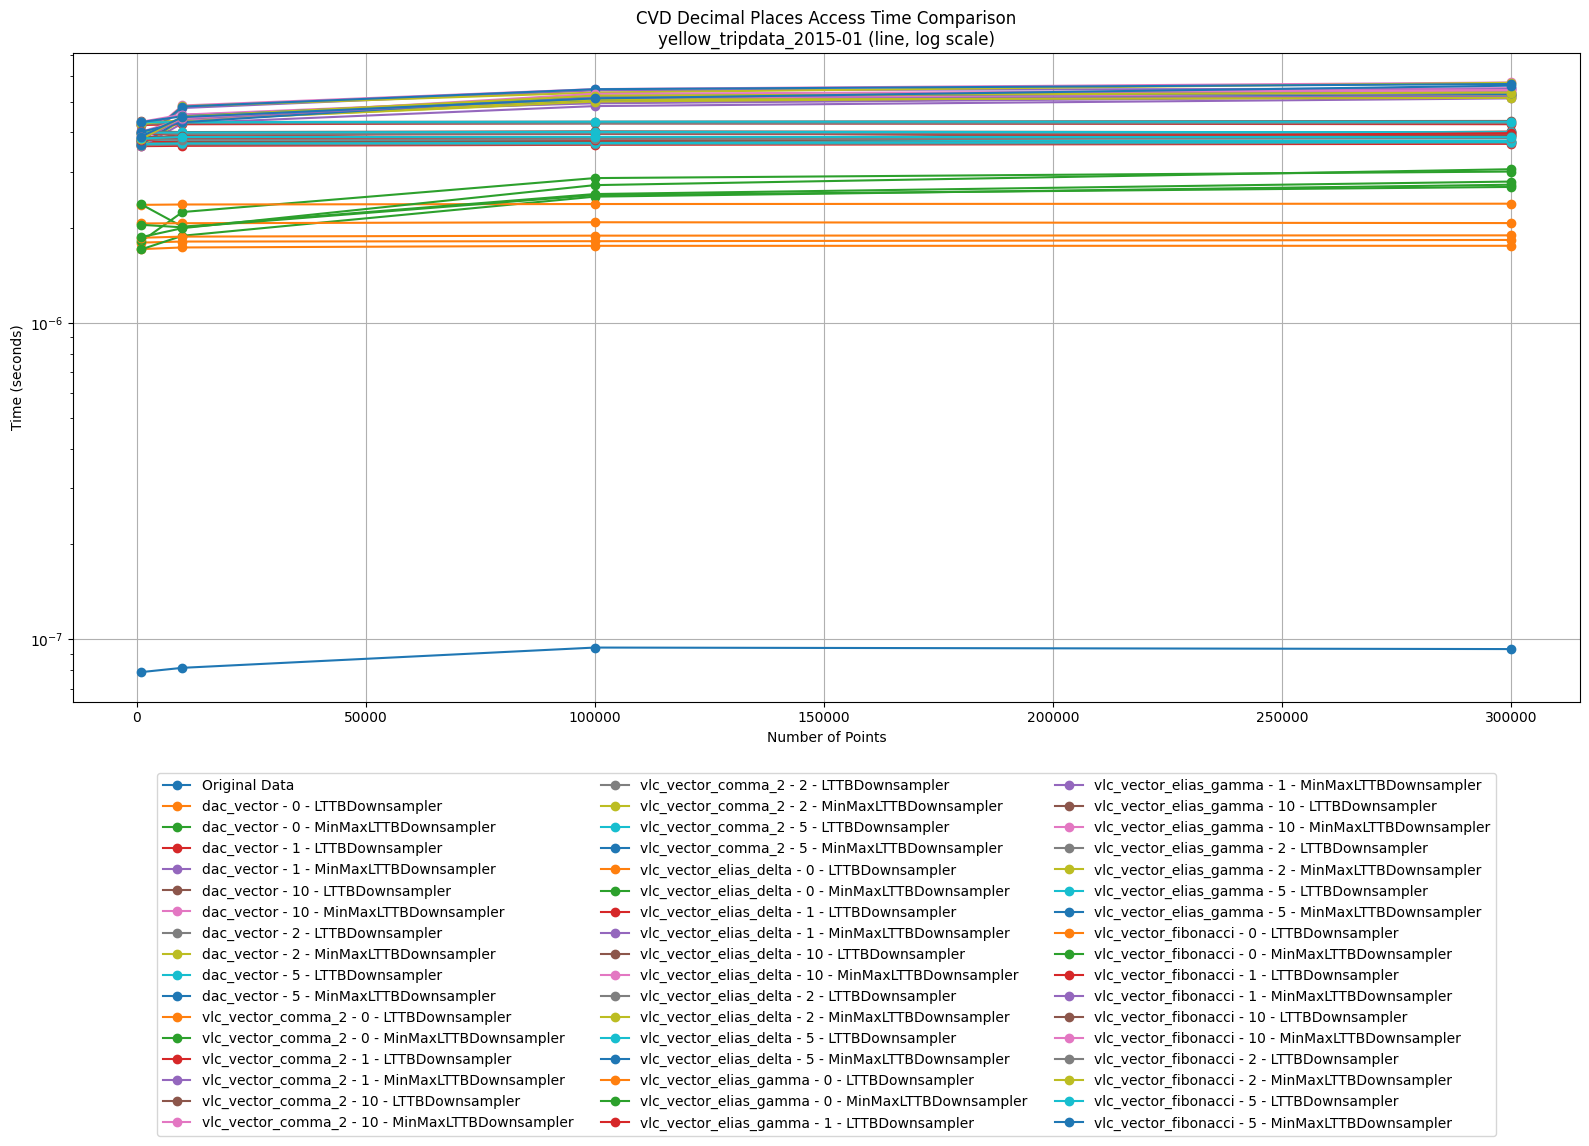
\includegraphics[width=1\textwidth]{anexo/exp/CVD Decimal Places Access Time Comparison/plots/CVD Decimal Places Access Time Comparison_yellow_tripdata_2015-01_log_line.png}
        \caption[]{Gráfico de tiempo de acceso CVD con diferentes lugares decimales para el input \textbf{yellow\_tripdata\_2015\_01} en escala logarítmica.}
        \label{fig:cvd_decimal_places_access_time_comparison_plot_log_3}
    \end{figure}
}


% ===========================
% CVD Decimal Places Build Time Comparison
% ===========================
\DeclareRobustCommand{\CVDDecimalPlacesBuildTimeComparisonOnePlotLine}{
    \begin{figure}[H]
        \centering
        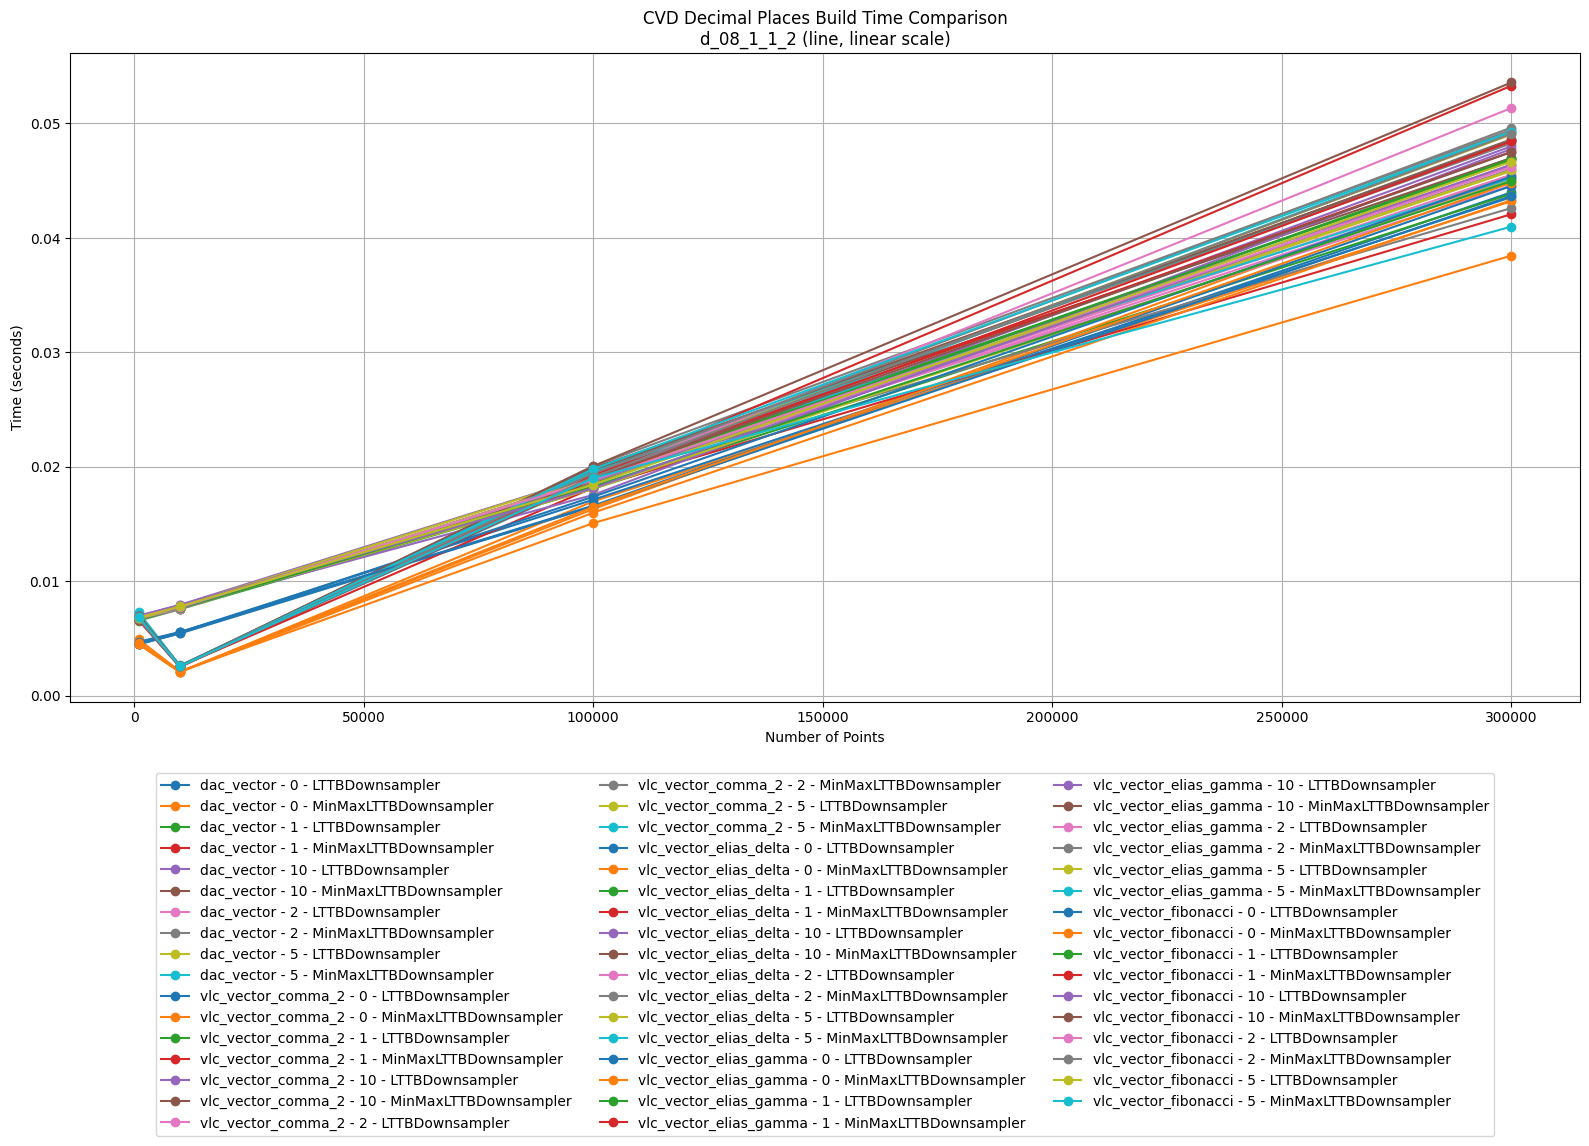
\includegraphics[width=1\textwidth]{anexo/exp/CVD Decimal Places Build Time Comparison/plots/CVD Decimal Places Build Time Comparison_d_08_1_1_2_linear_line.png}
        \caption[]{Gráfico de tiempo de construcción CVD con diferentes lugares decimales para el input \textbf{d\_08\_1\_1\_2}.}
        \label{fig:cvd_decimal_places_build_time_comparison_plot_line_1}
    \end{figure}
    \begin{figure}[H]
        \centering
        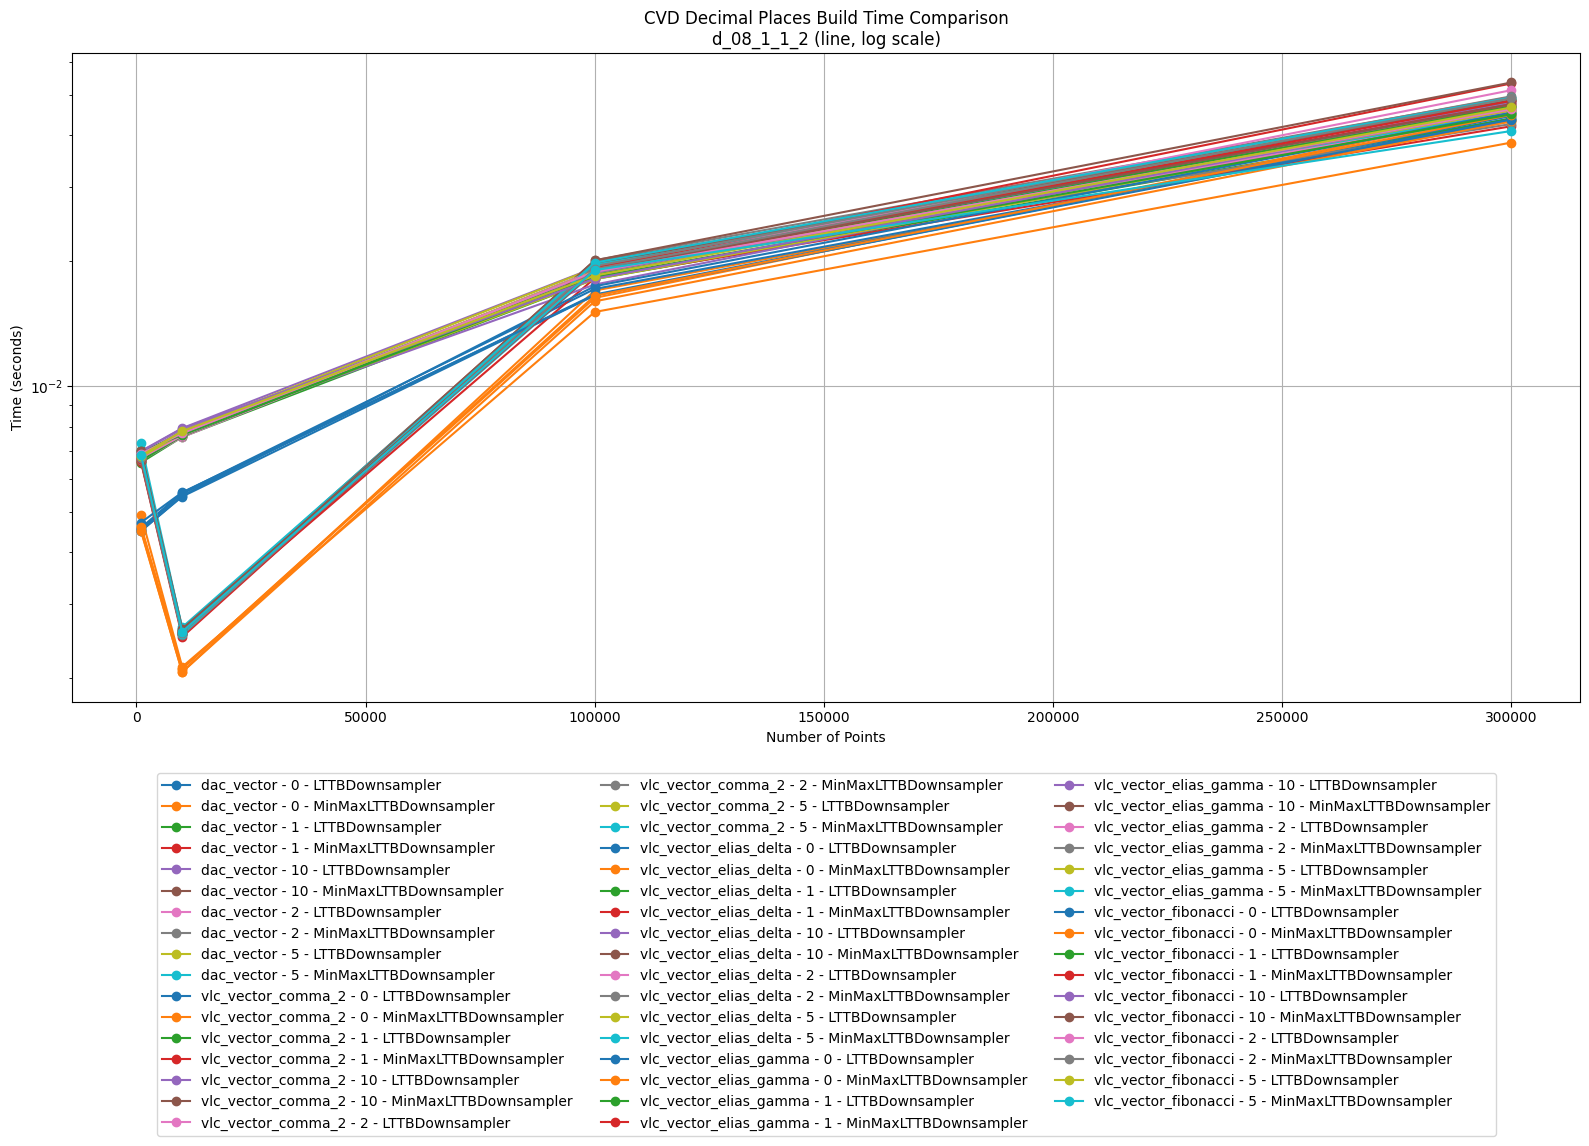
\includegraphics[width=1\textwidth]{anexo/exp/CVD Decimal Places Build Time Comparison/plots/CVD Decimal Places Build Time Comparison_d_08_1_1_2_log_line.png}
        \caption[]{Gráfico de tiempo de construcción CVD con diferentes lugares decimales para el input \textbf{d\_08\_1\_1\_2} en escala logarítmica.}
        \label{fig:cvd_decimal_places_build_time_comparison_plot_log_1}
    \end{figure}
}

\DeclareRobustCommand{\CVDDecimalPlacesBuildTimeComparisonTwoPlotLine}{
    \begin{figure}[H]
        \centering
        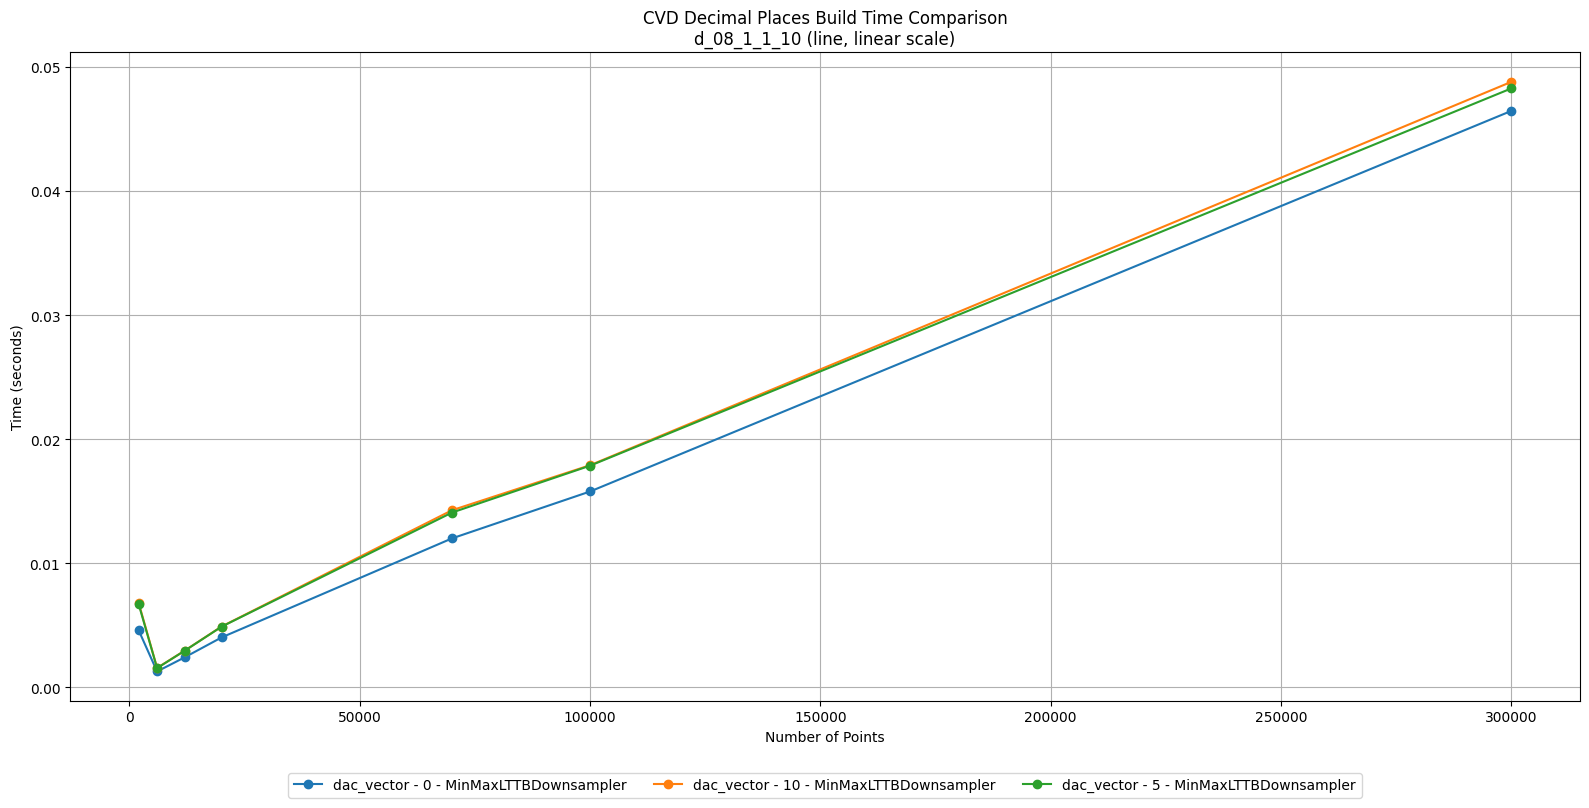
\includegraphics[width=1\textwidth]{anexo/exp/CVD Decimal Places Build Time Comparison/plots/CVD Decimal Places Build Time Comparison_d_08_1_1_10_linear_line.png}
        \caption[]{Gráfico de tiempo de construcción CVD con diferentes lugares decimales para el input \textbf{d\_08\_1\_1\_10}.}
        \label{fig:cvd_decimal_places_build_time_comparison_plot_line_2}
    \end{figure}
    \begin{figure}[H]
        \centering
        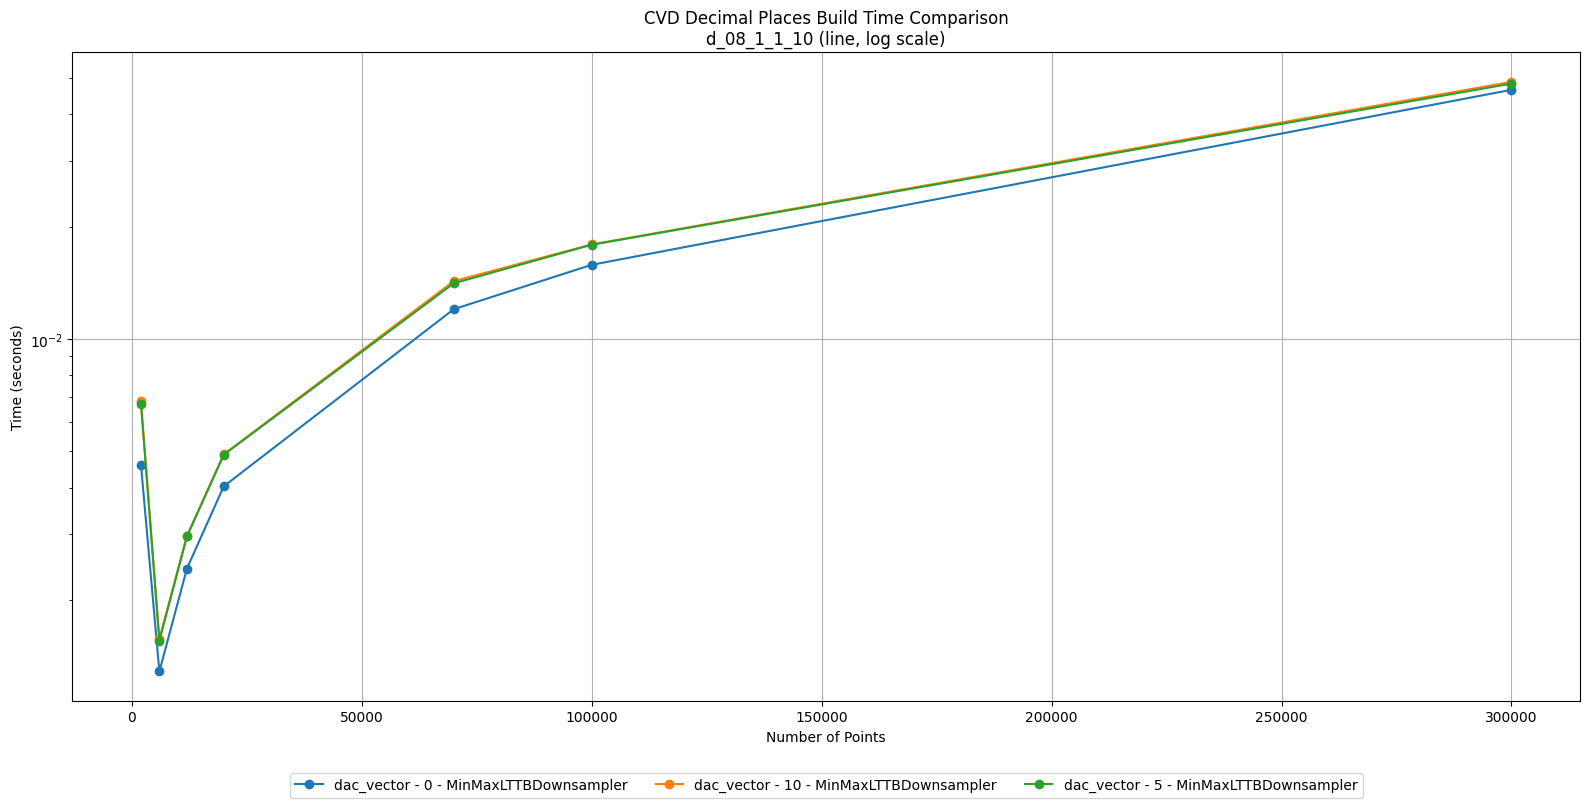
\includegraphics[width=1\textwidth]{anexo/exp/CVD Decimal Places Build Time Comparison/plots/CVD Decimal Places Build Time Comparison_d_08_1_1_10_log_line.png}
        \caption[]{Gráfico de tiempo de construcción CVD con diferentes lugares decimales para el input \textbf{d\_08\_1\_1\_10} en escala logarítmica.}
        \label{fig:cvd_decimal_places_build_time_comparison_plot_log_2}
    \end{figure}
}

\DeclareRobustCommand{\CVDDecimalPlacesBuildTimeComparisonThreePlotLine}{
    \begin{figure}[H]
        \centering
        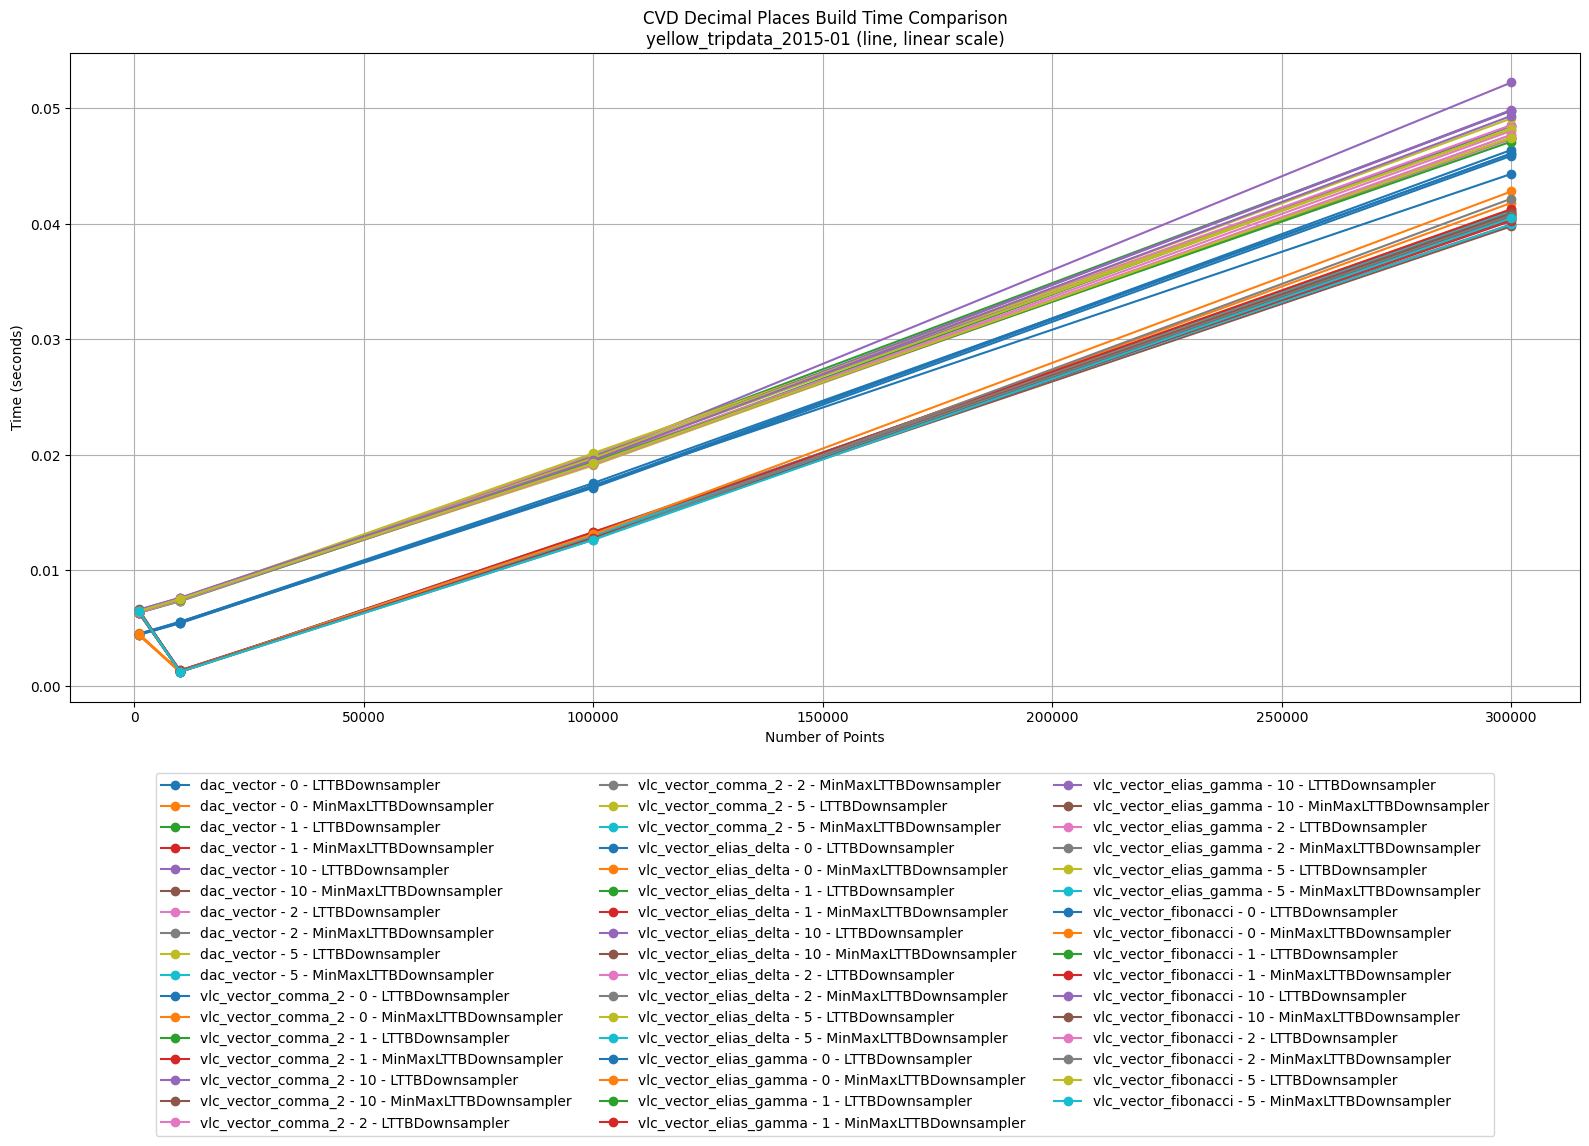
\includegraphics[width=1\textwidth]{anexo/exp/CVD Decimal Places Build Time Comparison/plots/CVD Decimal Places Build Time Comparison_yellow_tripdata_2015-01_linear_line.png}
        \caption[]{Gráfico de tiempo de construcción CVD con diferentes lugares decimales para el input \textbf{yellow\_tripdata\_2015\_01}.}
        \label{fig:cvd_decimal_places_build_time_comparison_plot_line_3}
    \end{figure}
    \begin{figure}[H]
        \centering
        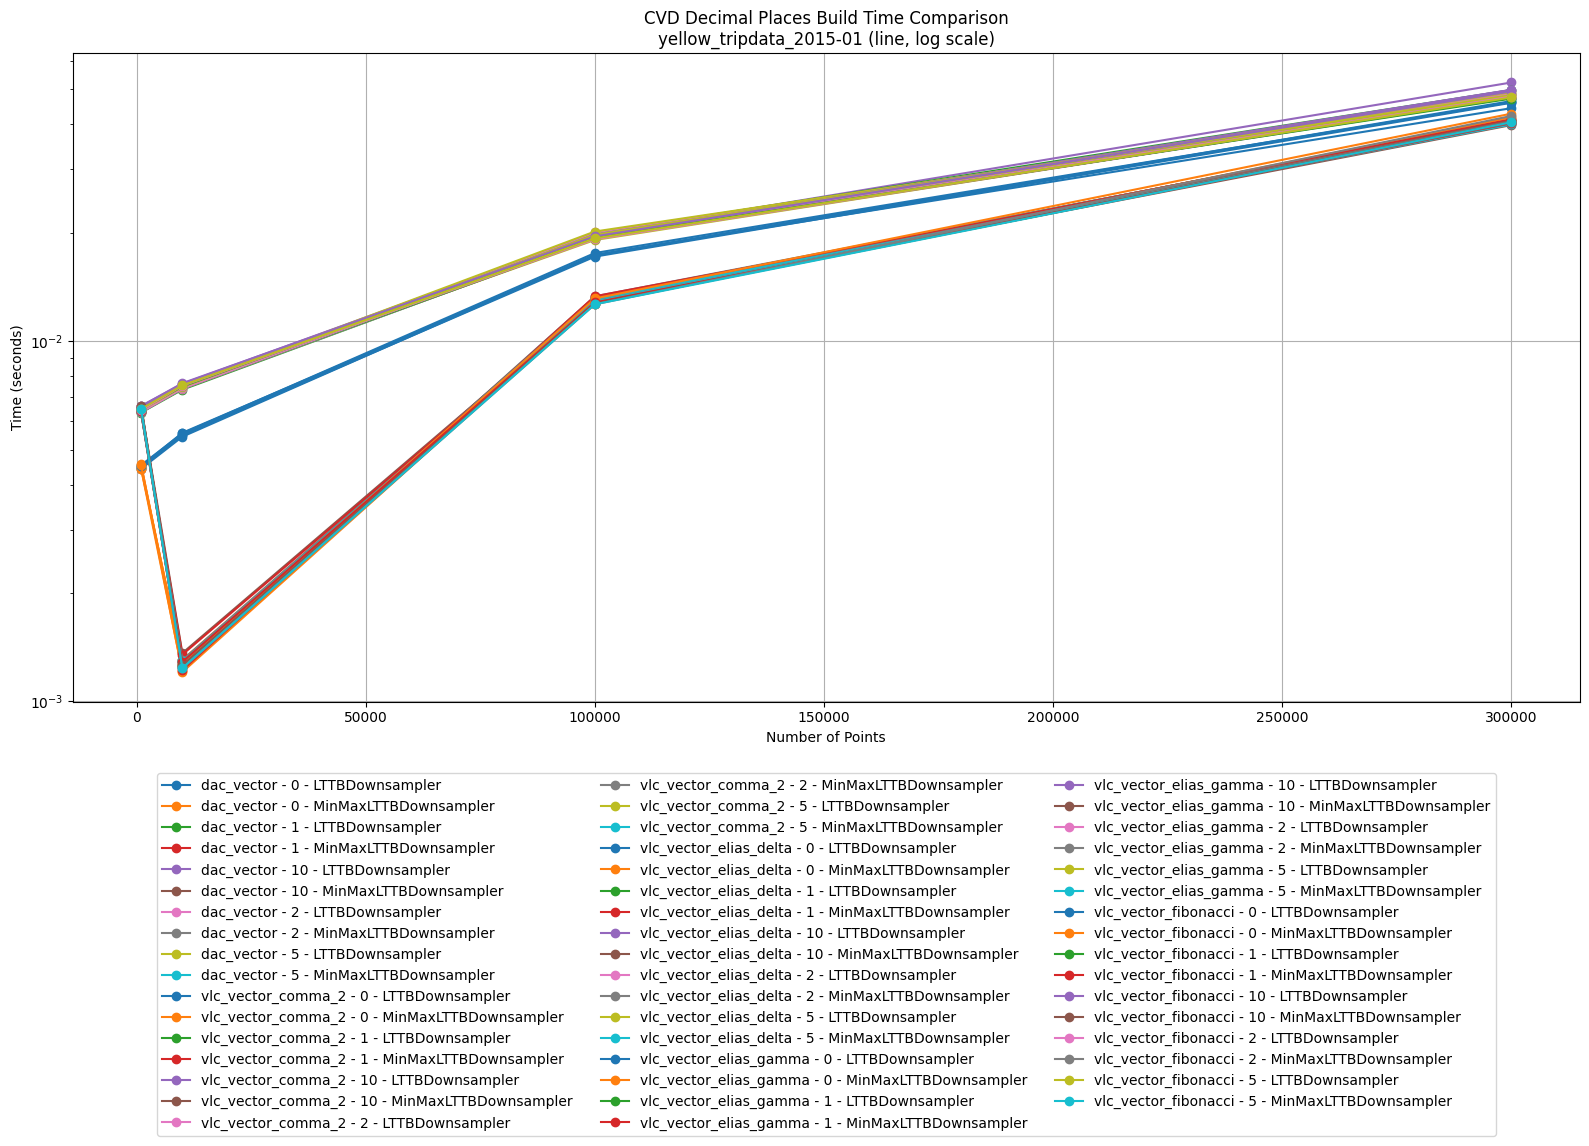
\includegraphics[width=1\textwidth]{anexo/exp/CVD Decimal Places Build Time Comparison/plots/CVD Decimal Places Build Time Comparison_yellow_tripdata_2015-01_log_line.png}
        \caption[]{Gráfico de tiempo de construcción CVD con diferentes lugares decimales para el input \textbf{yellow\_tripdata\_2015\_01} en escala logarítmica.}
        \label{fig:cvd_decimal_places_build_time_comparison_plot_log_3}
    \end{figure}
}


% ===========================
% CVD Decimal Places Size Comparison
% ===========================
\DeclareRobustCommand{\CVDDecimalPlacesSizeComparisonOnePlotLine}{
    \begin{figure}[H]
        \centering
        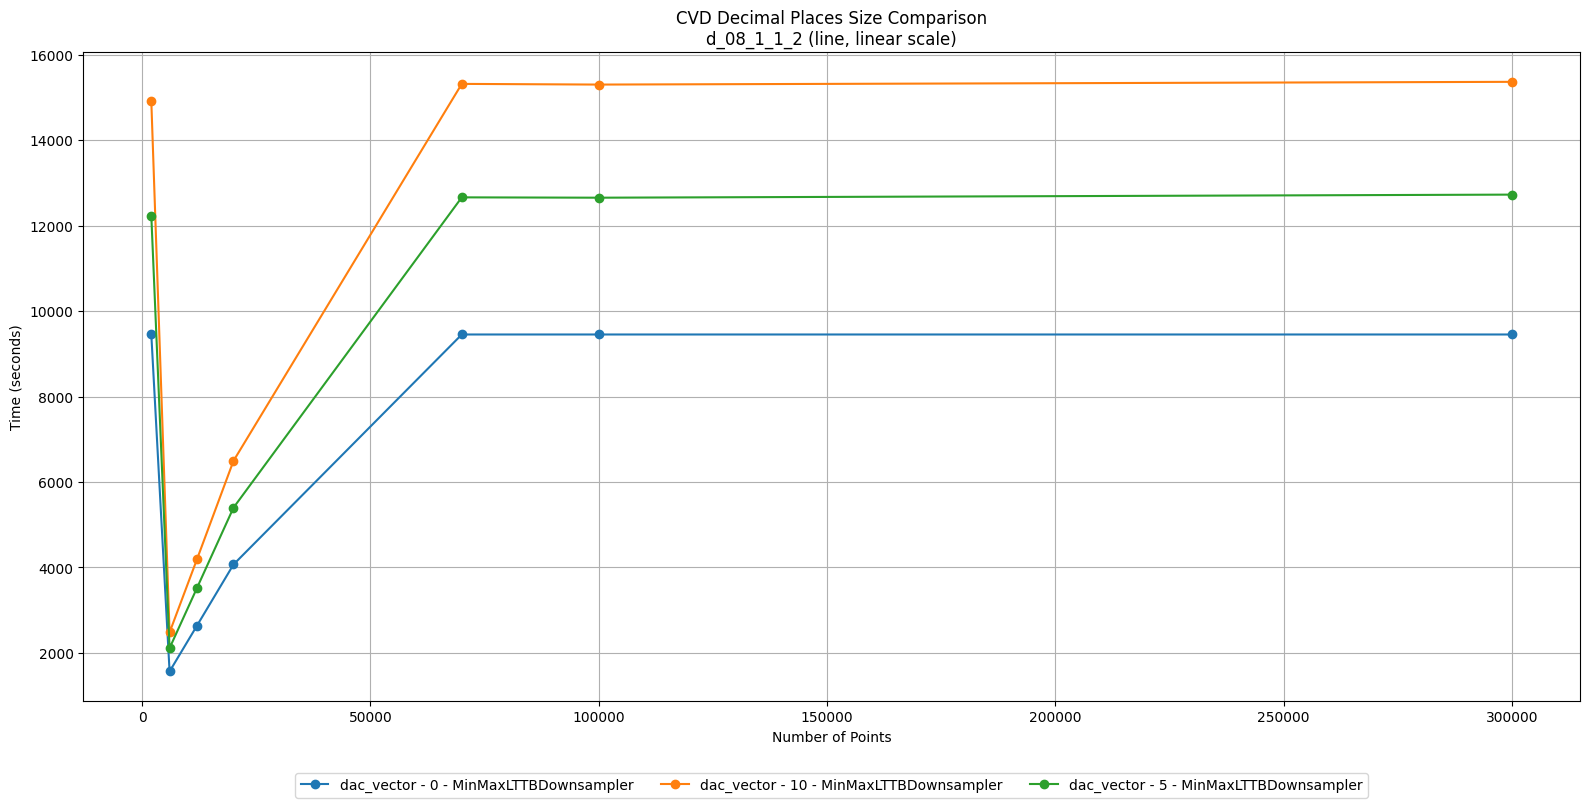
\includegraphics[width=1\textwidth]{anexo/exp/CVD Decimal Places Size Comparison/plots/CVD Decimal Places Size Comparison_d_08_1_1_2_linear_line.png}
        \caption[]{Gráfico de tamaño CVD con diferentes lugares decimales para el input \textbf{d\_08\_1\_1\_2}.}
        \label{fig:cvd_decimal_places_size_comparison_plot_line_1}
    \end{figure}
    \begin{figure}[H]
        \centering
        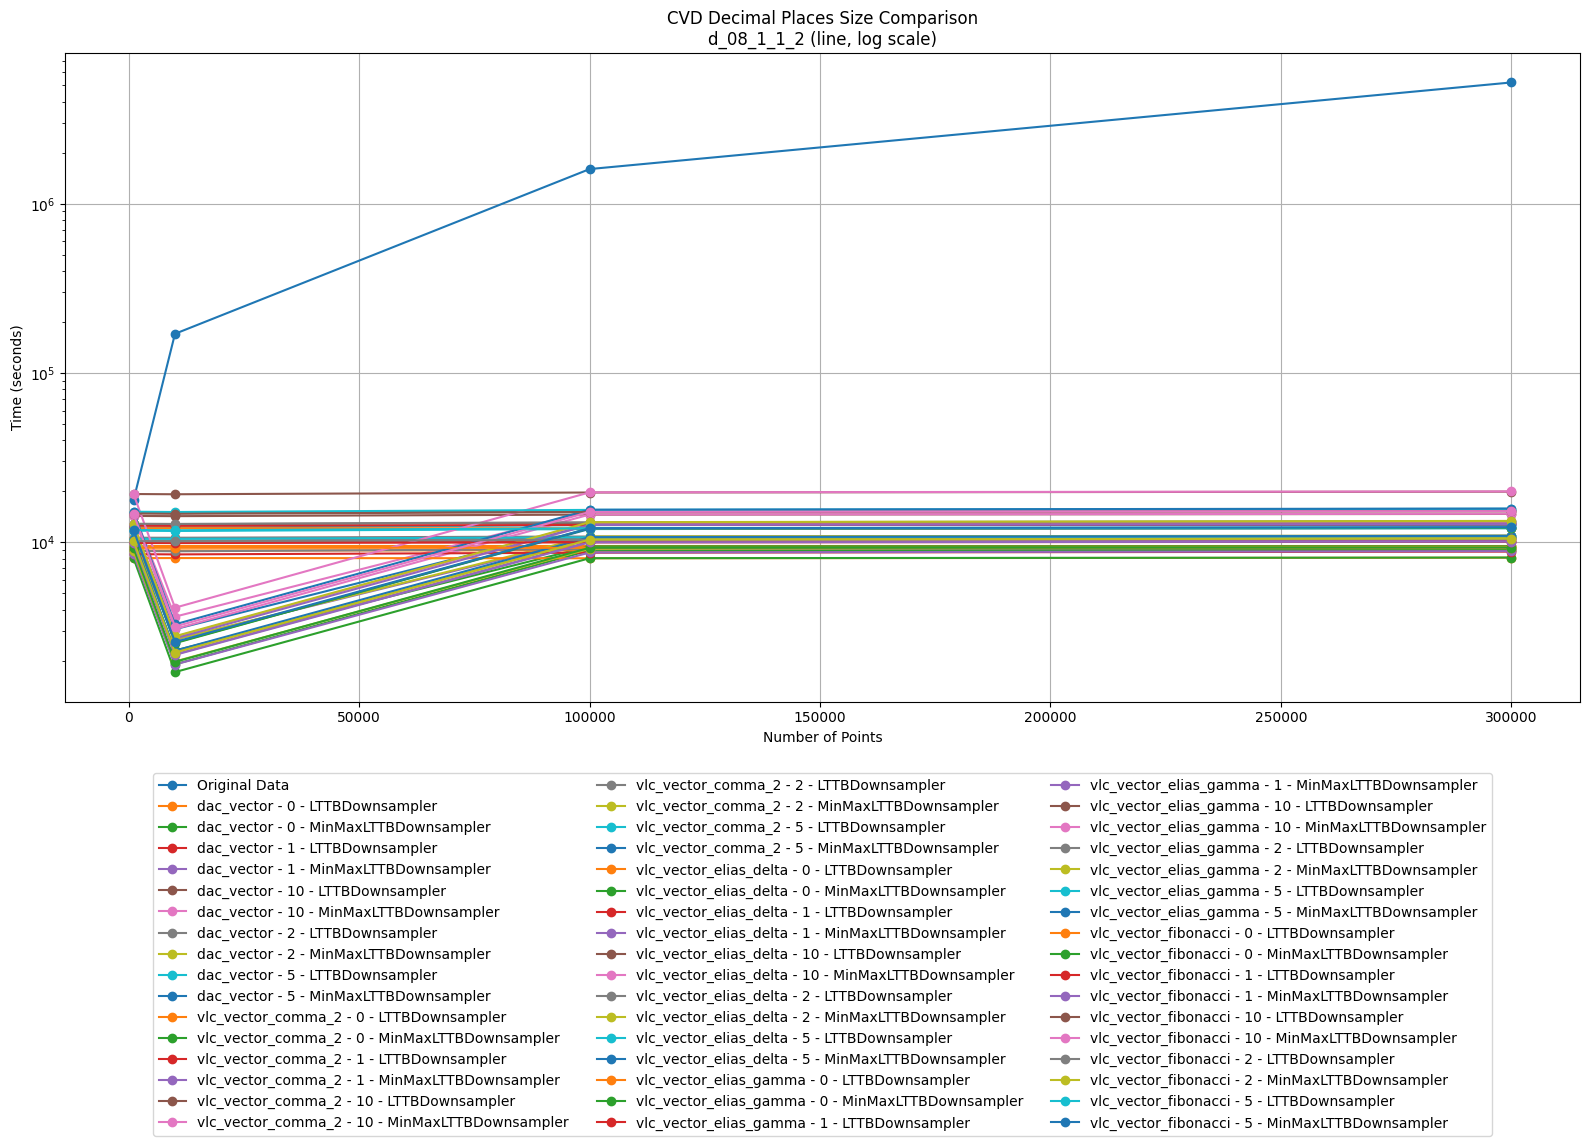
\includegraphics[width=1\textwidth]{anexo/exp/CVD Decimal Places Size Comparison/plots/CVD Decimal Places Size Comparison_d_08_1_1_2_log_line.png}
        \caption[]{Gráfico de tamaño CVD con diferentes lugares decimales para el input \textbf{d\_08\_1\_1\_2} en escala logarítmica.}
        \label{fig:cvd_decimal_places_size_comparison_plot_log_1}
    \end{figure}
}

\DeclareRobustCommand{\CVDDecimalPlacesSizeComparisonTwoPlotLine}{
    \begin{figure}[H]
        \centering
        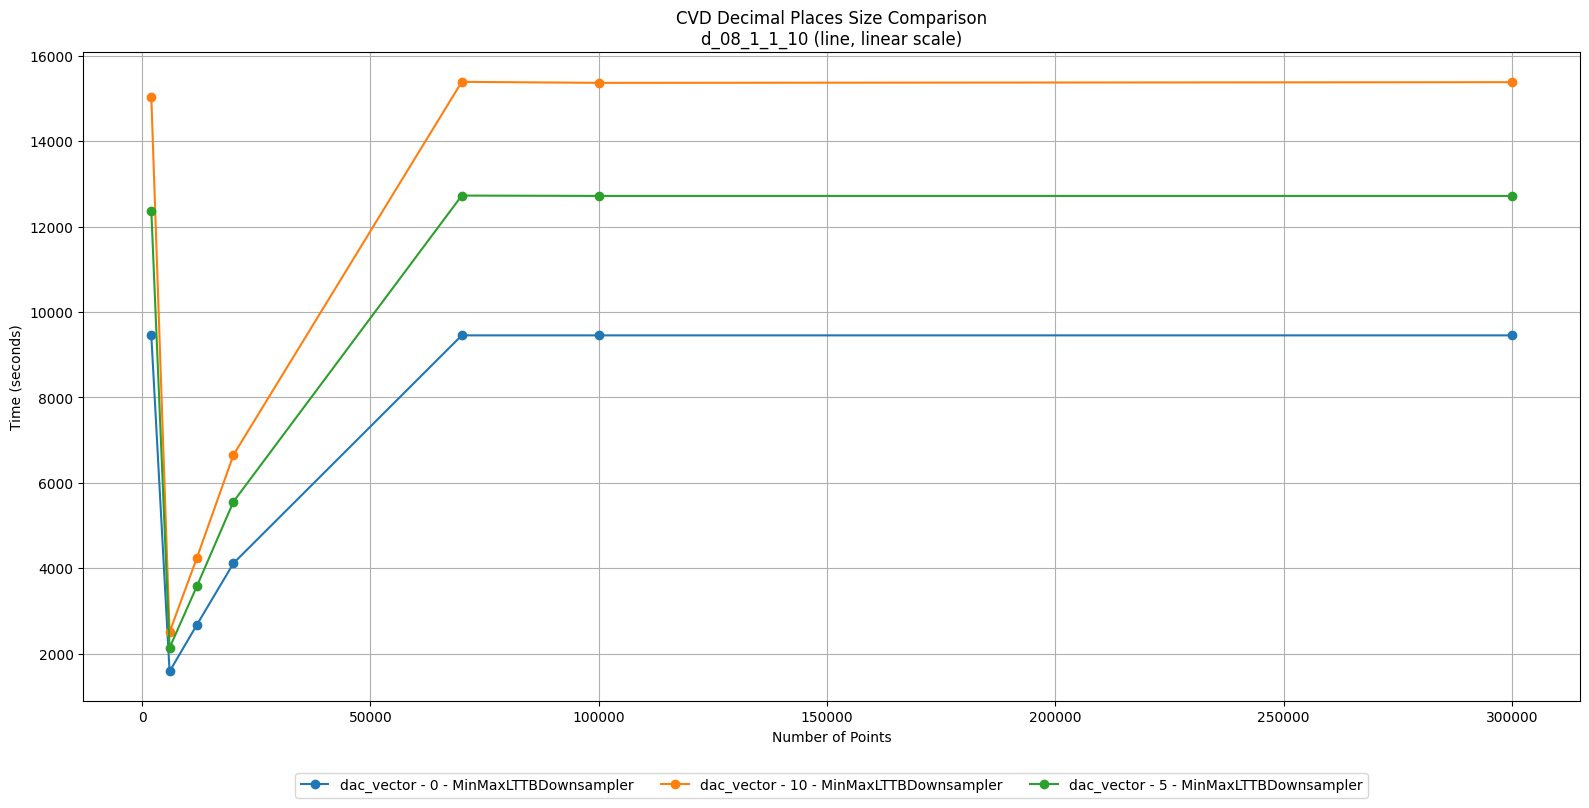
\includegraphics[width=1\textwidth]{anexo/exp/CVD Decimal Places Size Comparison/plots/CVD Decimal Places Size Comparison_d_08_1_1_10_linear_line.png}
        \caption[]{Gráfico de tamaño CVD con diferentes lugares decimales para el input \textbf{d\_08\_1\_1\_10}.}
        \label{fig:cvd_decimal_places_size_comparison_plot_line_2}
    \end{figure}
    \begin{figure}[H]
        \centering
        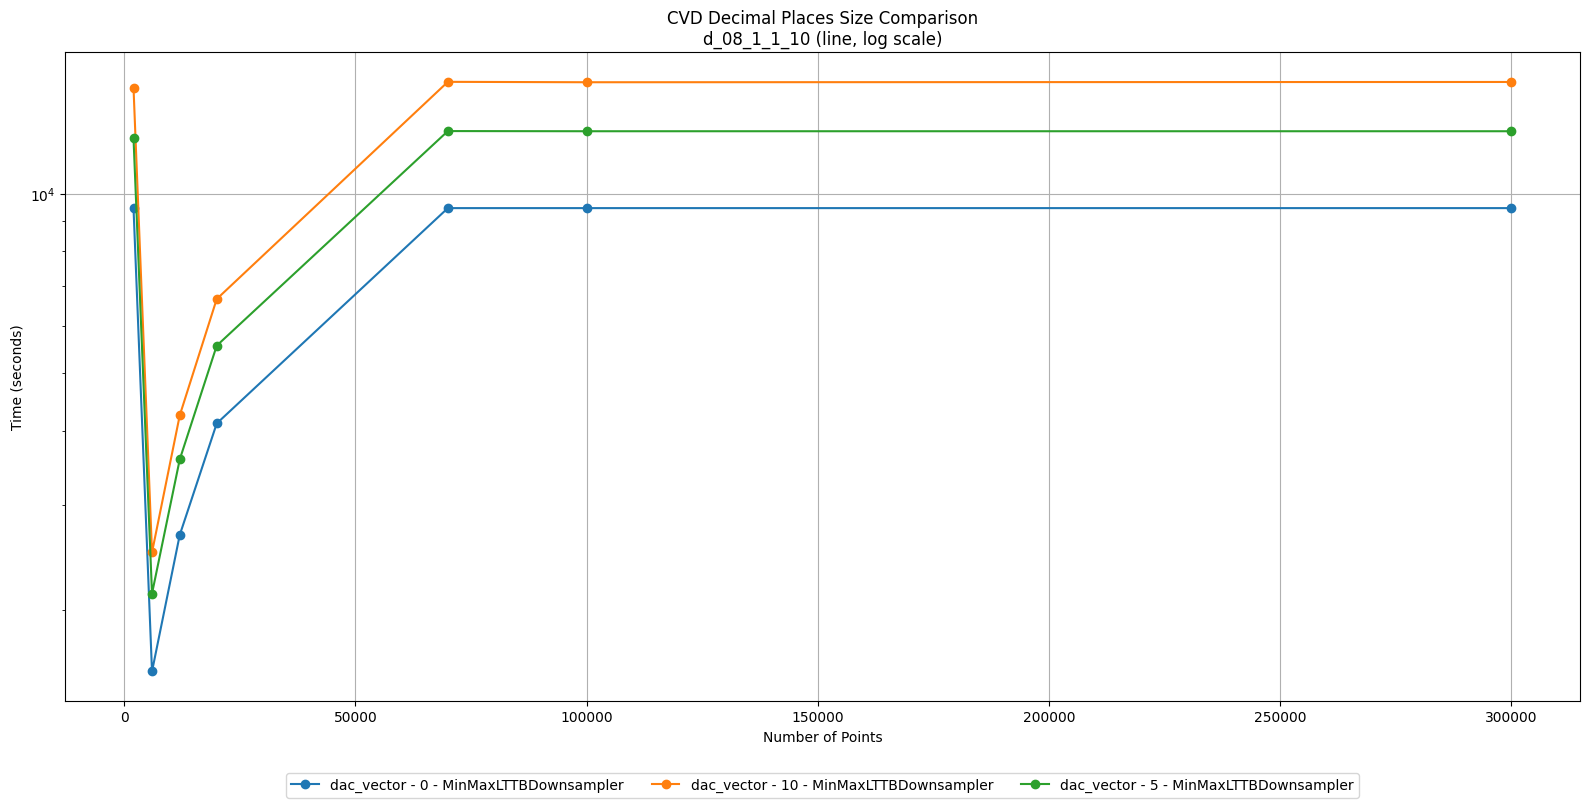
\includegraphics[width=1\textwidth]{anexo/exp/CVD Decimal Places Size Comparison/plots/CVD Decimal Places Size Comparison_d_08_1_1_10_log_line.png}
        \caption[]{Gráfico de tamaño CVD con diferentes lugares decimales para el input \textbf{d\_08\_1\_1\_10} en escala logarítmica.}
        \label{fig:cvd_decimal_places_size_comparison_plot_log_2}
    \end{figure}
}

\DeclareRobustCommand{\CVDDecimalPlacesSizeComparisonThreePlotLine}{
    \begin{figure}[H]
        \centering
        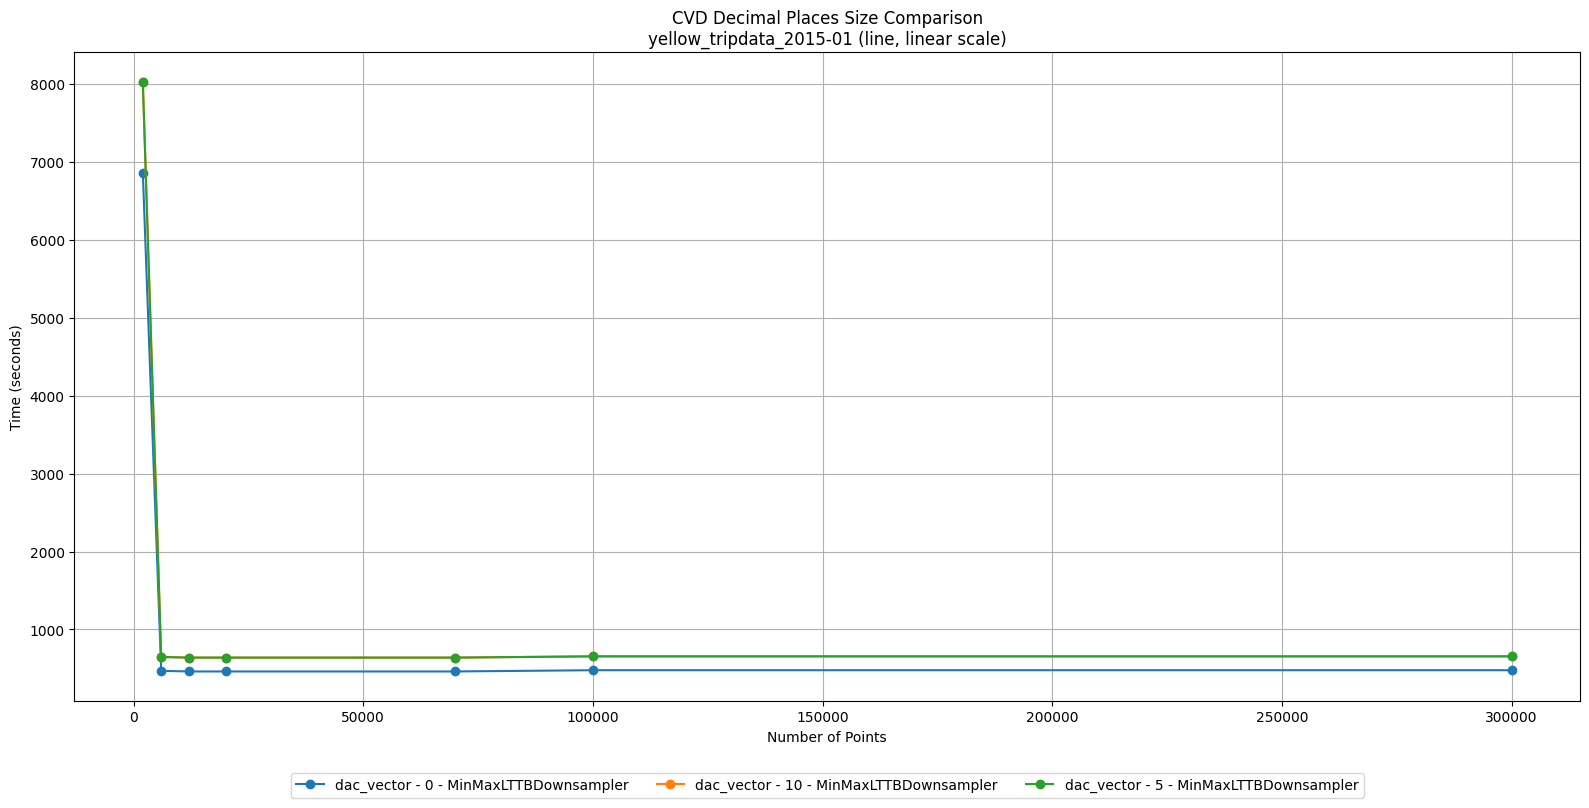
\includegraphics[width=1\textwidth]{anexo/exp/CVD Decimal Places Size Comparison/plots/CVD Decimal Places Size Comparison_yellow_tripdata_2015-01_linear_line.png}
        \caption[]{Gráfico de tamaño CVD con diferentes lugares decimales para el input \textbf{yellow\_tripdata\_2015\_01}.}
        \label{fig:cvd_decimal_places_size_comparison_plot_line_3}
    \end{figure}
    \begin{figure}[H]
        \centering
        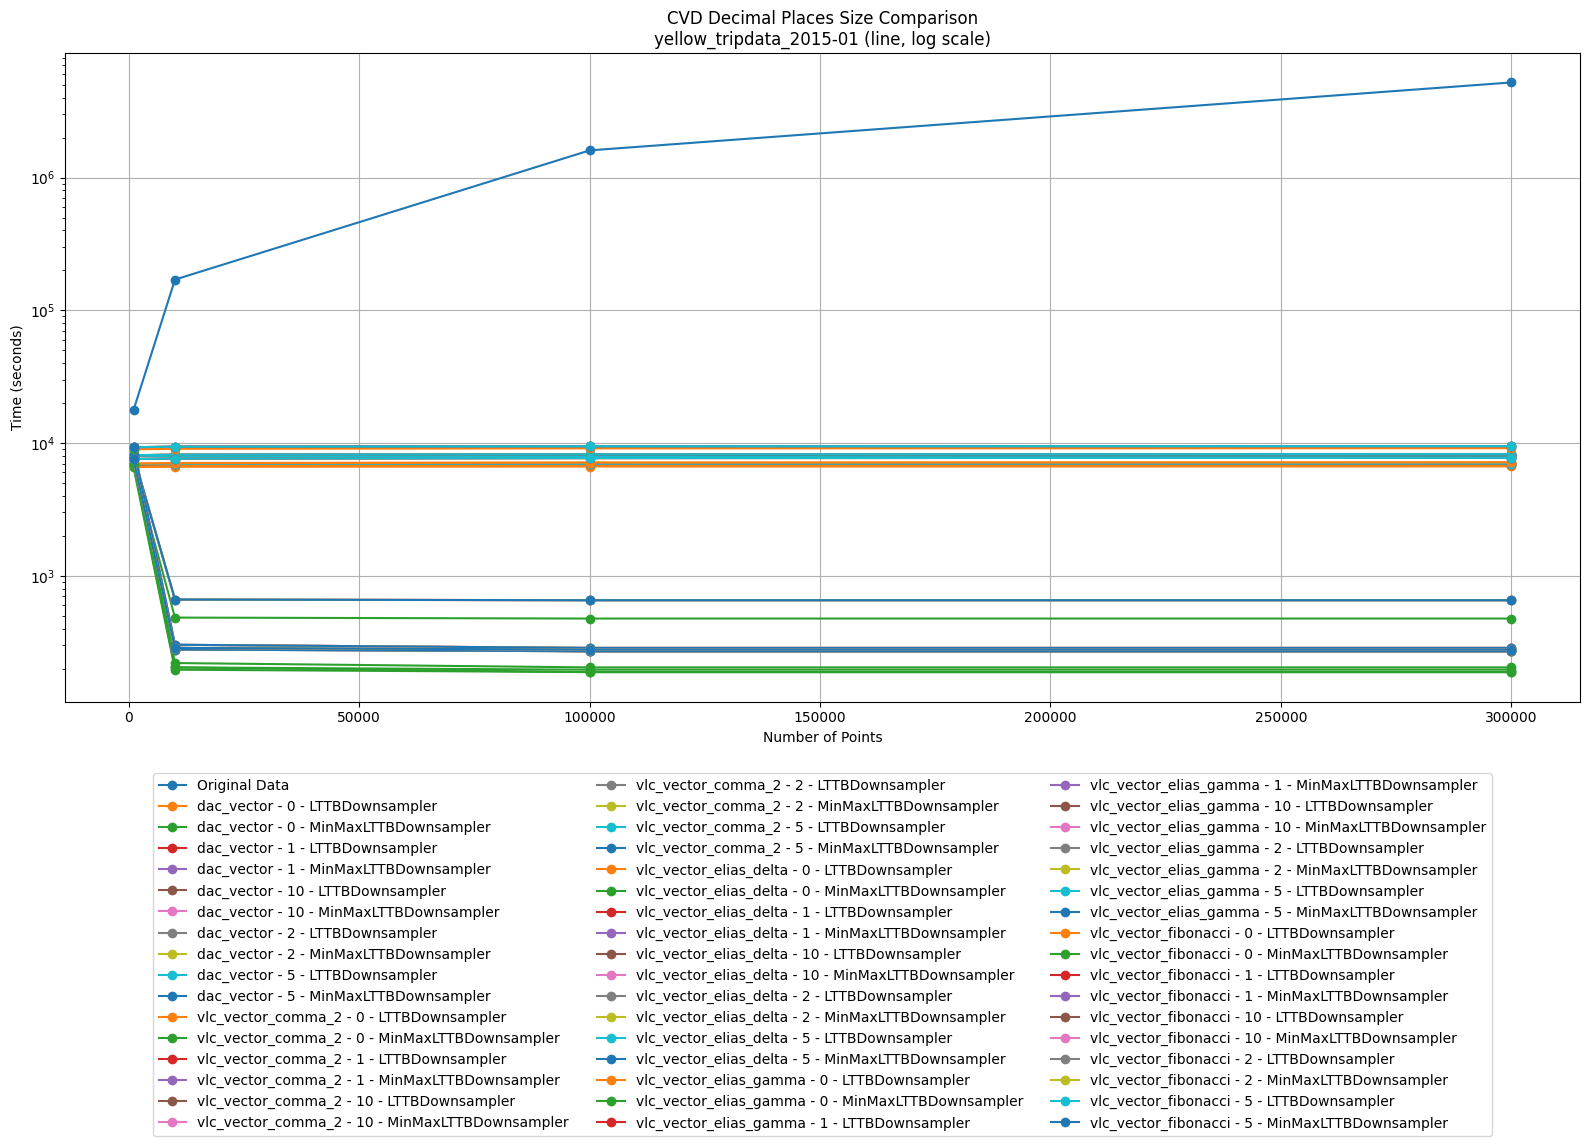
\includegraphics[width=1\textwidth]{anexo/exp/CVD Decimal Places Size Comparison/plots/CVD Decimal Places Size Comparison_yellow_tripdata_2015-01_log_line.png}
        \caption[]{Gráfico de tamaño CVD con diferentes lugares decimales para el input \textbf{yellow\_tripdata\_2015\_01} en escala logarítmica.}
        \label{fig:cvd_decimal_places_size_comparison_plot_log_3}
    \end{figure}
}





% PyGal Memory Allocation
\DeclareRobustCommand{\PyGalMemoryAllocationOnePlotLine}{
    %insertar imagen
    \begin{figure}[H]
        \centering
        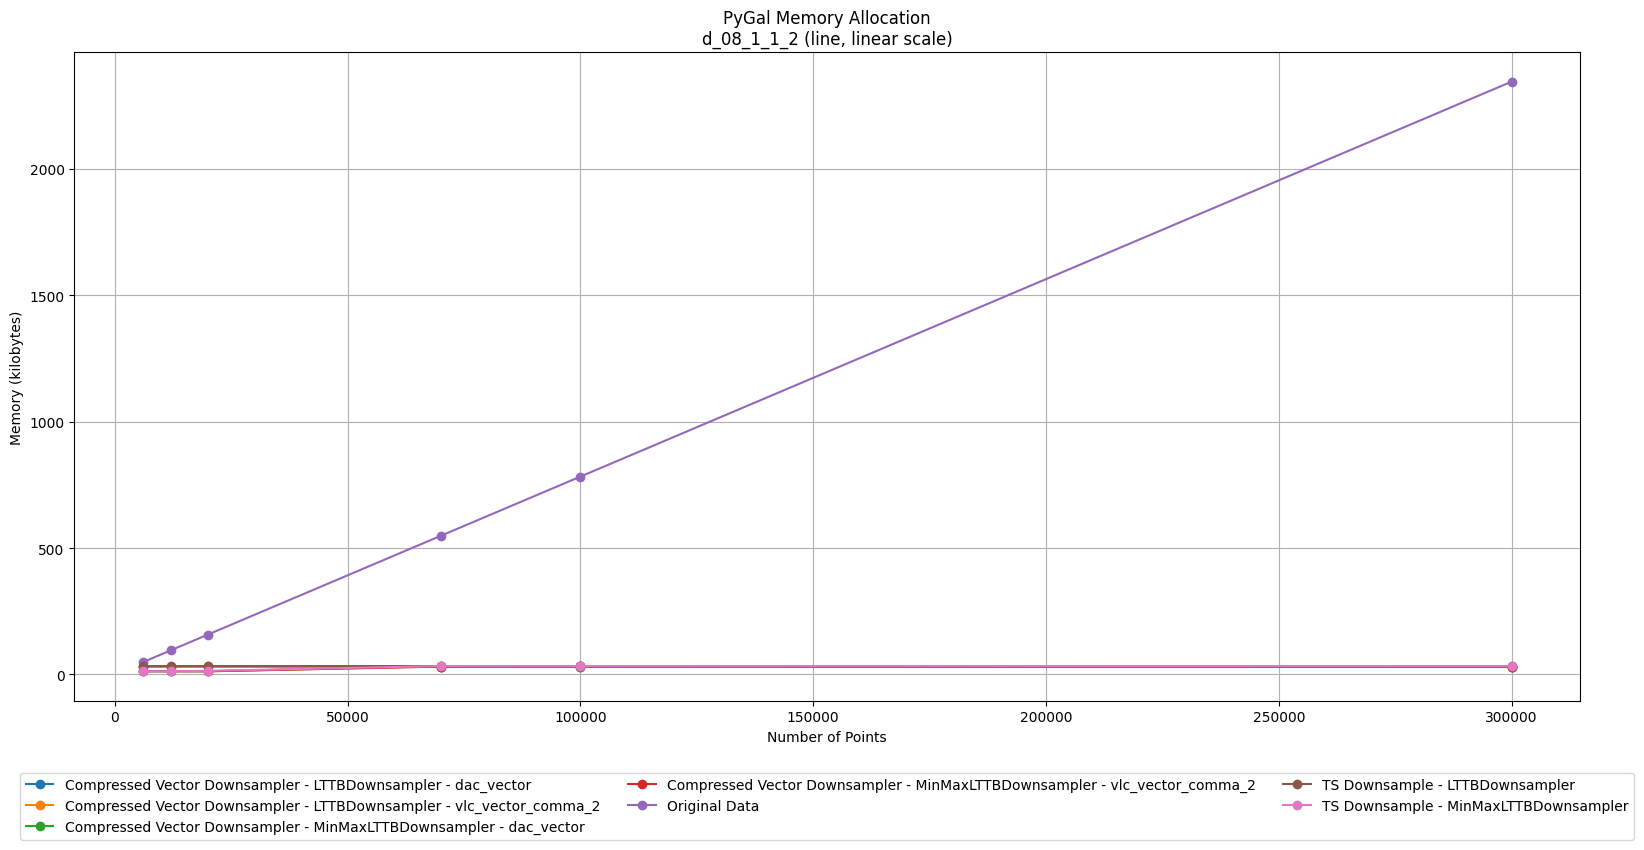
\includegraphics[width=1\textwidth]{anexo/exp/PyGal Memory Allocation/plots/PyGal Memory Allocation_d_08_1_1_2_linear_line.png}
        \caption[]{Gráfico de memoria asignada por PyGal para el input \textbf{d\_08\_1\_1\_2}.}
        \label{fig:pygal_memory_allocation_plot_line_1}
    \end{figure}
}

\DeclareRobustCommand{\PyGalMemoryAllocationOnePlotBar}{
    %insertar imagen
    \begin{figure}[H]
        \centering
        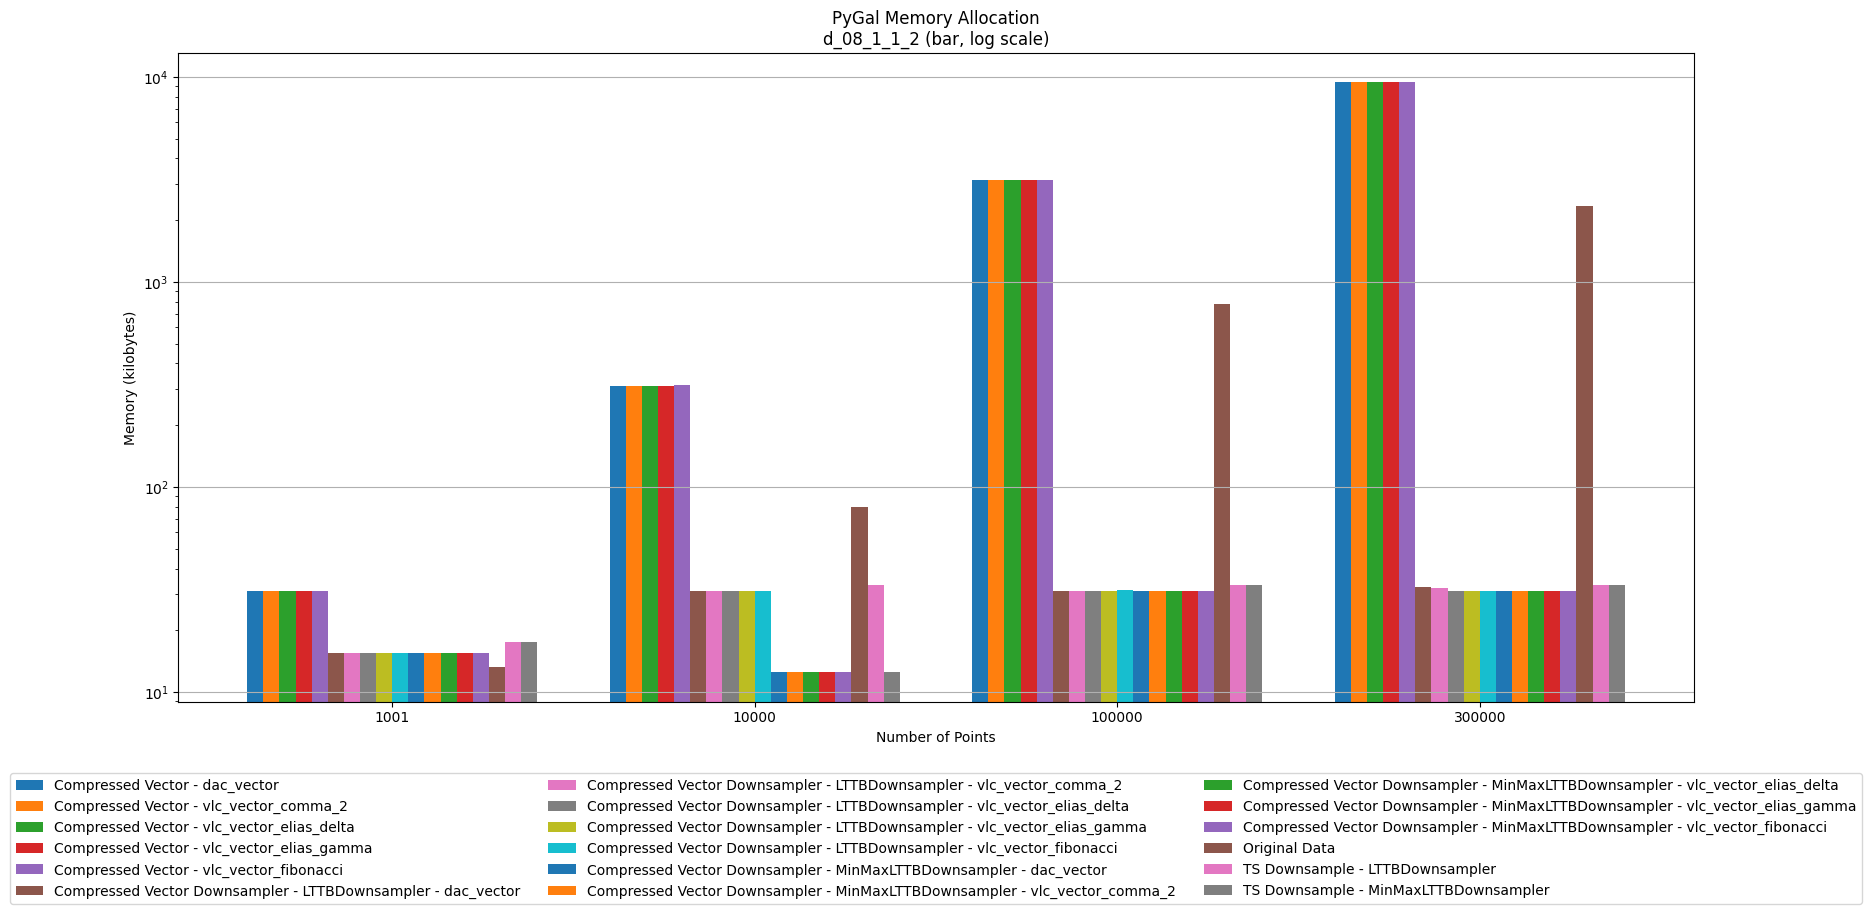
\includegraphics[width=1\textwidth]{anexo/exp/PyGal Memory Allocation/bar_plots/PyGal Memory Allocation_d_08_1_1_2_log_bar.png}
        \caption[]{Gráfico de memoria asignada por PyGal para el input \textbf{d\_08\_1\_1\_2}.}
        \label{fig:pygal_memory_allocation_plot_bar_1}
    \end{figure}
}

\DeclareRobustCommand{\PyGalMemoryAllocationTwoPlotLine}{
    %insertar imagen
    \begin{figure}[H]
        \centering
        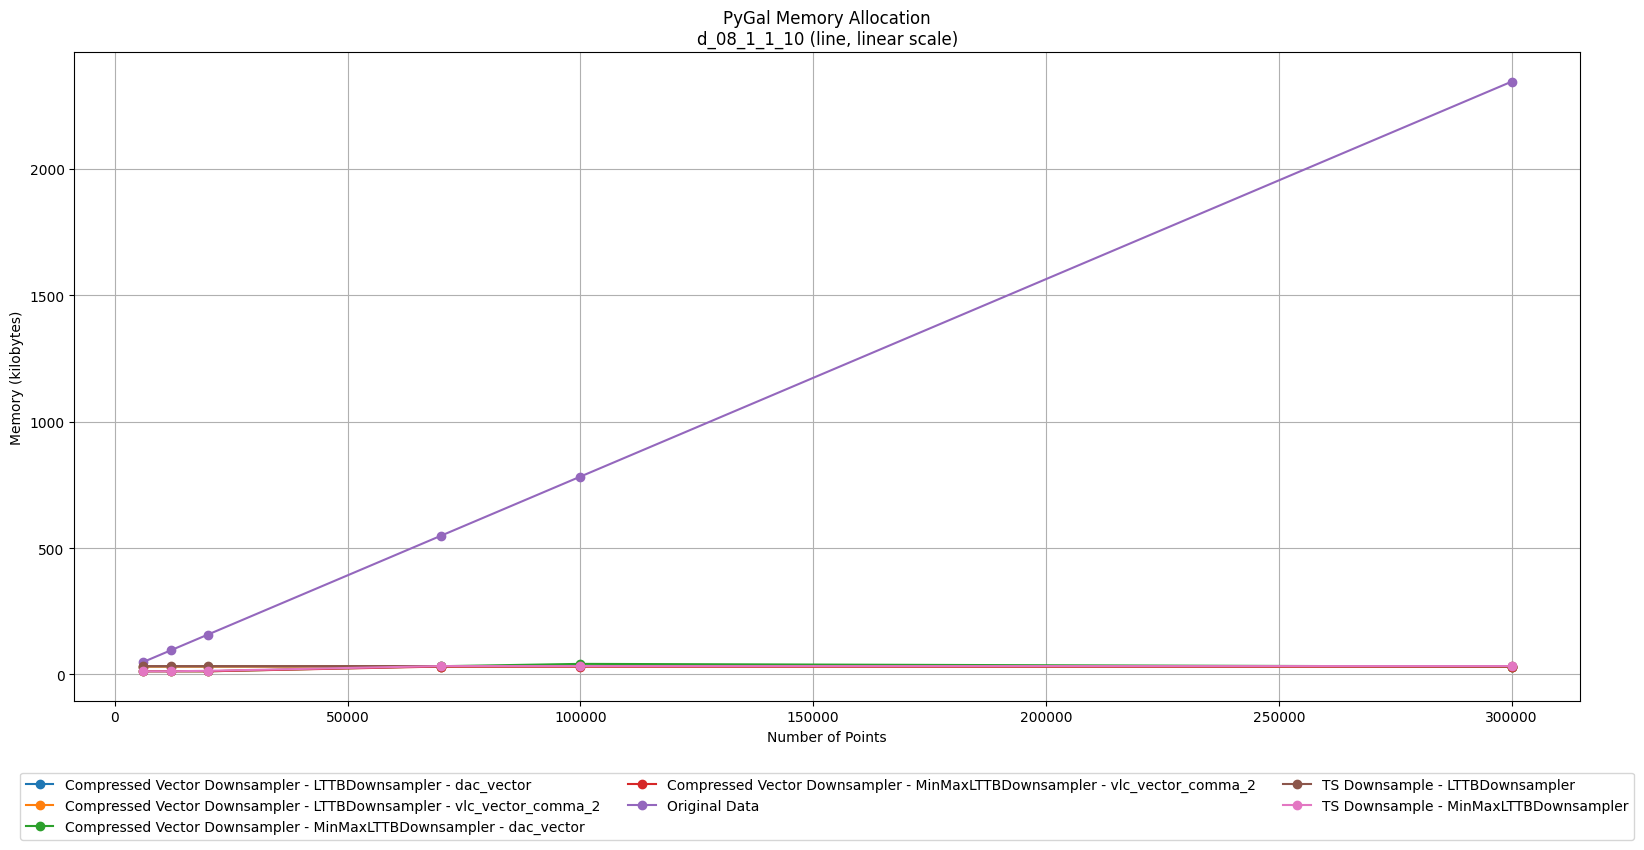
\includegraphics[width=1\textwidth]{anexo/exp/PyGal Memory Allocation/plots/PyGal Memory Allocation_d_08_1_1_10_linear_line.png}
        \caption[]{Gráfico de memoria asignada por PyGal para el input \textbf{d\_08\_1\_1\_10}.}
        \label{fig:pygal_memory_allocation_plot_line_2}
    \end{figure}
}

\DeclareRobustCommand{\PyGalMemoryAllocationTwoPlotBar}{
    %insertar imagen
    \begin{figure}[H]
        \centering
        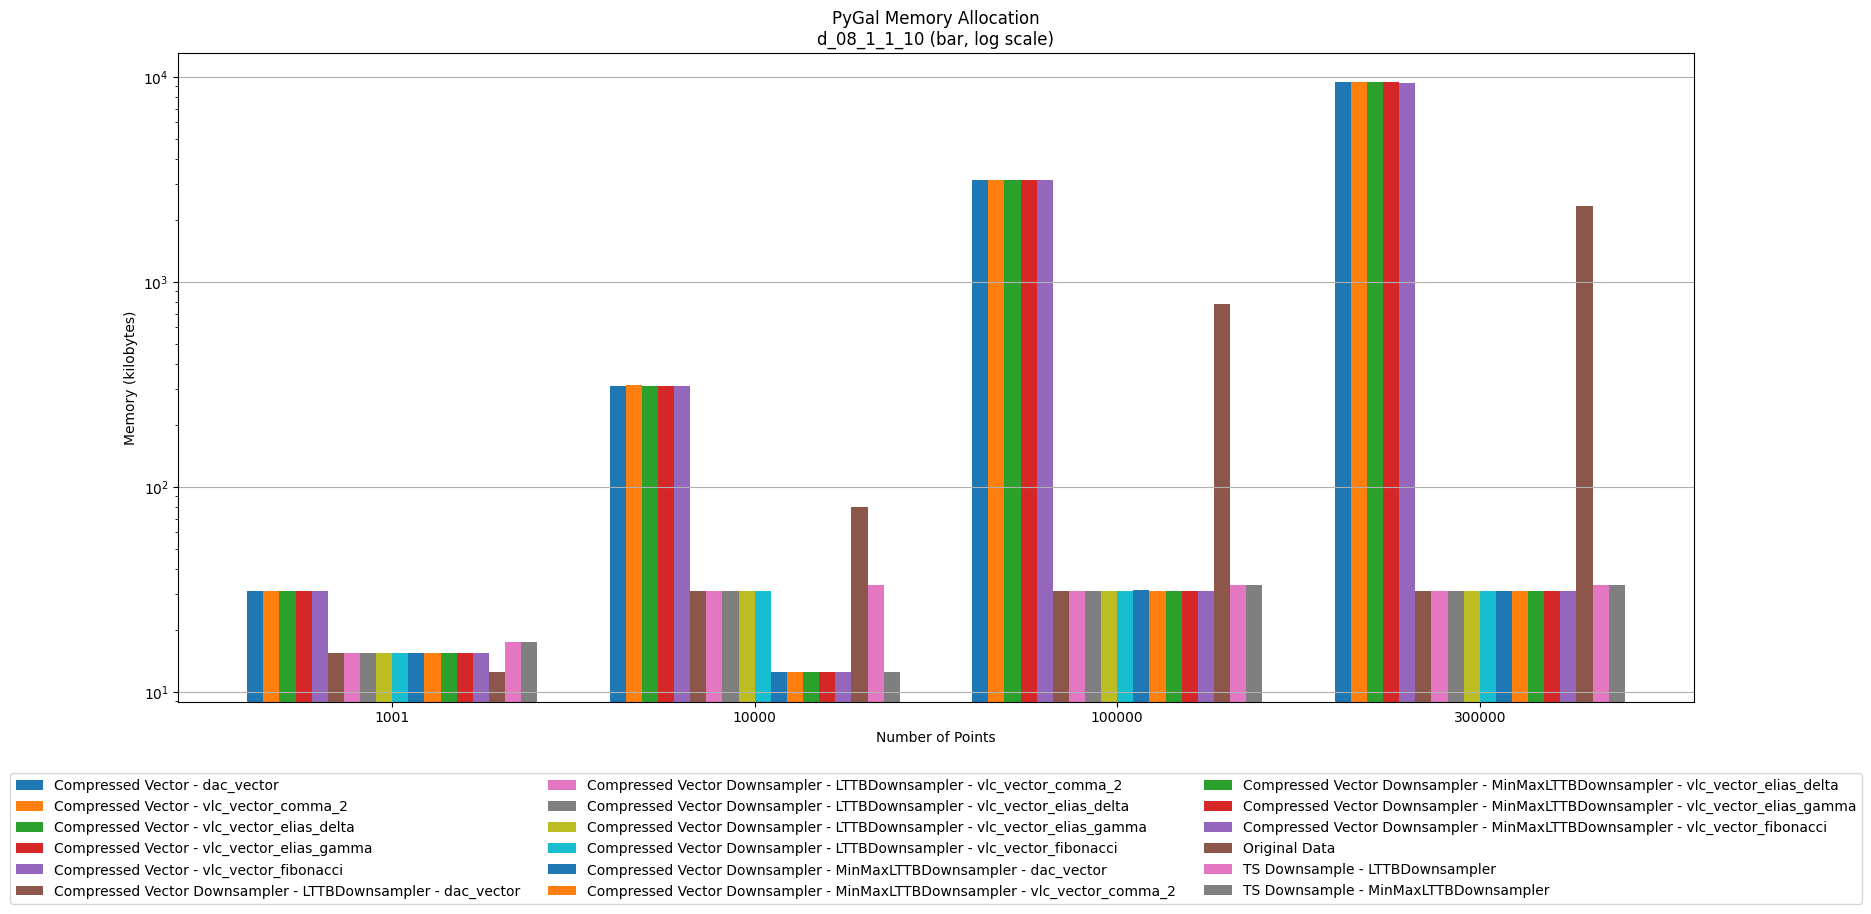
\includegraphics[width=1\textwidth]{anexo/exp/PyGal Memory Allocation/bar_plots/PyGal Memory Allocation_d_08_1_1_10_log_bar.png}
        \caption[]{Gráfico de memoria asignada por PyGal para el input \textbf{d\_08\_1\_1\_10}.}
        \label{fig:pygal_memory_allocation_plot_bar_2}
    \end{figure}
}

\DeclareRobustCommand{\PyGalMemoryAllocationThreePlotLine}{
    %insertar imagen
    \begin{figure}[H]
        \centering
        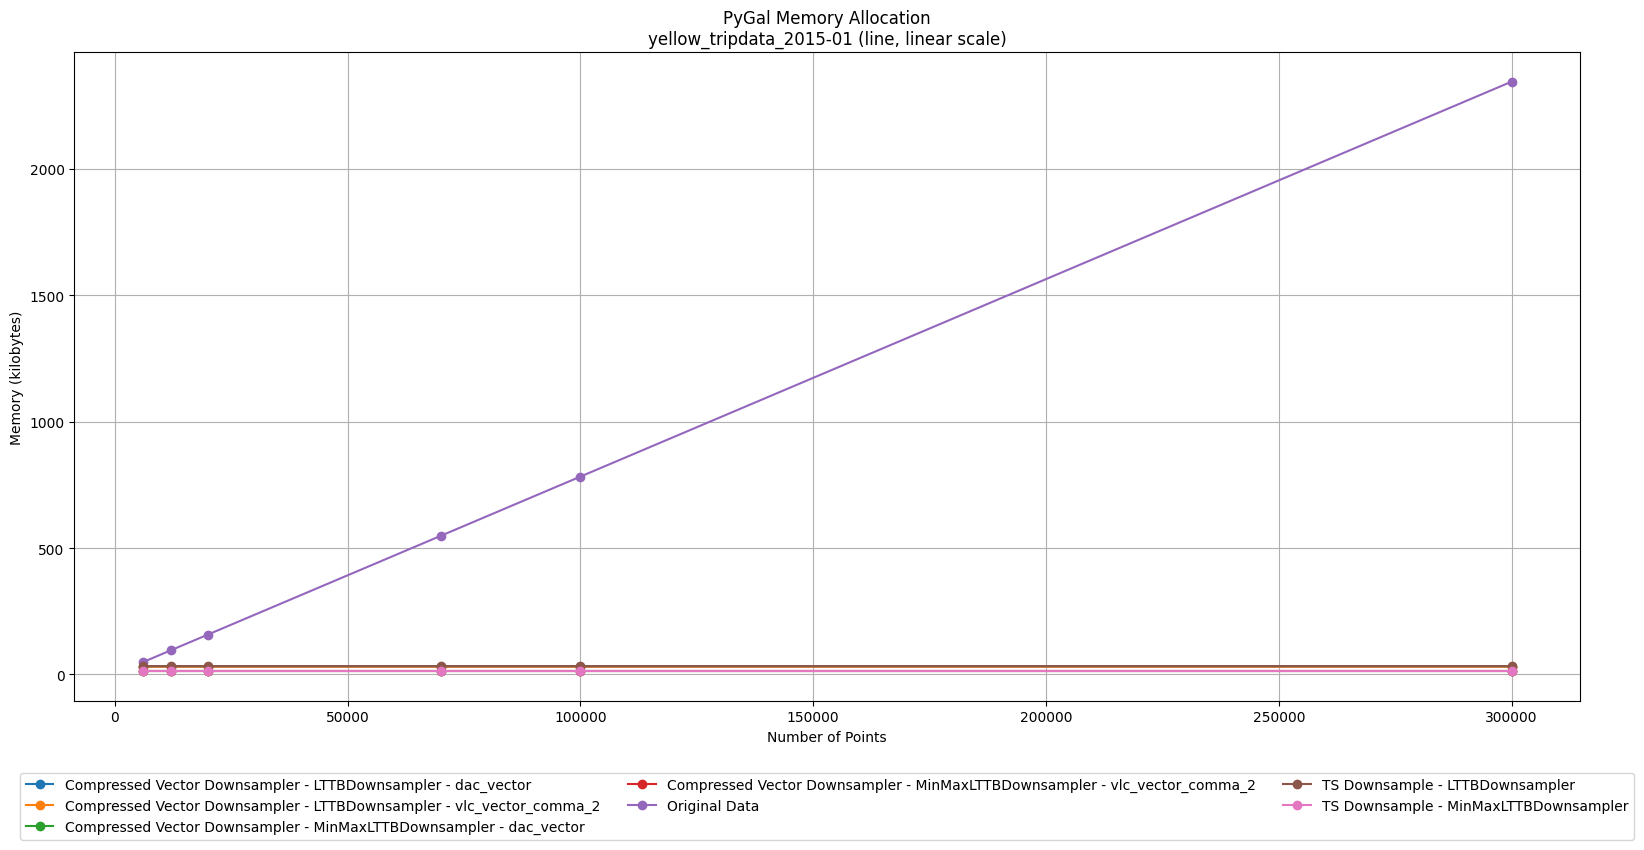
\includegraphics[width=1\textwidth]{anexo/exp/PyGal Memory Allocation/plots/PyGal Memory Allocation_yellow_tripdata_2015-01_linear_line.png}
        \caption[]{Gráfico de memoria asignada por PyGal para el input \textbf{yellow\_tripdata\_2015\_01}.}
        \label{fig:pygal_memory_allocation_plot_line_3}
    \end{figure}
}

\DeclareRobustCommand{\PyGalMemoryAllocationThreePlotBar}{
    %insertar imagen
    \begin{figure}[H]
        \centering
        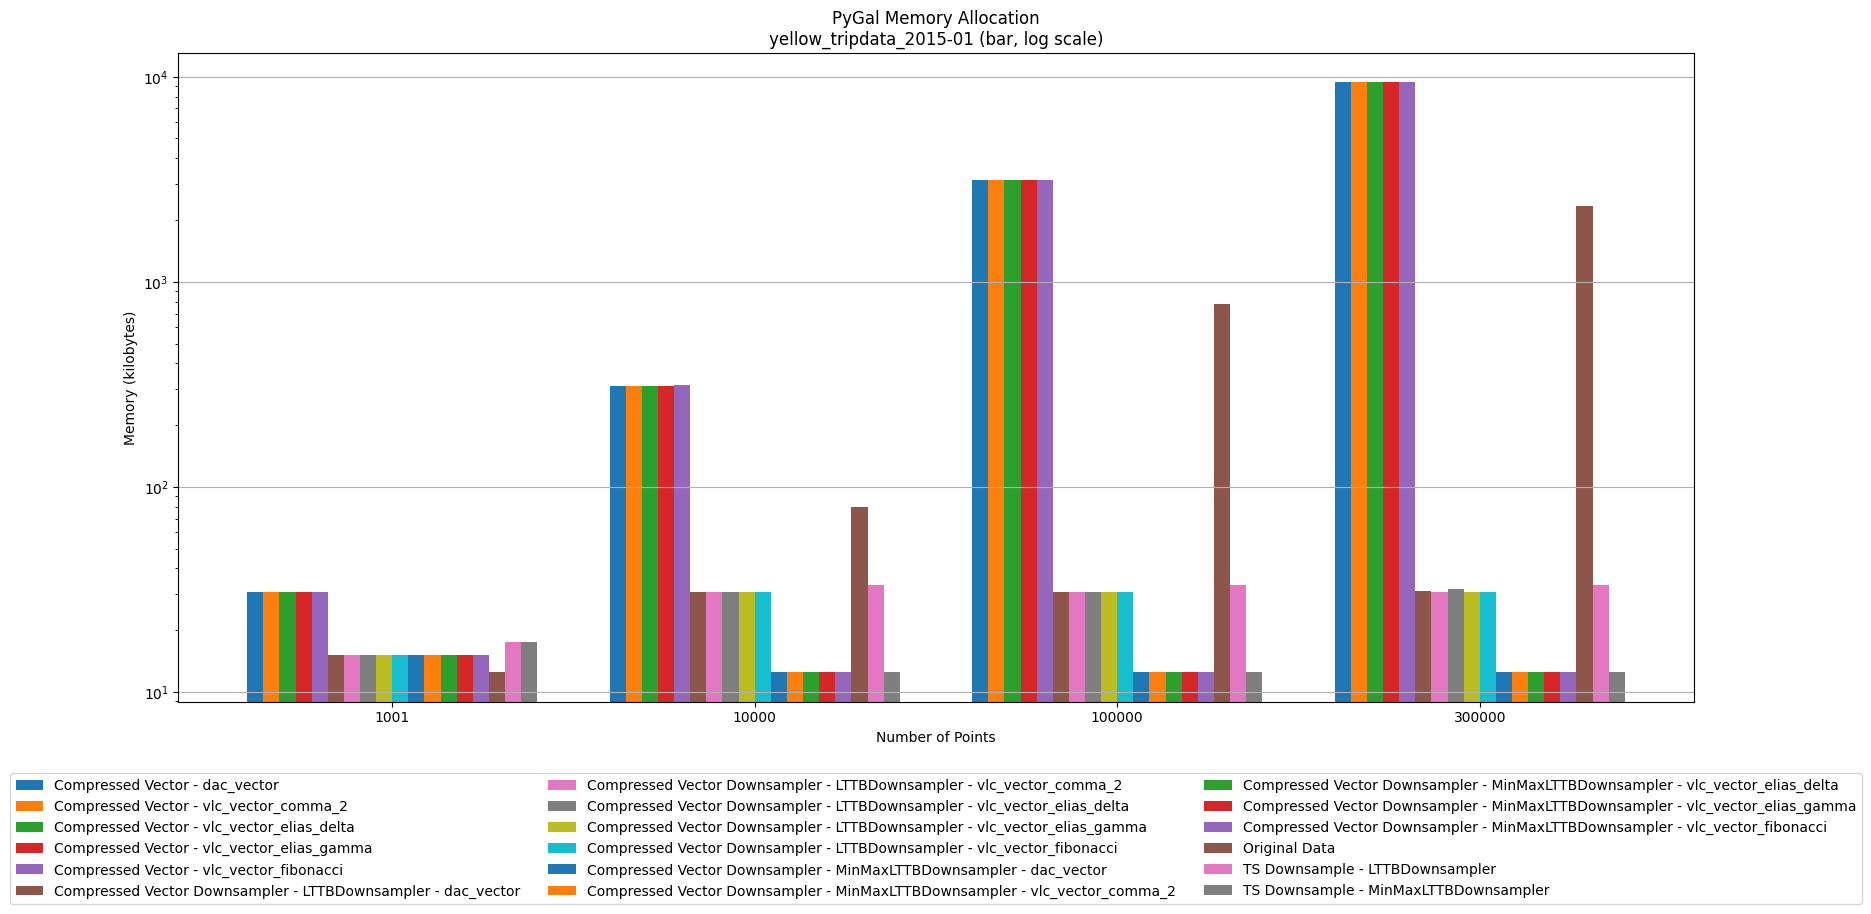
\includegraphics[width=1\textwidth]{anexo/exp/PyGal Memory Allocation/bar_plots/PyGal Memory Allocation_yellow_tripdata_2015-01_log_bar.png}
        \caption[]{Gráfico de memoria asignada por PyGal para el input \textbf{yellow\_tripdata\_2015\_01}.}
        \label{fig:pygal_memory_allocation_plot_bar_3}
    \end{figure}
}

% PyGal Plot Time
\DeclareRobustCommand{\PyGalPlotTimeOnePlotLine}{
    %insertar imagen
    \begin{figure}[H]
        \centering
        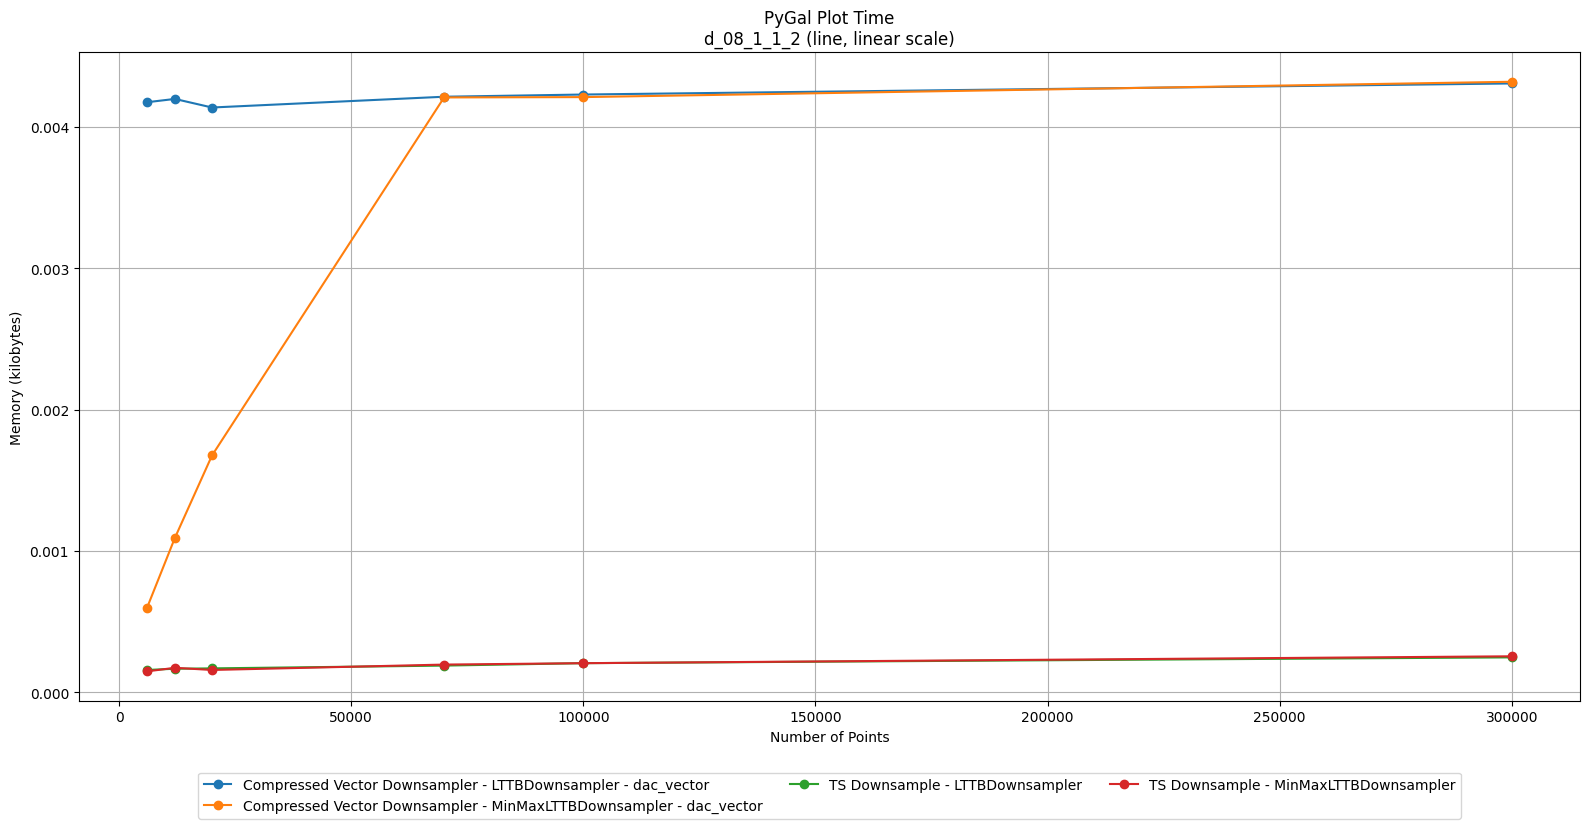
\includegraphics[width=1\textwidth]{anexo/exp/PyGal Plot Time/plots/PyGal Plot Time_d_08_1_1_2_linear_line.png}
        \caption[]{Gráfico de tiempo de renderización PyGal para el input \textbf{d\_08\_1\_1\_2}.}
        \label{fig:pygal_plot_time_plot_line_1}
    \end{figure}
    \begin{figure}[H]
        \centering
        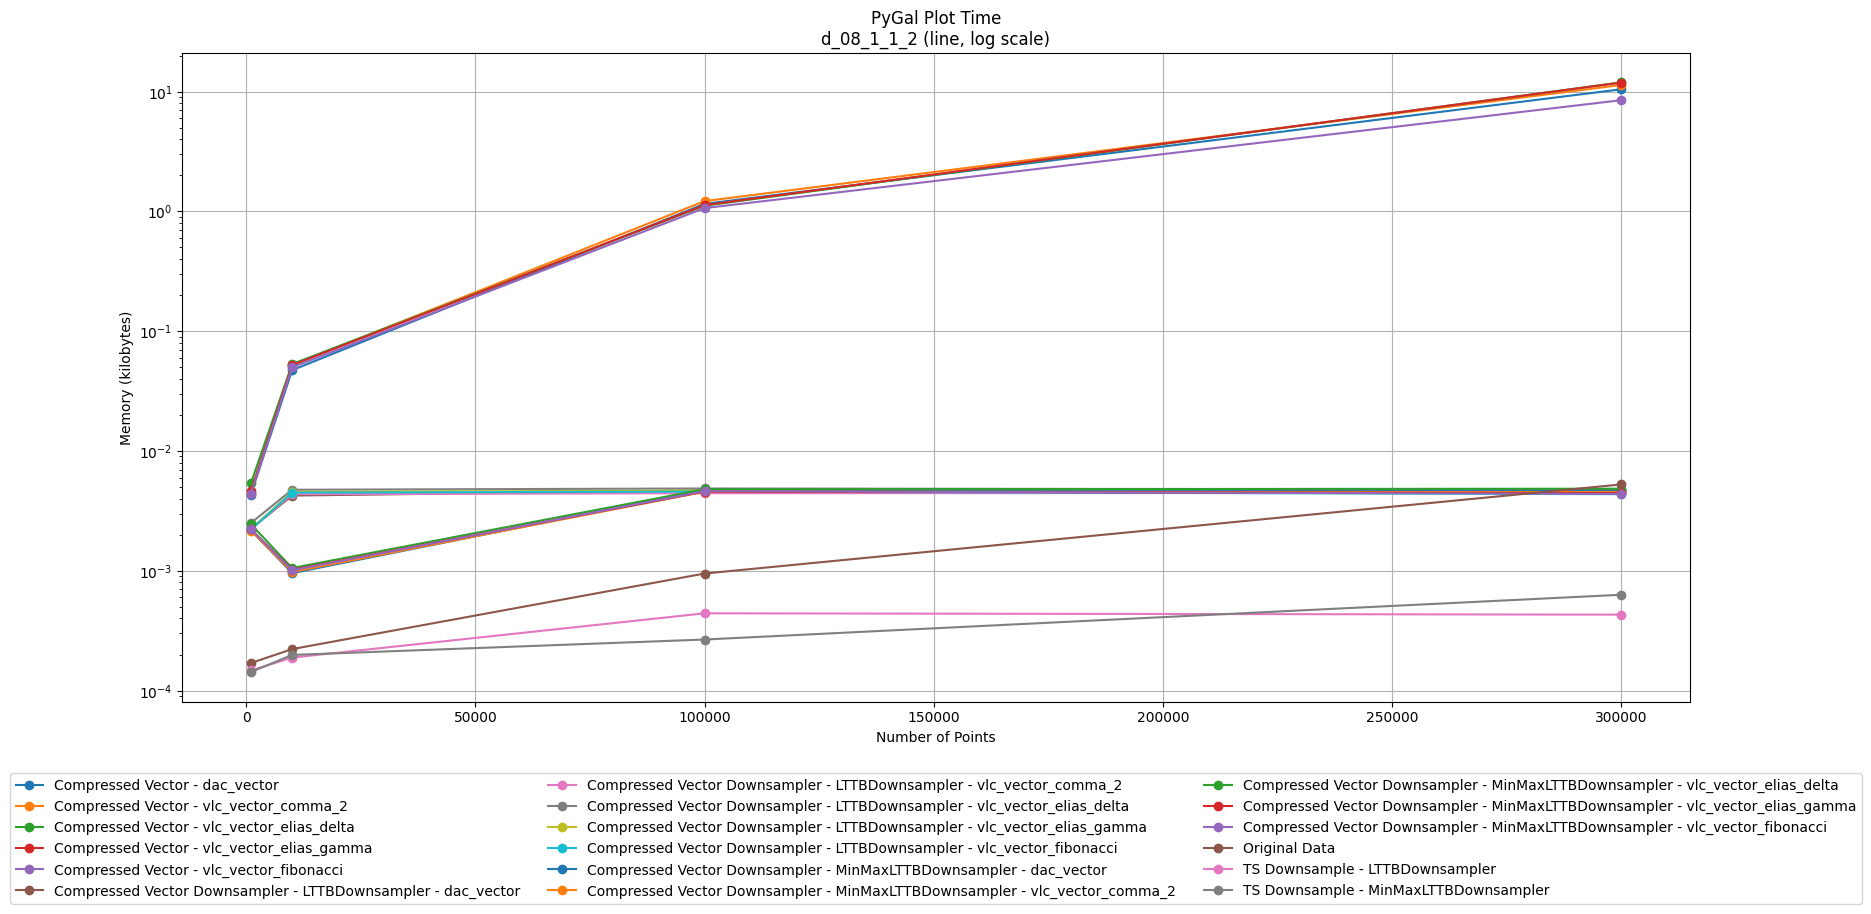
\includegraphics[width=1\textwidth]{anexo/exp/PyGal Plot Time/plots/PyGal Plot Time_d_08_1_1_2_log_line.png}
        \caption[]{Gráfico de tiempo de renderización PyGal para el input \textbf{d\_08\_1\_1\_2} en escala logarítmica.}
        \label{fig:pygal_plot_time_plot_line_1_log}
    \end{figure}
}

\DeclareRobustCommand{\PyGalPlotTimeOnePlotBar}{
    %insertar imagen
    \begin{figure}[H]
        \centering
        \includegraphics[width=1\textwidth]{anexo/exp/PyGal Plot Time/bar_plots/PyGal Plot Time_d_08_1_1_2_linear_bar.png}
        \caption[]{Gráfico de tiempo de renderización PyGal para el input \textbf{d\_08\_1\_1\_2}.}
        \label{fig:pygal_plot_time_plot_bar_1}
    \end{figure}
}

\DeclareRobustCommand{\PyGalPlotTimeTwoPlotLine}{
    %insertar imagen
    \begin{figure}[H]
        \centering
        \includegraphics[width=1\textwidth]{anexo/exp/PyGal Plot Time/plots/PyGal Plot Time_d_08_1_1_10_linear_line.png}
        \caption[]{Gráfico de tiempo de renderización PyGal para el input \textbf{d\_08\_1\_1\_10}.}
        \label{fig:pygal_plot_time_plot_line_2}
    \end{figure}
    \begin{figure}[H]
        \centering
        \includegraphics[width=1\textwidth]{anexo/exp/PyGal Plot Time/plots/PyGal Plot Time_d_08_1_1_10_log_line.png}
        \caption[]{Gráfico de tiempo de renderización PyGal para el input \textbf{d\_08\_1\_1\_10} en escala logarítmica.}
        \label{fig:pygal_plot_time_plot_line_2_log}
    \end{figure}
}

\DeclareRobustCommand{\PyGalPlotTimeTwoPlotBar}{
    %insertar imagen
    \begin{figure}[H]
        \centering
        \includegraphics[width=1\textwidth]{anexo/exp/PyGal Plot Time/bar_plots/PyGal Plot Time_d_08_1_1_10_linear_bar.png}
        \caption[]{Gráfico de tiempo de renderización PyGal para el input \textbf{d\_08\_1\_1\_10}.}
        \label{fig:pygal_plot_time_plot_bar_2}
    \end{figure}
}

\DeclareRobustCommand{\PyGalPlotTimeThreePlotLine}{
    %insertar imagen
    \begin{figure}[H]
        \centering
        \includegraphics[width=1\textwidth]{anexo/exp/PyGal Plot Time/plots/PyGal Plot Time_yellow_tripdata_2015-01_linear_line.png}
        \caption[]{Gráfico de tiempo de renderización PyGal para el input \textbf{yellow\_tripdata\_2015\_01}.}
        \label{fig:pygal_plot_time_plot_line_3}
    \end{figure}
    \begin{figure}[H]
        \centering
        \includegraphics[width=1\textwidth]{anexo/exp/PyGal Plot Time/plots/PyGal Plot Time_yellow_tripdata_2015-01_log_line.png}
        \caption[]{Gráfico de tiempo de renderización PyGal para el input \textbf{yellow\_tripdata\_2015\_01}.}
        \label{fig:pygal_plot_time_plot_line_3_log}
    \end{figure}
}

\DeclareRobustCommand{\PyGalPlotTimeThreePlotBar}{
    %insertar imagen
    \begin{figure}[H]
        \centering
        \includegraphics[width=1\textwidth]{anexo/exp/PyGal Plot Time/bar_plots/PyGal Plot Time_yellow_tripdata_2015-01_linear_bar.png}
        \caption[]{Gráfico de tiempo de renderización PyGal para el input \textbf{yellow\_tripdata\_2015\_01}.}
        \label{fig:pygal_plot_time_plot_bar_3}
    \end{figure}
}

\DeclareRobustCommand{\SDSLFourPyAccessTimeComparisonOnePlotBar}{
    \begin{figure}[H]
        \centering
        \includegraphics[width=1\textwidth]{anexo/exp/SDSL4Py Access Time Comparison/bar_plots/SDSL4Py Access Time Comparison_d_08_1_1_2_log_bar.png}
        \caption[]{Gráfico de tiempo de acceso SDSL4Py en escala logarítmica para el input \textbf{d\_08\_1\_1\_2}.}
        \label{fig:sdsl4py_access_time_comparison_plot_log_bar_1}
    \end{figure}
}

\DeclareRobustCommand{\SDSLFourPyAccessTimeComparisonTwoPlotBar}{
    \begin{figure}[H]
        \centering
        \includegraphics[width=1\textwidth]{anexo/exp/SDSL4Py Access Time Comparison/bar_plots/SDSL4Py Access Time Comparison_d_08_1_1_10_log_bar.png}
        \caption[]{Gráfico de tiempo de acceso SDSL4Py en escala logarítmica para el input \textbf{d\_08\_1\_1\_10}.}
        \label{fig:sdsl4py_access_time_comparison_plot_log_bar_2}
    \end{figure}
}

\DeclareRobustCommand{\SDSLFourPyAccessTimeComparisonThreePlotBar}{
    \begin{figure}[H]
        \centering
        \includegraphics[width=1\textwidth]{anexo/exp/SDSL4Py Access Time Comparison/bar_plots/SDSL4Py Access Time Comparison_yellow_tripdata_2015-01_log_bar.png}
        \caption[]{Gráfico de tiempo de acceso SDSL4Py en escala logarítmica para el input \textbf{yellow\_tripdata\_2015\_01}.}
        \label{fig:sdsl4py_access_time_comparison_plot_log_bar_3}
    \end{figure}
}

\DeclareRobustCommand{\SDSLFourPyCompressionSpaceComparisonOnePlotBar}{
    \begin{figure}[H]
        \centering
        \includegraphics[width=1\textwidth]{anexo/exp/SDSL4Py Compression Space Comparison/bar_plots/SDSL4Py Compression Space Comparison_d_08_1_1_2_log_bar.png}
        \caption[]{Gráfico de espacio de compresión SDSL4Py en escala logarítmica para el input \textbf{d\_08\_1\_1\_2}.}
        \label{fig:sdsl4py_compression_space_comparison_plot_log_bar_1}
    \end{figure}
}

\DeclareRobustCommand{\SDSLFourPyCompressionSpaceComparisonTwoPlotBar}{
    \begin{figure}[H]
        \centering
        \includegraphics[width=1\textwidth]{anexo/exp/SDSL4Py Compression Space Comparison/bar_plots/SDSL4Py Compression Space Comparison_d_08_1_1_10_log_bar.png}
        \caption[]{Gráfico de espacio de compresión SDSL4Py en escala logarítmica para el input \textbf{d\_08\_1\_1\_10}.}
        \label{fig:sdsl4py_compression_space_comparison_plot_log_bar_2}
    \end{figure}
}

\DeclareRobustCommand{\SDSLFourPyCompressionSpaceComparisonThreePlotBar}{
    \begin{figure}[H]
        \centering
        \includegraphics[width=1\textwidth]{anexo/exp/SDSL4Py Compression Space Comparison/bar_plots/SDSL4Py Compression Space Comparison_yellow_tripdata_2015-01_log_bar.png}
        \caption[]{Gráfico de espacio de compresión SDSL4Py en escala logarítmica para el input \textbf{yellow\_tripdata\_2015\_01}.}
        \label{fig:sdsl4py_compression_space_comparison_plot_log_bar_3}
    \end{figure}
}
\DeclareRobustCommand{\SDSLFourPyCompressionTimeComparisonOnePlotBar}{
    \begin{figure}[H]
        \centering
        \includegraphics[width=1\textwidth]{anexo/exp/SDSL4Py Compression Time Comparison/bar_plots/SDSL4Py Compression Time Comparison_d_08_1_1_2_log_bar.png}
        \caption[]{Gráfico de tiempo de compresión SDSL4Py en escala logarítmica para el input \textbf{d\_08\_1\_1\_2}.}
        \label{fig:sdsl4py_compression_time_comparison_plot_log_bar_1}
    \end{figure}
}

\DeclareRobustCommand{\SDSLFourPyCompressionTimeComparisonTwoPlotBar}{
    \begin{figure}[H]
        \centering
        \includegraphics[width=1\textwidth]{anexo/exp/SDSL4Py Compression Time Comparison/bar_plots/SDSL4Py Compression Time Comparison_d_08_1_1_10_log_bar.png}
        \caption[]{Gráfico de tiempo de compresión SDSL4Py en escala logarítmica para el input \textbf{d\_08\_1\_1\_10}.}
        \label{fig:sdsl4py_compression_time_comparison_plot_log_bar_2}
    \end{figure}
}

\DeclareRobustCommand{\SDSLFourPyCompressionTimeComparisonThreePlotBar}{
    \begin{figure}[H]
        \centering
        \includegraphics[width=1\textwidth]{anexo/exp/SDSL4Py Compression Time Comparison/bar_plots/SDSL4Py Compression Time Comparison_yellow_tripdata_2015-01_log_bar.png}
        \caption[]{Gráfico de tiempo de compresión SDSL4Py en escala logarítmica para el input \textbf{yellow\_tripdata\_2015\_01}.}
        \label{fig:sdsl4py_compression_time_comparison_plot_log_bar_3}
    \end{figure}
}


% Vega-Altair Plot Time Comparison
\DeclareRobustCommand{\VegaAltairPlotTimeComparisonOnePlotLine}{
    %insertar imagen
    \begin{figure}[H]
        \centering
        \includegraphics[width=1\textwidth]{anexo/exp/Vega-Altair Plot Time Comparison/plots/Vega-Altair Plot Time Comparison_d_08_1_1_2_linear_line.png}
        \caption[]{Gráfico de tiempo de renderización Vega-Altair para el input \textbf{d\_08\_1\_1\_2}.}
        \label{fig:vega_altair_plot_time_comparison_plot_line_1}
    \end{figure}
    \begin{figure}[H]
        \centering
        \includegraphics[width=1\textwidth]{anexo/exp/Vega-Altair Plot Time Comparison/plots/Vega-Altair Plot Time Comparison_d_08_1_1_2_log_line.png}
        \caption[]{Gráfico de tiempo de renderización Vega-Altair para el input \textbf{d\_08\_1\_1\_2} en escala logarítmica.}
        \label{fig:vega_altair_plot_time_comparison_plot_line_1}
    \end{figure}
}

\DeclareRobustCommand{\VegaAltairPlotTimeComparisonOnePlotBar}{
    %insertar imagen
    \begin{figure}[H]
        \centering
        \includegraphics[width=1\textwidth]{anexo/exp/Vega-Altair Plot Time Comparison/bar_plots/Vega-Altair Plot Time Comparison_d_08_1_1_2_linear_bar.png}
        \caption[]{Gráfico de tiempo de renderización Vega-Altair para el input \textbf{d\_08\_1\_1\_2}.}
        \label{fig:vega_altair_plot_time_comparison_plot_bar_1}
    \end{figure}
}

\DeclareRobustCommand{\VegaAltairPlotTimeComparisonTwoPlotLine}{
    %insertar imagen
    \begin{figure}[H]
        \centering
        \includegraphics[width=1\textwidth]{anexo/exp/Vega-Altair Plot Time Comparison/plots/Vega-Altair Plot Time Comparison_d_08_1_1_10_linear_line.png}
        \caption[]{Gráfico de tiempo de renderización Vega-Altair para el input \textbf{d\_08\_1\_1\_10}.}
        \label{fig:vega_altair_plot_time_comparison_plot_line_2}
    \end{figure}
    \begin{figure}[H]
        \centering
        \includegraphics[width=1\textwidth]{anexo/exp/Vega-Altair Plot Time Comparison/plots/Vega-Altair Plot Time Comparison_d_08_1_1_10_log_line.png}
        \caption[]{Gráfico de tiempo de renderización Vega-Altair para el input \textbf{d\_08\_1\_1\_10} en escala logarítmica.}
        \label{fig:vega_altair_plot_time_comparison_plot_line_2_log}
    \end{figure}
}

\DeclareRobustCommand{\VegaAltairPlotTimeComparisonTwoPlotBar}{
    %insertar imagen
    \begin{figure}[H]
        \centering
        \includegraphics[width=1\textwidth]{anexo/exp/Vega-Altair Plot Time Comparison/bar_plots/Vega-Altair Plot Time Comparison_d_08_1_1_10_linear_bar.png}
        \caption[]{Gráfico de tiempo de renderización Vega-Altair para el input \textbf{d\_08\_1\_1\_10}.}
        \label{fig:vega_altair_plot_time_comparison_plot_bar_2}
    \end{figure}
}

\DeclareRobustCommand{\VegaAltairPlotTimeComparisonThreePlotLine}{
    %insertar imagen
    \begin{figure}[H]
        \centering
        \includegraphics[width=1\textwidth]{anexo/exp/Vega-Altair Plot Time Comparison/plots/Vega-Altair Plot Time Comparison_yellow_tripdata_2015-01_linear_line.png}
        \caption[]{Gráfico de tiempo de renderización Vega-Altair para el input \textbf{yellow\_tripdata\_2015\_01}.}
        \label{fig:vega_altair_plot_time_comparison_plot_line_3}
    \end{figure}
    \begin{figure}[H]
        \centering
        \includegraphics[width=1\textwidth]{anexo/exp/Vega-Altair Plot Time Comparison/plots/Vega-Altair Plot Time Comparison_yellow_tripdata_2015-01_log_line.png}
        \caption[]{Gráfico de tiempo de renderización Vega-Altair para el input \textbf{yellow\_tripdata\_2015\_01} en escala logarítmica.}
        \label{fig:vega_altair_plot_time_comparison_plot_line_3_log}
    \end{figure}
}

\DeclareRobustCommand{\VegaAltairPlotTimeComparisonThreePlotBar}{
    %insertar imagen
    \begin{figure}[H]
        \centering
        \includegraphics[width=1\textwidth]{anexo/exp/Vega-Altair Plot Time Comparison/bar_plots/Vega-Altair Plot Time Comparison_yellow_tripdata_2015-01_linear_bar.png}
        \caption[]{Gráfico de tiempo de renderización Vega-Altair para el input \textbf{yellow\_tripdata\_2015\_01}.}
        \label{fig:vega_altair_plot_time_comparison_plot_bar_3}
    \end{figure}
}

% Vega-Altair Plotting + Building Comparison
\DeclareRobustCommand{\VegaAltairPlottingBuildingComparisonOnePlotLine}{
    %insertar imagen
    \begin{figure}[H]
        \centering
        \includegraphics[width=1\textwidth]{anexo/exp/Vega-Altair Plotting + Building Comparison/plots/Vega-Altair Plotting + Building Comparison_d_08_1_1_2_linear_line.png}
        \caption[]{Gráfico de tiempo de renderización y construcción Vega-Altair para el input \textbf{d\_08\_1\_1\_2}.}
        \label{fig:vega_altair_plotting_building_comparison_plot_line_1}
    \end{figure}
    \begin{figure}[H]
        \centering
        \includegraphics[width=1\textwidth]{anexo/exp/Vega-Altair Plotting + Building Comparison/plots/Vega-Altair Plotting + Building Comparison_d_08_1_1_2_log_line.png}
        \caption[]{Gráfico de tiempo de renderización y construcción Vega-Altair para el input \textbf{d\_08\_1\_1\_2} en escala logarítmica.}
        \label{fig:vega_altair_plotting_building_comparison_plot_line_1}
    \end{figure}
}

\DeclareRobustCommand{\VegaAltairPlottingBuildingComparisonOnePlotBar}{
    %insertar imagen
    \begin{figure}[H]
        \centering
        \includegraphics[width=1\textwidth]{anexo/exp/Vega-Altair Plotting + Building Comparison/bar_plots/Vega-Altair Plotting + Building Comparison_d_08_1_1_2_linear_bar.png}
        \caption[]{Gráfico de tiempo de renderización y construcción Vega-Altair para el input \textbf{d\_08\_1\_1\_2}.}
        \label{fig:vega_altair_plotting_building_comparison_plot_bar_1}
    \end{figure}
}

\DeclareRobustCommand{\VegaAltairPlottingBuildingComparisonTwoPlotLine}{
    %insertar imagen
    \begin{figure}[H]
        \centering
        \includegraphics[width=1\textwidth]{anexo/exp/Vega-Altair Plotting + Building Comparison/plots/Vega-Altair Plotting + Building Comparison_d_08_1_1_10_linear_line.png}
        \caption[]{Gráfico de tiempo de renderización y construcción Vega-Altair para el input \textbf{d\_08\_1\_1\_10}.}
        \label{fig:vega_altair_plotting_building_comparison_plot_line_2}
    \end{figure}
    \begin{figure}[H]
        \centering
        \includegraphics[width=1\textwidth]{anexo/exp/Vega-Altair Plotting + Building Comparison/plots/Vega-Altair Plotting + Building Comparison_d_08_1_1_10_linear_line.png}
        \caption[]{Gráfico de tiempo de renderización y construcción Vega-Altair para el input \textbf{d\_08\_1\_1\_10} en escala logarítmica.}
        \label{fig:vega_altair_plotting_building_comparison_plot_line_2}
    \end{figure}
}

\DeclareRobustCommand{\VegaAltairPlottingBuildingComparisonTwoPlotBar}{
    %insertar imagen
    \begin{figure}[H]
        \centering
        \includegraphics[width=1\textwidth]{anexo/exp/Vega-Altair Plotting + Building Comparison/bar_plots/Vega-Altair Plotting + Building Comparison_d_08_1_1_10_linear_bar.png}
        \caption[]{Gráfico de tiempo de renderización y construcción Vega-Altair para el input \textbf{d\_08\_1\_1\_10}.}
        \label{fig:vega_altair_plotting_building_comparison_plot_bar_2}
    \end{figure}
}

\DeclareRobustCommand{\VegaAltairPlottingBuildingComparisonThreePlotLine}{
    %insertar imagen
    \begin{figure}[H]
        \centering
        \includegraphics[width=1\textwidth]{anexo/exp/Vega-Altair Plotting + Building Comparison/plots/Vega-Altair Plotting + Building Comparison_yellow_tripdata_2015-01_linear_line.png}
        \caption[]{Gráfico de tiempo de renderización y construcción Vega-Altair para el input \textbf{yellow\_tripdata\_2015\_01}.}
        \label{fig:vega_altair_plotting_building_comparison_plot_line_3}
    \end{figure}
    \begin{figure}[H]
        \centering
        \includegraphics[width=1\textwidth]{anexo/exp/Vega-Altair Plotting + Building Comparison/plots/Vega-Altair Plotting + Building Comparison_yellow_tripdata_2015-01_linear_line.png}
        \caption[]{Gráfico de tiempo de renderización y construcción Vega-Altair para el input \textbf{yellow\_tripdata\_2015\_01} en escala logarítmica.}
        \label{fig:vega_altair_plotting_building_comparison_plot_line_3}
    \end{figure}
}

\DeclareRobustCommand{\VegaAltairPlottingBuildingComparisonThreePlotBar}{
    %insertar imagen
    \begin{figure}[H]
        \centering
        \includegraphics[width=1\textwidth]{anexo/exp/Vega-Altair Plotting + Building Comparison/bar_plots/Vega-Altair Plotting + Building Comparison_yellow_tripdata_2015-01_linear_bar.png}
        \caption[]{Gráfico de tiempo de renderización y construcción Vega-Altair para el input \textbf{yellow\_tripdata\_2015\_01}.}
        \label{fig:vega_altair_plotting_building_comparison_plot_bar_3}
    \end{figure}
}
